\documentclass[12pt,oneside]{book}
\usepackage{graphicx}
\usepackage{subcaption}
\usepackage{color}
\usepackage{amscd,amsfonts,amssymb,amsmath,amsthm}
\usepackage[utf8]{inputenc}
\usepackage[T1]{fontenc}
\usepackage[english]{babel}
\usepackage[all]{xy}
\usepackage{enumerate}
\usepackage[a4paper]{geometry}
\usepackage{fancyhdr}
\usepackage{tabularx}
\usepackage{makeidx}
\usepackage[backend=biber,style=numeric,sorting=nyt]{biblatex}
\usepackage{hyperref}
\usepackage{xcolor}

\definecolor{navyblue}{rgb}{0.0, 0.0, 0.5}

\addbibresource{referencias.bib}

\geometry{textwidth=150mm,textheight=247mm,top=30mm,bottom=30mm,left=30mm,right=30mm,headsep=10mm,
footskip=10mm}


\pagestyle{fancy}
\fancyhead[LO]{\rightmark}
\fancyhead[RO]{\thepage}
\fancyfoot[C]{\empty}

\makeindex

\newtheorem{defi}   {Definition}[chapter]
\newtheorem{teo}    {Theorem}[chapter]
\newtheorem{ex}     {Example}[chapter]
\newtheorem{prop}   {Proposition}[chapter]
\newtheorem{lem}    {Lemma}[chapter]
\newtheorem{cor}    {Corollary}[chapter]
\newtheorem{obs}    {Observation}[chapter]
\newtheorem{conj}	{Conjecture}

\newcommand{\ds}{\displaystyle}
\newcommand{\R}{\mathbb{R}}
\newcommand{\RP}{\mathbb{R}P}
\newcommand{\Z}{\mathbb{Z}}
\newcommand{\F}{\mathbb{F}}
\newcommand{\ccup}{\smile}
\newcommand{\ccap}{\frown}
\newcommand{\tensor}{\otimes}
\newcommand{\wt}{\widetilde}





\begin{document}





    \fontfamily{ptm}\selectfont

    \begin{titlepage}
        \begin{center}
            \textbf{FEDERAL UNIVERSITY OF SÃO CARLOS}
        \end{center}

        \vspace{-0.8cm}

        \begin{center}  
            \fontsize{10}{12}\selectfont CENTER OF EXACT SCIENCES AND TECHNOLOGY
        \end{center}

        \vspace{-0.8cm}

        \begin{center}
            \fontsize{10}{12}\selectfont GRADUATE PROGRAM IN MATHEMATICS
        \end{center}

        \vspace{3cm}

        \begin{center}
            \small{Alex Melges Barbosa}
        \end{center}

        \vspace{3cm}

        \begin{center}
            \Large{\textbf{Characteristic Classes of \\ Topological and Generalized Manifolds}}
        \end{center}

        \vspace{10cm}

        \begin{center}
            São Carlos - SP/Brazil
        \end{center}

        \vspace{-0.8cm}

        \begin{center}
            2022
        \end{center}
    \end{titlepage}



    \newpage
    \thispagestyle{empty}

    \begin{center}
        \small{Alex Melges Barbosa}

        \scriptsize{\href{mailto:exemplo@dominio.com}{\textcolor{navyblue}{melges.ab@gmail.com}}}

        \scriptsize{\href{https://www.linkedin.com/in/alexmelgesbarbosa/}{ \textcolor{navyblue}{LinkedIn profile}}}

        \scriptsize{\href{https://github.com/alex-melges}{\textcolor{navyblue}{GitHub profile}}}
    \end{center}

    \vspace{3cm}

    \begin{center}
        \Large{\textbf{Characteristic Classes of \\ Topological and Generalized Manifolds}}
    \end{center}

    \vspace{2cm}

    \begin{flushright}
        \begin{minipage}{0.55\textwidth}
            Thesis submitted to the Graduate Program in Mathematics at the Federal University of 
            São Carlos as part of the requirements for the degree of PhD in Mathematics \\[0.5cm] 
            Advisor: Prof. Dr. Edivaldo Lopes dos Santos

            \hspace{1.7cm}\scriptsize{\href{mailto:exemplo@dominio.com}{\textcolor{navyblue}{edivaldo@ufscar.br}}}
        \end{minipage}
    \end{flushright}

    \vfill

    \begin{center}
        São Carlos - SP/Brazil
    \end{center}

    \vspace{-0.8cm}

    \begin{center}
        03/24/2022
    \end{center}



    \newpage
    \thispagestyle{empty}

    \vspace{\fill}

    \begin{flushright}
        \begin{minipage}{5cm}
            \begin{flushright}
                \vspace{22cm}\textit{To my parents \\ Antonio Carlos and Edith \\ and my siblings \\ 
                Carol and André.}
            \end{flushright}
        \end{minipage}
    \end{flushright}



    \newpage
    \chapter*{Acknowledgements}
    \thispagestyle{empty}
    \

    First of all, I would like to thank God for the opportunities and doors that have opened throughout 
    my 11-year academic journey, spanning my undergraduate, master’s, and doctoral degrees. There have 
    been many moments—both good and challenging—that have shaped me into the person and professional I 
    am today.

    I would also like to express my gratitude to my parents, Antonio Carlos and Edith, and my siblings, 
    Carol and André, who have been my unwavering support every day.

    A special thanks goes to two individuals who have been my mentors throughout this process: Edivaldo 
    and João Peres. They have not only helped shape me into the mathematician I am today but, more 
    importantly, have played a key role in shaping the person I’ve become. Thank you both very much.

    Last but not least, I want to thank my friends, who have been like a second family to me during this 
    long journey. There’s no need for me to mention them by name, as only those who have lifted me up 
    during my stumbles and celebrated my successes with me truly understand the depth of my gratitude 
    and affection for them.

    This work was supported financially by CAPES.



    \vspace{2cm}

    \begin{center}
        \begin{minipage}{10cm}
            \textit{In memory of my father, Antonio Carlos Barbosa. Unfortunately, you couldn't be 
            physically present on the day of my defense, but you certainly were and will always be 
            present in the hearts of our entire family. Thank you for everything!}
        \end{minipage}
    \end{center}



    \newpage
    \thispagestyle{empty}

    \begin{flushright}
        \begin{minipage}{8cm}
            \begin{flushright}
                \vspace{22cm}\textit{Either you have a strategy,\\
                or you're part of someone else's strategy.}

                \vspace{0.2cm} Alvin Toffler
            \end{flushright}
        \end{minipage}
    \end{flushright}



    \chapter*{Abstract}
    \thispagestyle{empty}

    In this work, we will first present generalized bundles, a concept developed by Fadell with the aim 
    of generalizing vector bundles, Stiefel-Whitney classes, and Wu's formula from the context of smooth 
    manifolds to topological manifolds. After that, we will use generalized bundles to obtain original 
    results concerning the Thom, Stiefel-Whitney, Wu, and Euler classes of topological manifolds, as 
    well as to provide a second proof of Wu's formula for topological manifolds and to establish the 
    topological version of the Poincaré-Hopf Theorem. Finally, we will use Poincaré and 
    Poincaré-Lefschetz dualities to construct the Stiefel-Whitney classes of generalized manifolds in a 
    broader manner, aiming to present, for the first time in the literature, a proof of Wu's formula 
    for such manifolds.

    \

    \noindent Keywords: characteristic classes, generalized bundles, topological manifolds, generalized 
    manifolds, Wu's formula.



    \tableofcontents
    \thispagestyle{empty}

    \listoffigures
    \thispagestyle{empty}



    \chapter*{List of Notations}
    \thispagestyle{empty}

    \begin{enumerate}
        \item Saying that $f:X\to Y$ is a map means the same as saying that $f$ is a continuous function 
        between topological spaces.
        \item $f:X \rightleftarrows Y:g$ denotes two maps when $f:X\to Y$ and $g:Y\to X$, not necessarily 
        inverses of each other. 
        \item $1:X\to X$ denotes the identity map on $X$.
        \item $f^{-1}$ denotes the preimage of a map $f$, as well as its inverse mapping (when it exists).
        \item If $f:X\to Y$ is a map, then $f(\_)$ denotes $f(x)$ for every $x\in X$.
        \item If $H:X\times Y\to Z$ is a map defined on a Cartesian product, then $H(\_,y)$ denotes 
        $H(x,y)$ for every $x\in X$. The same holds for $H(x,\_)$.
        \item $p_{i}:X_{1}\times \cdots\times X_{n}\to X_{i}$ denotes the projection on the $i$-th factor.
        \item $d:X\to X\times X$ denotes the diagonal map\index{diagonal!map} given by $d(x)=(x,x)$.
        \item Saying that $U\subset X$ is an open neighborhood of some subset $A\subset X$ means the 
        same as saying that $U$ is an open subspace of $X$ that contains $A$.
        \item Saying that $\mathcal{U}$ is an open cover of a topological space $B$ means the same as 
        saying that $\mathcal{U}=\{ U\subset B \}$, such that $U\subset B$ is an open subspace of $B$ 
        for every $U\in\mathcal{U}$ and $\ds\bigcup_{U\in\mathcal{U}}U=B$.  
        \item $X \approx Y$ denotes when two topological spaces are homeomorphic.
        \item $f \sim g$ denotes when two maps are homotopic.
        \item $X\sim Y$ denotes when two topological spaces have the same type of homotopy.
        \item $G_{1}\cong G_{2}$ denotes when two algebraic objects are, appropriately, isomorphic.
        \item $\mathbb{S}^{n-1}=\{ x\in\R^{n} \ : \ \| x \|=1 \}$.
        \item $D^{n}=\{ x\in\R^{n} \ : \ \| x \|\leq1 \}$.
        \item $B^{n}=\{ x\in\R^{n} \ : \ \| x \|<1 \}$.
        \item $I=[0,1]\subset \R$.
        \item $X^{I}$ denotes the topological space of paths in $X$.
        \item $\Omega(X,x_{0})=\{ \omega\in X^{I} \ : \ \omega(0)=\omega(1)=x_{0} \}$.
        \item $H_{k}(X,A;R)$ and $H^{k}(X,A;R)$ denote the $k$-th $R$-modules of singular homology and 
        cohomology, respectively, of the pair $(X,A)$ with coefficients in a commutative ring $R$ with 
        unity.
        \item $H_{k}^{c}(X,A;R)$ and $H^{k}_{c}(X,A;R)$ denote, respectively, the $k$-th $R$-modules of 
        singular homology and cohomology with compact support.
        \item $\wt{H}_{k}(X,A;R)$ and $\wt{H}^{k}(X,A;R)$ denote, respectively, the $k$-th $R$-modules of 
        reduced singular homology and cohomology.
        \item $\check{H}^{k}(X,A;R)$ denotes the $k$-th $R$-module of Čech cohomology.
        \item $H^{k}(X,A;R)=(x)$ denotes that the $k$-th $R$-module of cohomology of the pair $(X,A)$ is 
        generated by the element $x\in H^{k}(X,A;R)$. The same applies for homology modules.
        \item If $x\in H^{k}(X,A;R)$, then we denote $|x|=k$. The same applies for homology modules.
        \item $<,>:H^{k}(X,A;R)\tensor H_{k}(X,A;R)\to R$ denotes the Kronecker product, which maps 
        $\varphi\tensor\sigma\mapsto <\varphi,\sigma>$.
        \item $\ccap:H_{k}(X,A\cup B;R)\tensor H^{l}(X,A;R)\to H_{k-l}(X,B;R)$ denotes the cap product, 
        which maps $\sigma\tensor\varphi\mapsto\sigma\ccap\varphi$.
        \item $\ccup:H^{k}(X,A;R)\tensor H^{l}(X,B;R)\to H^{k+l}(X,A\cup B;R)$ denotes the cup product, 
        which maps $\varphi\tensor\psi\mapsto\varphi\ccup\psi$.
        \item $\times:H^{k}(X,A;R)\tensor H^{l}(Y,B;R)\to H^{k+l}(X\times Y,(X\times B)\cup(A\times Y);R)$ 
        denotes the cross product, which maps $\varphi\tensor\psi\mapsto\varphi\times\psi$.
        \thispagestyle{empty}
    \end{enumerate}





    \chapter{Introduction}
    \thispagestyle{empty}

    \

    \textit{"Between the 4th and 10th of September 1935, during the International Congress of Topology 
    held in Moscow, several works were presented that would forever change the future of Algebraic 
    Topology, with some of these works now considered foundational research lines in this theory. 
    Among these works, we can mention:
        \begin{itemize}
            \item The introduction by Witold Hurewicz to homotopy groups.
            \item The lectures by Heinz Hopf and Hassler Whitney on vector fields and sphere bundles, 
            which initiated the study of vector bundles and, consequently, characteristic classes.
            \item The independent introductions by James Alexander and Andrei Kolmogorov to cohomology 
            theory, as well as the cup product."
        \end{itemize}}
    
    \
    
    In this work, we will contribute to the theory of characteristic classes, more specifically, 
    characteristic classes of topological and generalized manifolds.
    
    After this historical context on the emergence of characteristic class theory, we will begin 
    introducing the basic concepts used for the development of this work.
    
    In 1955, Nash introduced in \cite{nash} the concept that would become known as the field of 
    non-singular paths of a topological manifold, which can be understood as the topological version of 
    a non-zero vector field. Essentially, Nash showed that given a smooth manifold $M$ and fixing a 
    point $b\in M$, the space of non-zero tangent vectors of $M$ at $b$ can also be defined from the 
    topological viewpoint, up to a homotopy equivalence, as the set:
    $$\{ \omega \in M^{I} : \omega(t) = b \Leftrightarrow t = 0 \}$$

    \
    
    A decade later, in 1965, Fadell defined in \cite{fadell_1} generalized bundles, a concept that 
    not only generalized vector bundles, but also allowed the extension, through Nash's ideas in 
    \cite{nash}, of the notions of tangent and normal fiber bundles from the context of smooth manifolds 
    to topological manifolds. Furthermore, Fadell constructed the Stiefel-Whitney classes of generalized 
    fiber bundles in order to obtain Whitney's duality for specific topological embeddings and to prove 
    the Wu formula for topological manifolds.
    
    The theory developed by Fadell in \cite{fadell_1} will serve as the foundation for the development 
    of our entire work, which can be divided into two parts:
        \begin{itemize}
            \item The first part will consist of chapters \ref{cap_fib}, \ref{cap_clas_carac}, and 
            \ref{cap_aplic}. These chapters can be interpreted as a modern re-reading of the results 
            obtained by Fadell in \cite{fadell_1}, as well as a continuation of the same, since we will 
            present additional results both on generalized bundles themselves and on Thom, 
            Stiefel-Whitney, Euler, and Wu classes of topological manifolds.
            \item The second part of this work will consist solely of chapter \ref{cap_wu_gen}, in which 
            we will construct more extensively the Stiefel-Whitney classes of generalized manifolds in 
            order to present for the first time in the literature a proof of the Wu formula for such 
            manifolds.
        \end{itemize}
    
        \
    
    Now, we will look in more detail at how we will organize the structure of our work, pointing out our 
    contributions and the relevance of the results that will be presented here.

    \
    
    In chapter \ref{cap_fib}, we will begin our work by presenting the studies conducted on generalized 
    fiber bundles\index{generalized!fiber bundle}, a tool developed by Fadell in \cite{fadell_1}, which 
    not only generalized the concepts of tangent and normal vector bundles from the context of smooth 
    manifolds to topological manifolds, but also allowed him to define the 
    Stiefel-Whitney\index{Stiefel-Whitney!class} classes and prove Whitney's 
    duality\index{Whitney!duality} and the Wu formula\index{Wu!formula} for the context of topological 
    manifolds\index{topological!manifold}.
    
    Concatenating definitions \ref{PLH}, \ref{defi_par-fib}, and \ref{defi_fib_gen}, we can define a 
    generalized bundle more directly as follows:

    \

        \textbf{Definition. } \textit{Given $E$ and $B$ topological spaces, $E_{0}\subset E$ and 
        $p:E\to B$ a onto map, we call the pair $(\mathcal{F},\mathcal{F}_{0})=(E,E_{0},p,B)$ an 
        $\R^{n}-$generalized bundle when:
            \hspace{1cm}\begin{enumerate}
                \item For any maps $h:X\to E$ and $H:X\times I\to B$, such that $H(\_,0)=p\circ h$, 
                there exists a map $\wt{H}:X\times I\to E$ such that $\wt{H}(\_,0)=h$ and 
                $p\circ\wt{H}=H$.
                \item If $x_{0}\in X$ is such that $h(x_{0})\in E_{0}$, then $\wt{H}(x_{0},\_)\in E_{0}$.
                \item There exists a map $s:B\to E$ such that $E_{0}=E-s(B)$.
                \item For all $b\in B$, $(p^{-1}(b),p^{-1}(b)\bigcap E_{0})\sim (\R^{n},\R^{n}-\{0\})$.
            \end{enumerate}}
    
    \

    With this definition, we can interpret a generalized bundle as a fibration with the following 
    characteristics:
        \begin{itemize}
            \item The total space is a pair of topological spaces.
            \item There is always at least one global section.
            \item The fiber behaves, up to homotopy equivalence, like a Euclidean space.
        \end{itemize}
    
    \
    
    During the reading of Chapter \ref{cap_fib}, the reader will notice that the development of the 
    chapter will not be as straightforward compared to the definition above, since our main goal 
    will be to present the theory of generalized bundles in a more detailed way and using a more 
    modern language than the results presented by Fadell in the first half of \cite{fadell_1}.

    More explicitly, we will show in Example \ref{fht_fv} how generalized bundles indeed generalize 
    vector bundles, and in Proposition \ref{iso_fv_fht} how the notion of isomorphism between vector 
    bundles remains valid when extended to the category of generalized bundles. We will also show that 
    it is possible to construct new generalized bundles from others, just as it happens with vector 
    bundles, for example: restriction bundles, product bundles, and Whitney sum bundles.

    Although Chapter \ref{cap_fib} is a preliminary chapter, we will contribute with original results 
    concerning the pullback generalized bundle, which was developed by Brown in \cite{brown} but was 
    neither cited nor used by Fadell in \cite{fadell_1}. These results will prove to be quite relevant 
    when we use them in the construction of some maps regarding characteristic classes of topological 
    manifolds in Chapters \ref{cap_clas_carac} and \ref{cap_aplic}.

    \

    In Chapter \ref{cap_clas_carac}, we will address the topic of characteristic classes of generalized 
    bundles and topological manifolds, more specifically, Thom classes, Stiefel-Whitney classes, and 
    Euler classes. Initially, we will introduce the notion of $R-$orientability of generalized bundles, 
    where $R$ is a commutative ring with unity, and their respective Thom classes, concepts originally 
    proposed by Fadell in \cite{fadell_1}, but little explored by him, since the main topic developed 
    in the second half of \cite{fadell_1} was about Stiefel-Whitney classes, in which case orientability 
    is not a concern.

    Thus, we will detail a little more the definition of $R-$orientability of generalized bundles and 
    present some technical results on the behavior of Thom classes under pullback and product generalized 
    bundles, as well as show what happens when we reverse the orientability of a generalized bundle and 
    the relation between the dimension of a $\Z-$orientable topological manifold and the Thom class of 
    its tangent generalized bundle. Even though these results are already known in the context of vector 
    bundles and smooth manifolds, they can be considered original since they have not yet been described 
    in the context of generalized bundles and topological manifolds.

    The second topic we will address in Chapter \ref{cap_clas_carac} will be about Stiefel-Whitney 
    classes. The purpose of this topic will be to rewrite the main properties and consequences of these 
    classes, already widespread in the literature, for the context of generalized bundles and topological 
    manifolds, following the same steps used by Milnor in (\cite{milnor_1}, Chapter 8) for vector bundles 
    and smooth manifolds. In doing so, we will offer a broader, more modern, and detailed reinterpretation 
    of the results proposed by Fadell in the second half of \cite{fadell_1}. Our contributions to this 
    topic will involve results concerning pullback generalized bundles.

    The third and last topic addressed in Chapter \ref{cap_clas_carac} will be about Euler classes. 
    Differently from Stiefel-Whitney classes, Euler classes can only be defined for $\Z-$orientable 
    generalized bundles. Thus, due to the technical lemmas related to Thom classes of $\Z-$orientable 
    generalized bundles obtained at the beginning of Chapter \ref{cap_clas_carac}, we will be able to 
    conclude several consequences and applications concerning Euler classes of generalized bundles and 
    $\Z-$orientable topological manifolds. In this topic, except for Proposition \ref{euler_2}, all other 
    results will be original, being generalizations of known results about Euler classes for vector 
    bundles and smooth manifolds. Among these generalizations, we highlight:

    \

        \textbf{Proposition 3.7.} \textit{Let $(\mathcal{F},\mathcal{F}_{0})=(E,E_{0},p,B)$ be an 
        $\R^{n}-$generalized bundle that is $\Z$-orientable. If $(\mathcal{F},\mathcal{F}_{0})$ admits a 
        section $s:B\to E$ such that $s(B)\subset E_{0}$, then 
        $e(\mathcal{F},\mathcal{F}_{0})=0$.}\footnote{$e(\mathcal{F},\mathcal{F}_{0})$ will denote the Euler 
        class of the generalized bundle $(\mathcal{F},\mathcal{F}_{0})$.}
    
    \

    The proposition above, in its version for vector bundles, is widely known, as it allows interpreting 
    the Euler class of a vector bundle as an obstruction to the existence of a nowhere-vanishing section. 
    In this work, we will present the generalized version of this interpretation, which will allow us to 
    obtain the main application related to the Euler class in Chapter \ref{cap_aplic}, the topological 
    version of the Poincaré-Hopf theorem.

    Up to this point, the reader should already have noticed the main goal of Chapters \ref{cap_fib} and 
    \ref{cap_clas_carac} of our work, which is to structure in detail and using a more up-to-date 
    language the theory of generalized bundles and their characteristic classes, while also presenting 
    several technical contributions, aiming to generalize applications regarding characteristic classes 
    of smooth manifolds to the context of topological manifolds, as we will see next.

    \

    The conclusion of our work regarding characteristic classes of generalized bundles will be presented 
    in Chapter \ref{cap_aplic}, where we will present three major applications with original technical 
    proofs concerning Stiefel-Whitney, Euler, and Wu classes of closed topological manifolds. Initially, 
    we will present an alternative proof of the topological version of the famous Wu formula, which 
    relates the Stiefel-Whitney and Wu classes of a smooth manifold through Steenrod squares.

    In \cite{fadell_1}, Fadell uses generalized bundles to give a first proof of Wu's formula for 
    topological manifolds, based on the techniques used by Milnor in (\cite{milnor_2}, Chapter 9). 
    Furthermore, the preliminary results that Fadell develops to prove Wu's formula are all in the 
    framework of singular (co)homology $\Z_{2}-$modules. Meanwhile, the alternative proof of Wu's 
    formula for topological manifolds that we will present in Chapter \ref{cap_aplic} will be based on 
    different techniques also introduced by Milnor, now found in (\cite{milnor_1}, Chapter 11).

    Comparing the proofs presented by us in this work and by Fadell in \cite{fadell_1}, the main 
    differences will be found in the preliminary lemmas used in Wu's formula, as we will prove them in 
    the framework of singular (co)homology $R-$modules with $R=\Z$ or $R=\Z_{2}$. Since we will use the 
    same sequence of results employed by Milnor in \cite{milnor_1}, now using generalized bundles 
    instead of vector bundles, our main contribution will be obtaining the case $R=\Z$ of the following 
    result:

    \

        \textbf{Lemma 4.1.} \textit{Let $M^{m}$ be a closed, connected, $R$-orientable topological manifold 
        with $R=\Z$ or $R=\Z_{2}$, $b\in M$ arbitrary, 
        $j_{b}:(M,M-\{b\})\hookrightarrow (M\times M,(M\times M)-\Delta)$ the canonical inclusion, 
        $[M]_{b}\in H_{m}(M,M-\{b\};R)$ the local $R$-orientation class of $M$ at $b$, and 
        $(\tau')\in H^{m}(M\times M,(M\times M)-\Delta;R)$ the generator uniquely defined by the Thom class 
        of the tangent generalized bundle of $M$. Then:
            $$ <j_{b}^{*}(\tau'),[M]_{b}>=1\in R $$}
    
    \

    The proof of the lemma above, in its version for smooth manifolds, can be found in (\cite{milnor_1}, 
    Lemma 11.7, p. 123), where the Riemannian structure of the manifold and the existence of the 
    exponential map are used, whereas our proof will be entirely algebraic, allowing generalization to 
    the context of topological manifolds, which will be crucial for the topological applications of the 
    Euler class.

    The second application of Chapter \ref{cap_aplic} will concern Euler classes. In fact, we will 
    present two applications on this topic, one being the relation between the Euler class and the Euler 
    characteristic of a topological manifold, and the other being the topological version of the 
    Poincaré-Hopf theorem. The reader will notice the importance of the $R=\Z$ case of Lemma 4.1 for the 
    first application, whose statement is as follows:

    \

        \textbf{Theorem 4.2. }\textit{If $M$ is a closed, connected, and $\Z$-orientable topological 
        manifold, then\footnote{$e(M)$, $[M]$, and $\chi(M)$ will denote, respectively, the Euler class, 
        the global orientation class, and the Euler characteristic of the manifold $M$.}:
        $$ <e(M),[M]>=\chi(M> $$}

    \

    For the second map involving the Euler class, we will need to define the concept of a path field on 
    a topological manifold, which was introduced by Nash in \cite{nash} as follows:
    
    \

        \textbf{Definition 4.1. }\textit{A path field on a topological manifold $M$ is any section of its 
        generalized bundle $(\tau M,\tau_{0}M)=(TM,T_{0}M,p,M)$. Moreover, a nonsingular path field on $M$ 
        is a section $s:M\to TM$ such that $s(M)\subset T_{0}M$.}

    \

    As we will show in Chapter \ref{cap_aplic}, generalized bundles will allow us to generalize the 
    notion of nowhere-vanishing vector fields from the smooth manifold context to the topological 
    manifold setting, since a smooth manifold admits a nowhere-vanishing vector field if and only if it 
    admits a nonsingular path field. With that, we will be able to prove the topological version of the 
    Poincaré-Hopf theorem, whose statement is:

    \

        \textbf{Theorem 4.3. }\textit{Let $M$ be a closed, connected, and $\Z$-orientable topological 
        manifold. If $M$ admits a nonsingular path field, then $\chi(M)=0$.}

    \

    This result was first presented by Brown in \cite{brown}, using essentially Lefschetz numbers in his 
    proof. In our work, we will present an alternative proof of this result using the Euler class.

    As the final map in Chapter \ref{cap_aplic}, we will see how some technical results about generalized 
    bundles will allow us to prove the following:

    \
    
        \textbf{Theorem 4.4. }\textit{If $i:M^{m}\hookrightarrow S^{m+k}$ is a locally flat 
        embedding\footnote{A locally flat embedding is a topological embedding that locally behaves like a 
        smooth embedding, whose formal definition can be found in Definition 2.14.} between closed, 
        connected topological manifolds with trivial normal generalized bundle, then:\footnote{$v(M)$ and 
        $v(S)$ will denote, respectively, the total Wu classes of $M$ and $S$.}
        $$v(M)=i^{*}(v(S))$$}

    \
    
    At first glance, the theorem above seems quite clear and straightforward, since if we replace the 
    total Wu classes with the total Stiefel-Whitney classes, this result becomes an immediate consequence 
    of Whitney duality. However, upon closer examination of the proof of Theorem 4.4 in its version for 
    vector bundles and smooth manifolds, as given by Stong in \cite{stong} and presented in more detail 
    in \cite{joao}, it becomes evident that the proof makes direct use of the existence of a tubular 
    neighborhood for smooth embeddings.

    Since we cannot guarantee the existence of a tubular neighborhood in the topological context, our 
    main contribution was to circumvent this problem using only results about generalized bundles, 
    showing that the existence of a tubular neighborhood is not essential, but rather certain algebraic 
    consequences of a locally flat embedding.

    \
    
    In the last chapter of our work, Chapter \ref{cap_wu_gen}, we will present for the first time in the 
    literature a proof of Wu's formula in the context of generalized manifolds, using their Poincaré and 
    Poincaré-Lefschetz dualities. To this end, we will begin the chapter with a brief summary, based 
    on \cite{biasi}, \cite{denise}, and \cite{bredon_2}, about the concept of generalized manifolds. 
    More explicitly, the constructions in this chapter will be carried out for $\Z_{2}-$homological 
    ENR-manifolds, which are particular generalized manifolds. For convenience, we will continue to 
    refer to these spaces simply as generalized manifolds.

    In this initial summary, we will see that generalized manifolds are essentially topological spaces 
    that behave like topological manifolds in the realm of singular (co)homology $\Z_{2}-$modules. In 
    particular, we will be able to construct the Wu classes for such manifolds, as well as their Poincaré 
    and Poincaré-Lefschetz dualities.

    After establishing these objects, we will associate to each embedding $s:M^{m}\to N^{2m}$ between 
    compact, connected generalized manifolds, such that there exists a retraction\footnote{That is, 
    $p\circ s=1$.} $p:N\to M$, its transfer isomorphism given by the following composition of the 
    Poincaré-Lefschetz duality of the embedding $s$ with the Poincaré duality of the manifold $M$:
    $$ \xymatrix @C=0.5cm {
    s_{!}:H_{k}(N,N-M;\Z_{2}) \ar[rrr]^-{\mathcal{D}^{-1}_{N,M}} &&& H^{2m-k}(M;\Z_{2}) \ar[rrr]^-{\mathcal{D}_{M}} &&& H_{k-m}(M;\Z_{2})
    } $$

    \

    Thus, the transfer isomorphism associated to the embedding $s$ will allow us to define the Thom class 
    also associated to the embedding $s$ as the generator: 
    $$(\tau_{s})=H^{m}(N,N-M;\Z_{2})$$

    \

    Inspired by the techniques presented by Dold in (\cite{dold}, Chapter 8), we will demonstrate that the homomorphism 
    $\phi_{s}:H^{k}(M;\Z_{2})\to H^{k+m}(N,N-M;\Z_{2})$ given by $\phi_{s}(x)=p^{*}(x)\ccup \tau_{s}$ is, in fact, the dualization 
    (via Universal Coefficients) of the transfer isomorphism $s_{!}$.

    Having done this, we will call $\phi_{s}$ the Thom isomorphism associated to the embedding $s$ and 
    define the $k$-th Stiefel-Whitney class associated to the embedding $s$ as:

    $$ w_{k}(s)=\phi_{s}^{-1}\circ Sq^{k}(\tau_{s})\in H^{k}(M;\Z_{2}) $$

    \

    In particular, we will define the $k$-th Stiefel-Whitney class of a generalized manifold $M$ as 
    the $k$-th Stiefel-Whitney class associated to the embedding given by the diagonal map 
    $d:M\to M\times M$. Moreover, to ensure that this definition is indeed well-defined, we will use 
    some results about generalized bundles presented in Chapter \ref{cap_aplic} to show in Theorem 5.5 
    that, in the context of topological manifolds, the definition of Stiefel-Whitney classes via 
    generalized bundles coincides with the definition we propose via the Stiefel-Whitney classes 
    associated to the embedding given by the diagonal map.

    Finally, motivated by the techniques presented by Bredon in (\cite{bredon}, Chapter 6), we will 
    conclude Chapter \ref{cap_wu_gen}, and consequently our work, by showing that it is possible to 
    obtain Wu's formula for generalized manifolds using our definition of Stiefel-Whitney classes 
    associated to the embedding given by the diagonal map of a generalized manifold.

    Since Biasi, Daccach, and Saeki defined in \cite{biasi} the Stiefel-Whitney classes of generalized 
    manifolds as Wu's formula itself and presented several results in this context, we highlight the 
    originality of Chapter \ref{cap_wu_gen} where we define the Stiefel-Whitney classes for generalized 
    manifolds in an alternative way and prove Wu's formula for such manifolds.

    \
    
    We will conclude the introduction chapter of our work with the words of Massey, which can be found 
    in (\cite{james}, Chapter 21), providing additional historical context for the emergence of 
    characteristic classes:

    \

        \begin{center}
            \begin{minipage}{12cm}
                \textit{"At the 1935 conference in Moscow, Hopf presented the work of one of his students, 
                Stiefel, whose publication appeared only in the following year. In this work, Stiefel 
                defined certain homology classes of a smooth manifold that, in modern language, are the 
                Poincaré-dual classes of the Stiefel-Whitney classes of the tangent vector bundle. His 
                method consisted of constructing, through a very geometric process, the cycles that 
                represented these homology classes."}
            \end{minipage}
        \end{center}
    
        \vspace{0.5cm}
    
        \begin{center}
            \begin{minipage}{12cm}
                \textit{"Whitney gave a lecture at the Moscow conference entitled 'Sphere spaces,' which we 
                now call sphere bundles. These two lectures, and the subsequent papers, marked the beginning 
                of work on the general topic of vector bundles. The most important invariants of vector 
                bundles are generally various characteristic classes, but always cohomology classes."}
                \begin{flushright}
                    William S. Massey
                \end{flushright}
            \end{minipage}
        \end{center}

    



    \chapter{Bundles}\label{cap_fib}
    \thispagestyle{empty}

    \

    We will begin this work by presenting the so-called generalized bundles\index{generalized!fiber bundle}, a 
    tool developed by Fadell in \cite{fadell_1} with the purpose of defining the Stiefel-Whitney 
    classes\index{Stiefel-Whitney!class} and proving Whitney's duality\index{Whitney!duality} and Wu's 
    formula\index{Wu!formula} in the context of topological manifolds\index{topological!manifold}.

    At first, in Section \ref{secao_fib_vet}, we will review specific concepts about vector bundles in 
    order to fix notation and clarify to the reader how vector bundles will be naturally generalized 
    throughout this chapter.

    After that, Section \ref{secao_fib_pares} will serve as an intermediate step for defining generalized 
    bundles and for presenting the results that will be shown in Section \ref{secao_fib_gener} in a 
    clearer and more succinct way.

    Finally, in Section \ref{secao_fib_gener}, we will find the definition and properties involving 
    generalized bundles, almost all of which are taken from \cite{fadell_1}.

    As will be explained in Observation \ref{obs_varied_bordo}, every topological manifold mentioned 
    throughout this work will be assumed to be a manifold without boundary.



    \section{Vector Bundle}\label{secao_fib_vet}

    \

    For a more specific and detailed reading about the theory of vector bundles, aimed at defining characteristic classes, we suggest 
    \cite{alex}, \cite{hatcher_2}, \cite{husemoller}, and \cite{milnor_1}.

    \begin{defi}{\bf (Vector Bundle)}\label{fv_defi}
        Considering $E$ and $B$ topological spaces and a onto map $p:E\to B$, we call the triple $\xi=(E,p,B)$ an $\R^{n}-$vector 
        bundle\index{bundle!vector} if:
        
        \begin{itemize}
            \item For every $b\in B$, the set $p^{-1}(b)$ admits a structure of a real $n$-dimensional vector space.
            \item We require that $\xi$ is locally trivial\index{locally trivial}, that is: there exists an open cover 
            $\ds\bigcup_{\alpha}U_{\alpha}=B$ such that, for each open set $U_{\alpha}$, there exists 
            $h_{\alpha}:U_{\alpha}\times\R^{n}\to p^{-1}(U_{\alpha})$ a homeomorphism  making the following diagram commute:
            
            $$\xymatrix @C=0.5cm {
                U_{\alpha}\times\R^{n} \ar[rrrr]^{h_{\alpha}} \ar[ddrr]_{p_{1}} && && p^{-1}(U_{\alpha}) \ar[ddll]^{p} \\
                && && \\
                && U_{\alpha} && 
            }$$
            
            \item Moreover, $h_{\alpha}|_{\{b\}\times\R^{n}}:\{b\}\times\R^{n}\to p^{-1}(b)$ is a vector space isomorphism for every 
            $b\in U_{\alpha}$ and each $\alpha$.
        \end{itemize}
        
        In this context, we call $\xi$ a vector bundle over a base space $B$, with total space $E$ and fiber $F=p^{-1}(b)$ over $b\in B$. 
        Furthermore, we say that a map $s:B\to E$ is a section\index{section} of $\xi$ if $p\circ s=1$.
    \end{defi}
    
    \begin{figure}[h]
        \centering
        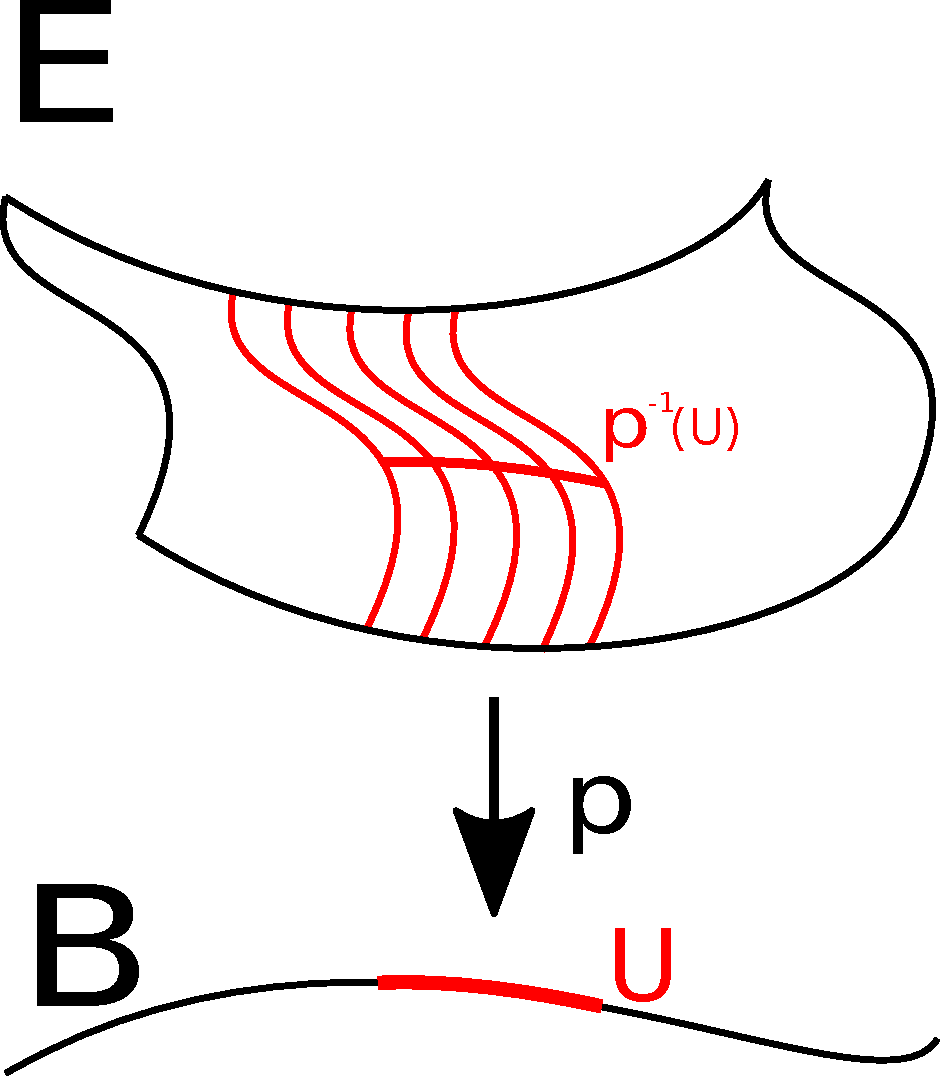
\includegraphics[scale=0.3]{fibrado.pdf}
        \caption{Illustration of the local triviality of a vector bundle.}
    \end{figure}
    
    Note that every vector bundle $\xi=(E,p,B)$ admits a section $s:B\to E$, called the zero section\index{section!zero}, defined by 
    $s(b)=0\in p^{-1}(b)$.
    
    \begin{defi}\label{fv_iso}
        We say that two $\R^{n}-$vector bundles $\xi=(E,p,B)$ and $\xi'=(E',q,B)$ are isomorphic\index{isomorphism}, denoted by 
        $\xi\cong\xi'$, if there exists a homeomorphism $h:E\to E'$ such that $q\circ h=p$ and $h|_{p^{-1}(b)}:p^{-1}(b)\to q^{-1}(b)$ is a 
        vector space isomorphism\index{isomorphism!vector space} for every $b\in B$.
    \end{defi}
    
    Now, let us recall how to specifically define the tangent and normal vector bundles of a smooth manifold and of a smooth embedding, 
    respectively.
    
    Consider $M^{m}$ a smooth $m$-dimensional manifold and define $TM=\ds\bigcup_{b\in M}\{b\}\times T_{b}M$, recalling that $T_{b}M$ is the 
    tangent space of $M$ at $b$.
    
    Thus, $\tau(M)=(TM,p_{1},M)$ defines an $\R^{m}$-vector bundle, where the fiber over $b\in M$ is $p_{1}^{-1}(b)=\{b\}\times T_{b}M$.
    
    \begin{defi}\label{defi_fvt}
        $\tau(M)$ is called the tangent vector bundle\index{bundle!vector!tangent} of the smooth manifold\index{manifold!smooth} $M$.
    \end{defi}
    
    Recall that an immersion\index{immersion} $i:N^{n}\to M^{n+k}$ is a map between smooth manifolds such that its differential 
    $d_{b}i:T_{b}N\to T_{i(b)}M$ is an injective linear transformation for every $b\in N$.

    In this context, we can ensure that $d_{b}i(T_{b}N)$ is a linear subspace of $T_{i(b)}M$. Thus, the set 
    $E(i)=\{ (b,v)\in N\times T_{i(b)}M \ : \ v\in [d_{b}i(T_{b}N)]^{\perp}\subset T_{i(b)}M \}$ is well defined.
    
    Therefore, $\nu(i)=(E(i),p_{1},N)$ is an $\R^{k}$-vector bundle, where the fiber over $b\in N$ is given by 
    $p_{1}^{-1}(b)=\{b\}\times [d_{b}i(T_{b}N)]^{\perp}$.
    
    \begin{defi}\label{defi_fvn}
        $\nu(i)$ is called the normal vector bundle\index{vector bundle!normal} of the immersion $i:N\to M$.
    \end{defi}
    
    Note that the normal vector bundle can also be defined for a smooth embedding\index{embedding!smooth}, since every smooth embedding is 
    both a topological embedding\index{embedding!topological} and an immersion\index{immersion}.
    
    To conclude the topics about vector bundles, let us present the following relation between the tangent and normal vector bundles of a 
    smooth embedding between smooth manifolds\index{manifold!smooth}, whose proof can be found in 
    (\cite{milnor_1}, Corollaries 3.4 and 3.5, pp. 30–31).
    
    \begin{teo}\label{dualidade_whitney_vet}
        If $i:N^{n}\to M^{n+k}$ is a smooth embedding between smooth manifolds, then:
        $$ \tau(N)\oplus\nu(i)\cong i^{*}(\tau(M)) $$
    \end{teo}



    \section{Fibration and Pair Fibration}\label{secao_fib_pares}

    \

    In this section, we will define the concept of pair fibration\index{fibration!of pairs}, also developed by Fadell in \cite{fadell_1}, 
    which can be considered as a fibration\index{fibration} whose total space is a pair of topological spaces.

    The definition of pair fibration will be necessary when we define generalized bundles\index{bundle!generalized} in the next section. We 
    will use the properties developed in this section as an intermediate step in the proofs of results involving generalized bundles.
    
    Except for Example \ref{pf_fv}, all the results presented throughout this section can be found, with few details, in \cite{fadell_1} and 
    \cite{brown}.
    
    \begin{defi}\label{PLH}
        We say that a map $p:E\to B$ satisfies the homotopy lifting property\index{homotopy lifting property} (HLP) over a topological space 
        $X$ if, for any maps $h:X\to E$ and $H:X\times I\to B$ such that $H(\_,0)=p\circ h$, there exists a continuous map 
        $\wt{H}:X\times I\to E$ such that $\wt{H}(\_,0)=h$ and $p\circ\wt{H}=H$. In this case, we have the following commutative diagram: 
        $$ \xymatrix @C=0.5cm {
            X\times \{ 0 \} \ar[rrr]^-{h} \ar@{^(->}[dd] &&& E \ar[dd]^-{p} \\
            &&& \\
            X\times I \ar[rrr]^-{H} \ar[rrruu]^-{\wt{H}} &&& B
        }$$
    \end{defi}

    \
    
    \begin{defi}
        A onto map $p:E\to B$ is said to be a fibration\index{fibration} if $p$ satisfies the HLP over any topological space $X$.
    
        In this context, we call the triple $\mathcal{F}=(E,p,B)$ a fibration over a base space $B$, with total space $E$ and fiber 
        $F=p^{-1}(b)$ over $b\in B$. We say that a map $s:B\to E$ is a section\index{section} of $\mathcal{F}$ if $p\circ s=1$.
    \end{defi}
    
    \begin{defi}{\bf (Pair Fibration)}\label{defi_par-fib}
        Let $p:E\to B$ be a onto map and $E_{0}\subset E$. We call $(\mathcal{F},\mathcal{F}_{0})=(E,E_{0},p,B)$ a pair 
        fibration\index{fibration!of pairs} if, for any topological space $X$ and any maps $h:X\to E$ and $H:X\times I\to B$ such that 
        $H(\_,0)=p\circ h$, there exists a continuous map $\wt{H}:X\times I\to E$ such that $\wt{H}(\_,0)=h$, $p\circ\wt{H}=H$, and if 
        $x_{0}\in X$ is such that $h(x_{0})\in E_{0}$, then $\wt{H}(x_{0},\_)\in E_{0}$.
    
        In this context, we say that $(\mathcal{F},\mathcal{F}_{0})$ is a pair fibration over a base space $B$, with total space $(E,E_{0})$ 
        and fiber $(F,F_{0})=(p^{-1}(b),p^{-1}(b)\cap E_{0})$ over $b\in B$.
    
        We also say that a map $s:B\to E$ is a section\index{section} of $(\mathcal{F},\mathcal{F}_{0})$ if $p\circ s=1$.
    \end{defi}
    
    Note that Definition \ref{defi_par-fib} guarantees that $\mathcal{F}=(E,p,B)$ and $\mathcal{F}_{0}=(E_{0},p_{0}=p_{|E_{0}},B)$ are 
    fibrations.
    
    Historically, the concept of fibration coincides with the concept of "fiber space\index{fiber space}" given by Hurewicz in 
    (\cite{hurewicz}, Section 1, p. 956), as also shown in (\cite{hurewicz}, Section 2, p. 957). Thus, the concept of pair fibration 
    coincides with the so-called "fibered pair\index{fibered pair}" given by Fadell in (\cite{fadell_1}, Definition 2.3, p. 489), as shown 
    in (\cite{brown}, Lemma 1.4, p. 183).
    
    As the simplest example of a pair fibration, we have the expected one:

    \begin{ex}\label{pf_trivial}
        Considering $B$ an arbitrary topological space, we obtain a pair fibration 
        $(\varepsilon_{B}^{n},\varepsilon_{B}^{n,0})=(B\times\R^{n},B\times(\R^{n}-\{ 0 \}),p_{1},B)$ with fiber homeomorphic to 
        $(\R^{n},\R^{n}-\{ 0 \})$.
    \end{ex}
    \begin{proof}

        \
    
        Initially, consider $X$ any topological space and maps $h:X\to B\times\R^{n}$ and $H:X\times I\to B$ such that the following 
        commutative diagram is obtained:
        $$\xymatrix @C=0.5cm {
            X\times\{ 0 \} \ar[rrr]^-{h} \ar@{^(->}[dd] &&& B\times\R^{n} \ar[dd]^-{p_{1}} \\
            &&& \\
            X\times I \ar[rrr]^-{H} &&& B
        }$$

        \
        
        Since $h=(h_{1},h_{2})$, define $\wt{H}:X\times I\to B\times\R^{n}$ by $\wt{H}(x,t)=(H(x,t),h_{2}(x))$. Clearly, $\wt{H}$ is 
        continuous, $p_{1}\circ\wt{H}=H$, and $\wt{H}(\_,0)=h$, since $H(\_,0)=h_{1}$. Furthermore, if $x_{0}\in X$ is such that 
        $h(x_{0})\in B\times (\R^{n}-\{ 0 \})$, then $h_{2}(x_{0})\in \R^{n}-\{ 0 \}$, and thus, 
        $\wt{H}(x_{0},\_)\in B\times(\R^{n}-\{ 0 \})$.
        
        Finally, given $(F,F_{0})$ the fiber of $(\mathcal{F},\mathcal{F}_{0})$ over any $b\in B$, we have:

        \
        
        $\begin{array}{rl}
            F \ = & p_{1}^{-1}(b) \\
            = & \{ b \}\times\R^{n} \\
            \approx & \R^{n}
        \end{array}$
        
        \
        
        \
        
        $\begin{array}{rl}
            F_{0} \ = & p_{1}^{-1}(b)\cap [B\times(\R^{n}-\{ 0 \})] \\
            = & [\{ b \}\times\R^{n}]\cap [B\times(\R^{n}-\{ 0 \})] \\
            = & \{ b \}\times(\R^{n}-\{ 0 \}) \\
            \approx & \R^{n}-\{ 0 \}
        \end{array}$ 

        \
        
        Thus, $(\varepsilon_{B}^{n},\varepsilon_{B}^{n,0})$ is indeed a pair fibration.
    
    \end{proof}
    
    Note that Example \ref{pf_trivial} also remains valid if we replace $\R^{n}$ with any topological space $F$ and $\R^{n}-\{ 0 \}$ with 
    any subspace $F_{0}\subset F$. However, in this case, the fiber would be homeomorphic to the pair $(F,F_{0})$.
    
    Next, we will present an alternative way of constructing pair fibrations, whose proof can be found in (\cite{allaud}, Theorem 2.5, p.241).
    
    \begin{teo}\label{teo_hurewicz}
        Let $p:E\to B$ be a onto map with $B$ paracompact, and pairs $(F,F_{0})$ and $(E,E_{0})$. If there exists an open covering 
        $\mathcal{U}$ of $B$ such that, for each $U\in\mathcal{U}$, there exists a homeomorphism 
        $h_{U}:(U\times F,U\times F_{0})\to (p^{-1}(U),p^{-1}(U)\cap E_{0})$ such that $p\circ h_{U}=p_{1}$, then $(E,E_{0},p,B)$ is a pair 
        fibration.
    \end{teo}

    Theorem \ref{teo_hurewicz} can be considered the version of the Hurewicz Uniformization Theorem\index{theorem!Hurewicz Uniformization 
    Theorem}\footnote{For more details on the Hurewicz Uniformization Theorem, see \cite{hurewicz}.} for fibrations of pairs.

    Thus, we can obtain the following:
    
    \begin{ex}\label{pf_fv}
        Every $\R^{n}$-vector bundle\index{vector bundle}, over a paracompact base, can be associated with a pair 
        fibration\index{fibration!of pairs}, whose fiber is homeomorphic to the pair $(\R^{n},\R^{n}-\{ 0 \})$.
    \end{ex}
    \begin{proof}
    
    \
    
    First, consider $\xi=(E,p,B)$ an $\R^{n}$-vector bundle over a paracompact $B$. By Definition \ref{fv_defi}, we know that there exists an 
    open cover $\mathcal{U}$ of $B$ such that, for every $U\in\mathcal{U}$, there exists a homeomorphism $h_{U}:U\times\R^{n}\to p^{-1}(U)$ 
    satisfying $p\circ h_{U}=p_{1}$.
    
    Denoting by $s:B\to E$ the zero section\index{zero section} of $\xi$ and $E_{0}=E-s(B)$, it is clear that we can consider 
    $h_{U}:(U\times\R^{n},U\times(\R^{n}-\{ 0 \}))\to (p^{-1}(U),p^{-1}(U)\cap E_{0})$ as a homeomorphism of pairs.
    
    Therefore, it follows from Theorem \ref{teo_hurewicz} that $(\xi,\xi_{0})=(E,E_{0},p,B)$ is a pair fibration.
    
    \end{proof}
    
    Now, as the final part of this section, let us see how to construct some pair fibrations from others.
    
    \begin{lem}\label{pf_restricao}
        Let $(\mathcal{F},\mathcal{F}_{0})=(E,E_{0},p,B)$ be a pair fibration and $U\subset B$ any subset. Then, 
        $(\mathcal{F},\mathcal{F}_{0})_{|U}=(p^{-1}(U),p^{-1}(U)\cap E_{0},p_{|p^{-1}(U)},U)$ will be a pair 
        fibration\index{fibration!of pairs} with fiber equal to the fiber of $(\mathcal{F},\mathcal{F}_{0})$.
    \end{lem}
    \begin{proof}
    
    \
    
    First, denote $q=p_{|p^{-1}(U)}$ and consider $X$ an arbitrary topological space and maps $h:X\to p^{-1}(U)$ and $H:X\times I\to U$ such 
    that the following diagram commutes:
    $$ \xymatrix @C=0.5cm {
        X\times\{ 0 \} \ar[rrr]^-{h} \ar@{^(->}[dd] &&& p^{-1}(U) \ar[dd]^-{q} \\
        &&& \\
        X\times I \ar[rrr]^-{H} &&& U 
    }$$
    
    Since $Im(H)\subset U\subset B$ and $(\mathcal{F},\mathcal{F}_{0})$ is a pair fibration, there exists a map $\wt{H}:X\times I\to E$ such 
    that $p\circ\wt{H}=H$ and $\wt{H}(\_,0)=h$. On the other hand, $Im(p\circ\wt{H})=Im(H)\subset U$, and thus $Im(\wt{H})\subset p^{-1}(U)$.
    
    Moreover, if $x_{0}\in X$ is such that $h(x_{0})\in E_{0}$, then $\wt{H}(x_{0},\_)\in E_{0}$. That is, if 
    $h(x_{0})\in p^{-1}(U)\cap E_{0}$, then $\wt{H}(x_{0},\_)\in p^{-1}(U)\cap E_{0}$.
    
    Finally, letting $(F',F'_{0})$ and $(F,F_{0})$ be the fibers of $(\mathcal{F},\mathcal{F}_{0})_{|U}$ and $(\mathcal{F},\mathcal{F}_{0})$, 
    respectively, over the same $b\in U$, we have:

    \
    
    $\begin{array}{rl}
        F' \ = & q^{-1}(b) \\
        = & p^{-1}(b)\cap p^{-1}(U) \\
        = & p^{-1}(b) \\
        = & F
    \end{array}$

    \

    \

    $\begin{array}{rl}
        F'_{0} \ = & q^{-1}(b)\bigcap [p^{-1}(U)\cap E_{0}] \\
        = & p^{-1}(b)\bigcap [p^{-1}(U)\cap E_{0}] \\
        = & p^{-1}(b)\cap E_{0} \\
        = & F_{0}
    \end{array}$

    \
    
    Therefore, $(\mathcal{F},\mathcal{F}_{0})_{|U}$ is a pair fibration.
    
    \end{proof}

    \begin{lem}\label{pf_pullback}
        Let $(\mathcal{F},\mathcal{F}_{0})=(E,E_{0},p,B)$ be a pair fibration and $f:B'\to B$ a map. Then, 
        $f^{*}(\mathcal{F},\mathcal{F}_{0})=(f^{*}E,f^{*}E_{0},p_{1},B')$ is also a pair fibration\index{fibration!of pairs} with fiber 
        homeomorphic to the fiber of $(\mathcal{F},\mathcal{F}_{0})$, where:
        
        \begin{enumerate}
            \item $f^{*}E=\{ (b',e)\in B'\times E \ : \ f(b')=p(e) \}$
            \item $f^{*}E_{0}=\{ (b',e)\in f^{*}E \ : \ e\in E_{0} \}$
        \end{enumerate}
    \end{lem}
    
    \begin{proof}
    
    \

        At first, let $X$ be any topological space and $h:X\to f^{*}E$ and $H:X\times I\to B'$ maps such that the following diagram commutes:
        $$\xymatrix @C=0.5cm {
            X\times\{ 0 \} \ar[rrr]^-{h} \ar@{^(->}[dd] &&& f^{*}E \ar[rrr]^-{p_{2}} \ar[dd]^-{p_{1}} &&& E \ar[dd]^-{p} \\
            &&& &&& \\
            X\times I \ar[rrr]^-{H} &&& B' \ar[rrr]^-{f} &&& B
        }$$

        \
        
        Denoting $g=p_{2}\circ h:X\to E$ and $G=f\circ H:X\times I\to B$, since the diagram above commutes and 
        $(\mathcal{F},\mathcal{F}_{0})$ is a pair fibration, there exists $\widetilde{G}:X\times I\to E$ such that 
        $p\circ\widetilde{G}=G$, $\widetilde{G}(\_,0)=g$, and if $x_{0}\in X$ is such that $g(x_{0})\in E_{0}$, then 
        $\widetilde{G}(x_{0},\_)\in E_{0}$.
        
        On the other hand, it is clear that $\widetilde{H}=(H,\widetilde{G}):X\times I\to f^{*}E$ is well-defined, since 
        $f\circ H=G=p\circ\widetilde{G}$. Moreover, $p_{1}\circ\widetilde{H}=H$ and $\widetilde{H}(\_,0)=h$, since $H(\_,0)=p_{1}\circ h$ 
        and $\widetilde{G}(\_,0)=p_{2}\circ h$.
        
        Thus, if $x_{0}\in X$ is such that $h(x_{0})\in f^{*}E_{0}$, then $g(x_{0})=p_{2}\circ h(x_{0})\in E_{0}$, and consequently, 
        $\widetilde{G}(x_{0},\_)\in E_{0}$. Therefore, $\widetilde{H}(x_{0},\_)\in f^{*}E_{0}$.
        
        Finally, if $(F',F'_{0})$ and $(F,F_{0})$ are fibers of $f^{*}(\mathcal{F},\mathcal{F}_{0})$ and $(\mathcal{F},\mathcal{F}_{0})$ 
        over $b'_{0}\in B'$ and $f(b'_{0})\in B$, respectively, then:

        \
        
        $\begin{array}{rl}
            F' = & p_{1}^{-1}(b'_{0}) \\
            = & \{ (b',e)\in f^{*}E \ : \ b'=p_{1}(b',e)=b'_{0} \} \\
            = & \{ (b'_{0},e)\in B'\times E \ : \ f(b'_{0})=p(e) \} \\
            = & \{ (b'_{0},e)\in B'\times E \ : \ e\in p^{-1}(f(b'_{0})) \} \\
            = & \{ b'_{0} \}\times p^{-1}(f(b'_{0})) \\
            = & \{ b'_{0} \}\times F \\
            \approx & F
        \end{array}$
        
        \

        \
        
        $\begin{array}{rl}
            F'_{0} = & p_{1}^{-1}(b'_{0})\cap f^{*}E_{0} \\
            = & (\{ b'_{0} \}\times F)\cap f^{*}E_{0} \\
            = & \{ b'_{0} \}\times (F\cap E_{0}) \\
            = & \{ b'_{0} \}\times F_{0} \\
            \approx & F_{0}
        \end{array}$
        
        \
        
        Therefore, $f^{*}(\mathcal{F},\mathcal{F}_{0})$ is indeed a pair fibration.
    \end{proof}

    \begin{lem}\label{pf_produto}
        Let $(\mathcal{F},\mathcal{F}_{0})=(E,E_{0},p,B)$ and $(\mathcal{F'},\mathcal{F'}_{0})=(E',E'_{0},q,B')$ be two pair fibrations. 
        Then, $(\mathcal{F},\mathcal{F}_{0})\times(\mathcal{F'},\mathcal{F'}_{0})=(E'',E''_{0},r,B'')$ will be a pair 
        fibration\index{fibration!of pairs} with fiber equal to the product of the fibers of $(\mathcal{F},\mathcal{F}_{0})$ and 
        $(\mathcal{F'},\mathcal{F'}_{0})$, where:
        
        \begin{enumerate}
            \item $E''=E\times E'$
            \item $E''_{0}=(E\times E'_{0})\cup (E_{0}\times E')$
            \item $r=p\times q$
        \end{enumerate}
        
    \end{lem}
    
    \begin{proof}
    
    \
    
        At first, let $X$ be any topological space and $h:X\to E''$ and $H:X\times I\to B''$ maps such that the following diagram commutes:
        $$\xymatrix @C=0.5cm {
            X\times\{ 0 \} \ar[rrr]^-{h} \ar@{^(->}[dd] &&& E'' \ar[dd]^-{r} \\
            &&& &&& \\
            X\times I \ar[rrr]^-{H} &&& B'' 
        }$$

        \
        
        Since $h=(h_{1},h_{2})$, $H=(H_{1},H_{2})$, and $H(\_,0)=r\circ h$, we have that $H_{1}(\_,0)=p\circ h_{1}$ and 
        $H_{2}(\_,0)=q\circ h_{2}$. As $(\mathcal{F},\mathcal{F}_{0})$ and $(\mathcal{F'},\mathcal{F'}_{0})$ are pair fibrations, there 
        exist maps $\wt{H_{1}}:X\times I\to E$ and $\wt{H_{2}}:X\times I\to E'$ such that $p\circ\wt{H_{1}}=H_{1}$, $q\circ\wt{H_{2}}=H_{2}$, 
        $\wt{H_{1}}(\_,0)=h_{1}$, $\wt{H_{2}}(\_,0)=h_{2}$, and if $x_{0}\in X$ is such that $h_{1}(x_{0})\in E_{0}$, then 
        $\wt{H_{1}}(x_{0},\_)\in E_{0}$. Moreover, if $x_{0}\in X$ is such that $h_{2}(x_{0})\in E'_{0}$, then 
        $\wt{H_{2}}(x_{0},\_)\in E'_{0}$.
        
        Thus, defining $\wt{H}=(\wt{H_{1}},\wt{H_{2}}):X\times I\to E''$, it is clear that $\wt{H}(\_,0)=h$ and $r\circ\wt{H}=H$. 
        Furthermore, if $x_{0}\in X$ is such that $h(x_{0})\in E''_{0}$, then $h_{1}(x_{0})\in E_{0}$ or $h_{2}(x_{0})\in E'_{0}$. 
        Hence, $\wt{H_{1}}(x_{0},\_)\in E_{0}$ or $\wt{H_{2}}(x_{0},\_)\in E'_{0}$, that is, $\wt{H}(x_{0},\_)\in E''_{0}$.
        
        Finally, consider, respectively, $(F,F_{0})$, $(F',F'_{0})$, and $(F'',F''_{0})$ the fibers of 
        $(\mathcal{F},\mathcal{F}_{0})$, $(\mathcal{F'},\mathcal{F'}_{0})$, and 
        $(\mathcal{F},\mathcal{F}_{0})\times (\mathcal{F'},\mathcal{F'}_{0})$ over $b\in B$, $b'\in B'$, and $(b,b')\in B''$. Then:

        \
        
        $\begin{array}{rl}
            F'' \ = & r^{-1}(b,b') \\
            = & p^{-1}(b)\times q^{-1}(b') \\
            = & F\times F'
        \end{array}$
        
        \

        \

        $\begin{array}{rl}
            F''_{0} \ = & r^{-1}(b,b')\cap E''_{0} \\
            = & (F\times F')\bigcap [(E\times E'_{0})\cup (E_{0}\times E')] \\
            = & [(F\times F')\cap (E\times E'_{0})]\bigcup [(F\times F')\cap (E_{0}\times E')] \\
            = & [F\times (F'\cap E'_{0})]\bigcup [(F\cap E_{0})\times F'] \\
            = & (F\times F'_{0})\cup (F_{0}\times F')
        \end{array}$
        
        \
        
        Therefore, $(\mathcal{F},\mathcal{F}_{0})\times (\mathcal{F'},\mathcal{F'}_{0})$ will be a pair fibration.
        
    \end{proof}

    

    \section{Generalized Bundle}\label{secao_fib_gener}

    \

    In this section, we will present the tool developed by Fadell in \cite{fadell_1} that allows us to generalize 
    tangent\index{vector bundle!tangent} and normal\index{vector bundle!normal} vector bundles of smooth manifolds\index{manifold!smooth} to 
    topological manifolds\index{manifold!topological}. This tool is called the generalized bundle.

    Except for examples \ref{fht_sobre_ponto} and \ref{fht_fv}, lemmas \ref{iso_homot} and \ref{iso_homot_2}, and propositions 
    \ref{iso_fv_fht}, \ref{iso_homeo}, \ref{fht_tang_cart}, and \ref{iso_merg_lf_2}, all other results were taken from \cite{fadell_1}. 
    However, we will provide more detailed proofs of these results here.
    
    \begin{defi}{\bf (Generalized Bundle)}\label{defi_fib_gen}
        A pair fibration\index{pair fibration} $(\mathcal{F},\mathcal{F}_{0})=(E,E_{0},p,B)$ is said to be an $\R^{n}$-generalized 
        bundle\index{generalized bundle} if:
    
        \begin{enumerate}
            \item There exists a section\index{section} $s:B\to E$ of $(\mathcal{F},\mathcal{F}_{0})$ such that $E_{0}$ is realized, i.e., 
            $E_{0}=E-s(B)$.
            \item Every fiber $(F,F_{0})$ of $(\mathcal{F},\mathcal{F}_{0})$ satisfies $(F,F_{0})\sim (\R^{n},\R^{n}-\{ 0 \})$.
        \end{enumerate}
    \end{defi}
    
    \begin{ex}\label{fht_trivial}
        The pair fibration $(\varepsilon^{n}_{B},\varepsilon^{n,0}_{B})$ is an $\R^{n}-$generalized bundle.
    \end{ex}
    \begin{proof}
        
        \
    
        Since Example \ref{pf_trivial} already shows that $(\varepsilon^{n}_{B},\varepsilon^{n,0}_{B})$ is a pair fibration with a fiber 
        homeomorphic to the pair $(\R^{n},\R^{n}-\{ 0 \})$, it is enough to define a section of $(\varepsilon^{n}_{B},\varepsilon^{n,0}_{B})$ 
        that realizes $B\times(\R^{n}-\{ 0 \})$.
    
        Note that $s:B\to B\times\R^{n}$ defined by $s(b)=(b,0)$ is the required section.
    
        Therefore, $(\varepsilon^{n}_{B},\varepsilon^{n,0}_{B})$ is an $\R^{n}-$generalized bundle.
    
    \end{proof}
    
    \begin{lem}\label{fht_restricao}
        If $(\mathcal{F},\mathcal{F}_{0})$ is an $\R^{n}-$generalized bundle\index{generalized bundle} over $B$, then 
        $(\mathcal{F},\mathcal{F}_{0})_{|U}$ will also be an $\R^{n}-$generalized bundle for any $U\subset B$.
    \end{lem}
    \begin{proof}
        
        \
    
        From Lemma \ref{pf_restricao}, we already know that if $(\mathcal{F},\mathcal{F}_{0})$ is a pair fibration\index{pair fibration}, 
        then for any arbitrary $U\subset B$, $(\mathcal{F},\mathcal{F}_{0})_{|U}$ will also be a pair fibration with fiber equal to the fiber 
        of $(\mathcal{F},\mathcal{F}_{0})$.
        
        Thus, let $(\mathcal{F},\mathcal{F}_{0})=(E,E_{0},p,B)$ and 
        $(\mathcal{F},\mathcal{F}_{0})_{|U}=(p^{-1}(U),p^{-1}(U)\cap E_{0},p_{|p^{-1}(U)},U)$. It is enough to find a 
        section\index{section} of $(\mathcal{F},\mathcal{F}_{0})_{|U}$ that realizes $p^{-1}(U)\cap E_{0}$.
    
        Since $(\mathcal{F},\mathcal{F}_{0})$ is an $\R^{n}-$generalized bundle, there exists a section $s:B\to E$ of 
        $(\mathcal{F},\mathcal{F}_{0})$ that realizes $E_{0}$.
        
        Now, define $s'=s_{|U}:U\to p^{-1}(U)$. Clearly, $Im(s')\subset p^{-1}(U)$ because $p\circ s(U)=U$. Furthermore, we have:

        \
    
        $\begin{array}{rl}
            p^{-1}(U)\cap E_{0} = & p^{-1}(U)\bigcap [E-s(B)] \\
            = & [p^{-1}(U)\cap E]-[p^{-1}(U)\cap s(B)] \\
            = & p^{-1}(U)-s(U) \\
            = & p^{-1}(U)-s'(U)
        \end{array}$

        \
    
        Therefore, $(\mathcal{F},\mathcal{F}_{0})_{|U}$ will also be an $\R^{n}-$generalized bundle for all $U\subset B$.
    
    \end{proof}
    
    Following the notation of Lemma \ref{fht_restricao}, if $(\mathcal{F},\mathcal{F}_{0})$ is an $\R^{n}-$generalized bundle, we call 
    $(\mathcal{F},\mathcal{F}_{0})_{|U}$ the restriction of the $\R^{n}-$generalized bundle\index{generalized bundle!restriction} of 
    $(\mathcal{F},\mathcal{F}_{0})$ to $U\subset B$.
    
    \begin{defi}
        Let $(\mathcal{F},\mathcal{F}_{0})=(E,E_{0},p,B)$ and $(\mathcal{F'},\mathcal{F'}_{0})=(E',E'_{0},q,B)$ be $\R^{n}$-generalized 
        bundles over the same base. We call $\phi:(\mathcal{F},\mathcal{F}_{0})\to (\mathcal{F'},\mathcal{F'}_{0})$ a fiber 
        map\index{fiber map} if $\phi:(E,E_{0})\to (E',E'_{0})$ is a map that preserves the fibers, i.e., $q\circ\phi=p$.
    \end{defi}

    \begin{defi}\label{defi_iso_homot}
        We say that two $\R^{n}-$generalized bundles over the same base, $(\mathcal{F},\mathcal{F}_{0})=(E,E_{0},p,B)$ and 
        $(\mathcal{F'},\mathcal{F'}_{0})=(E',E'_{0},q,B)$, are homotopically isomorphic if there exist fiber maps 
        $\phi:(\mathcal{F},\mathcal{F}_{0})\rightleftarrows (\mathcal{F'},\mathcal{F'}_{0}):\psi$ and $H:(E,E_{0})\times I\to (E,E_{0})$ and 
        $G:(E',E'_{0})\times I\to (E',E'_{0})$ homotopies such that:
        
        \

        $\begin{array}{lcccl}
            1. \ H(\_,0)=\psi\circ\phi            & & & & 4. \ G(\_,0)=\phi\circ\psi \\
            2. \ H(\_,1)=1                        & & & & 5. \ G(\_,1)=1 \\
            3. \ p\circ H(\_,t)=p, \forall t\in I & & & & 6. \ q\circ G(\_,t)=q, \forall t\in I
        \end{array}$

        \
    
        The homotopy isomorphism\index{isomorphism!homotopy}, defined above, will be denoted by 
        $(\mathcal{F},\mathcal{F}_{0})\sim_{f} (\mathcal{F'},\mathcal{F'}_{0})$.
    \end{defi}
    
        The notion of homotopy isomorphism, as given in the definition above, coincides with the concept of "fiber homotopy 
        equivalence\index{fiber homotopy equivalence}" given by Fadell in (\cite{fadell_1}, Definition 2.4, p. 489).
    
    \begin{defi}
        We call a $\R^{n}-$generalized bundle $(\mathcal{F},\mathcal{F}_{0})$, over $B$, locally trivial\index{locally trivial} if there 
        exists an open cover $\mathcal{U}$ of $B$ such that 
        $(\mathcal{F},\mathcal{F}_{0})_{|U}\sim_{f} (\varepsilon^{n}_{U},\varepsilon^{n,0}_{U})$, for every $U\in\mathcal{U}$. In particular, 
        $(\mathcal{F},\mathcal{F}_{0})$ will be called a trivial $\R^{n}-$generalized bundle\index{fiber bundle!generalized!trivial} if 
        $(\mathcal{F},\mathcal{F}_{0})\sim_{f} (\varepsilon^{n}_{B},\varepsilon^{n,0}_{B})$.
    \end{defi}
    
    \begin{ex}\label{fht_sobre_ponto}
        Every $\R^{n}-$generalized bundle over a point is trivial.
    \end{ex}
    \begin{proof}
    
        \
    
        Let us denote by $(\mathcal{F},\mathcal{F}_{0})=(E,E_{0},p,\{ * \})$ a $\R^{n}-$generalized bundle whose base space consists of only 
        one point.
    
        Thus, it is clear that $(E,E_{0})=(p^{-1}(*),p^{-1}(*)\cap E_{0})\sim (\R^{n},\R^{n}-\{0 \})$, that is, there exist fiber maps 
        $\phi:(E,E_{0})\rightleftarrows (\R^{n},\R^{n}-\{ 0 \}):\psi$ and homotopies $H:(E,E_{0})\times I\to (E,E_{0})$ and 
        $G:(\R^{n},\R^{n}-\{0 \})\times I\to (\R^{n},\R^{n}-\{0 \})$ such that $H(\_,0)=\psi\circ\phi$, $H(\_,1)=1$, $G(\_,0)=\phi\circ\psi$ 
        and $G(\_,1)=1$.
    
        Thus, the following fiber maps\index{fiber map} and homotopies are well-defined:
    
        \begin{enumerate}
            \item $\overline{\phi}:(E,E_{0})\rightleftarrows (\{ * \}\times\R^{n},\{ * \}\times\R^{n}-\{0 \}):\overline{\psi}$ \\
            $ \overline{\phi}(e)=(*,\phi(e)) $ \\
            $ \overline{\psi}(*,x)=\psi(x) $
            \item $\overline{H}:(E,E_{0})\times I\to (E,E_{0})$ \\
            $ \overline{H}(e,t)=H(e,t) $
            \item $\overline{G}:(\{ * \}\times\R^{n},\{ * \}\times\R^{n}-\{0 \})\times I \to (\{ * \}\times\R^{n},\{ * \}\times\R^{n}-\{0 \})$ \\
            $ \overline{G}((*,x),t)=(*,G(x,t)) $
        \end{enumerate}
    
        It is clear that $\overline{H}(\_,1)=1$, $\overline{G}(\_,1)=1$, $p\circ\overline{H}(\_,t)=p$ and $p_{1}\circ\overline{G}(\_,t)=p_{1}$ 
        for any $t\in I$. Also:

        \
    
        $\begin{array}{rl}
            \forall e\in E, \ \overline{H}(e,0) \ = & H(e,0) \\
            = & \psi\circ\phi(e) \\
            = & \overline{\psi}(*,\phi(e)) \\
            = & \overline{\psi}\circ\overline{\phi}(e)
        \end{array}$

        \

        \

        $\begin{array}{rl}
            \forall x\in \R^{n}, \ \overline{G}((*,x),0) \ = & (*,G(x,0)) \\
            = & (*,\phi\circ\psi(x)) \\
            = & \overline{\phi}(\psi(x)) \\
            = & \overline{\phi}\circ\overline{\psi}(*,x)
        \end{array}$

        \
    
        Therefore, $(\mathcal{F},\mathcal{F}_{0})\sim_{f}(\varepsilon^{n}_{\{ * \}},\varepsilon^{n,0}_{\{ * \}})$.
    
    \end{proof}

    Regarding specific conditions, the homotopy isomorphism\index{isomorphism!homotopy} can be guaranteed more simply, as follows:

    \begin{lem}\label{iso_homot}
        Let $(\mathcal{F},\mathcal{F}_{0})$ and $(\mathcal{F'},\mathcal{F'}_{0})$ be two $\R^{n}-$generalized bundles, over the same base. 
        If $\phi:(\mathcal{F},\mathcal{F}_{0})\to (\mathcal{F'},\mathcal{F'}_{0})$ is a fiber map\index{map!fiber} such that $\phi$ is a 
        homeomorphism, then $(\mathcal{F},\mathcal{F}_{0})\sim_{f} (\mathcal{F'},\mathcal{F'}_{0})$.
    \end{lem}
    \begin{proof}
    
        \
        
        Initially, since $\phi$ is a homeomorphism and $q\circ\phi=p$, it follows that $p\circ\phi^{-1}=q$, that is, 
        $\phi^{-1}:(\mathcal{F},\mathcal{F}_{0})\to (\mathcal{F'},\mathcal{F'}_{0})$ is also a fiber map.
        
        Thus, it is evident that $(\mathcal{F},\mathcal{F}_{0})\sim_{f} (\mathcal{F},\mathcal{F}_{0})$, since it is sufficient to define 
        trivial homotopies for the conditions of homotopy isomorphism to be satisfied.
        
    \end{proof}
    
    In this way, using Lemma \ref{iso_homot} and the construction from Example \ref{pf_fv}, we obtain the following:
    
    \begin{ex}\label{fht_fv}
        If $\xi$ is an $\R^{n}-$vector bundle\index{bundle!vector} over a paracompact base, then its associated pair 
        fibration\index{fibration!pair} $(\xi,\xi_{0})$ will be a locally trivial $\R^{n}-$generalized bundle\index{bundle!generalized}.
    \end{ex}
    
    Therefore, we can consider that the notion of generalized bundles generalizes the concept of vector bundles. Thus, it is expected 
    that the isomorphism structure between vector bundles is preserved when passing to homotopy isomorphism\index{isomorphism!homotopy}, as 
    in the following:
    
    \begin{prop}\label{iso_fv_fht}
        Let $\xi$ and $\eta$ be two isomorphic $\R^{n}-$vector bundles\index{bundle!vector} over the same paracompact base. Then, their 
        respective associated $\R^{n}-$generalized bundles $(\xi,\xi_{0})$ and $(\eta,\eta_{0})$ are homotopy isomorphic.
    \end{prop}
    \begin{proof}
    
        \

        First, let $\xi=(E,p,B)\cong\eta=(E',q,B)$. Thus, by definition \ref{fv_iso}, there exists a homeomorphism $h:E\to E'$ such that 
        $q\circ h=p$ and $h_{|F}:F\to F'$ is a vector isomorphism\index{isomorphism!vector}, for any fibers $F$ and $F'$ of $\xi$ and $\eta$, 
        respectively, over the same $b\in B$.
        
        Let $s:B\to E$ and $s':B\to E'$ be the zero sections\index{section!zero} of $\xi$ and $\eta$, respectively, and consider 
        $E_{0}=E-s(B)$ and $E'_{0}=E'-s'(B)$. If we show that $h(E_{0})\subset E'_{0}$, then $h:(E,E_{0})\to (E',E'_{0})$ will be a 
        homeomorphism and a fiber map\index{map!fiber}, and thus, Lemma \ref{iso_homot} will guarantee that 
        $(\xi,\xi_{0})\sim_{f} (\eta,\eta_{0})$.
        
        To this end, note that:

        \
        
        $\begin{array}{rl}
            e\in E_{0} \Longrightarrow & e\in F=p^{-1}(p(e))\cong\R^{n} \text{ and } e\neq 0 \\
            \Longrightarrow & h(e)\in F'=q^{-1}(p(e))\cong\R^{n} \text{ and } h(e)\neq 0 \\
            \Longrightarrow & h(e)\in E'_{0}
        \end{array}$

        \
        
        Therefore, we conclude that $(\xi,\xi_{0})\sim_{f} (\eta,\eta_{0})$.
        
    \end{proof}
    
    \begin{lem}\label{fht_pullback}
        If $(\mathcal{F},\mathcal{F}_{0})$ is a $\R^{n}-$generalized bundle\index{bundle!generalized!trivial} over $B$ and $f:B'\to B$ is any 
        map, then $f^{*}(\mathcal{F},\mathcal{F}_{0})$ will also be a $\R^{n}-$generalized bundle. In particular, if 
        $(\mathcal{F},\mathcal{F}_{0})$ is trivial, then $f^{*}(\mathcal{F},\mathcal{F}_{0})$ will also be trivial.
    \end{lem}

    \begin{proof}

        \

        Due to lemma \ref{pf_pullback}, we already know that if $(\mathcal{F},\mathcal{F}_{0})$ is a pair fibration, then 
        $f^{*}(\mathcal{F},\mathcal{F}_{0})$ will be a pair fibration with fiber homeomorphic to the fiber of $(\mathcal{F},\mathcal{F}_{0})$. 
        Thus, denoting $(\mathcal{F},\mathcal{F}_{0})=(E,E_{0},p,B)$ and $f^{*}(\mathcal{F},\mathcal{F}_{0})=(f^{*}E,f^{*}E_{0},p_{1},B')$, 
        it is enough to show that there exists a section of $f^{*}(\mathcal{F},\mathcal{F}_{0})$ that realizes $f^{*}E_{0}$.
    
        To this end, since $(\mathcal{F},\mathcal{F}_{0})$ is a $\R^{n}-$generalized bundle, there exists a section $s:B\to E$ of 
        $(\mathcal{F},\mathcal{F}_{0})$ that realizes $E_{0}$. In this way, the section 
        $s':B'\to f^{*}E$ of $f^{*}(\mathcal{F},\mathcal{F}_{0})$ is well-defined, given by $s'(b')=(b',s(f(b')))$. Finally:

        \
        
        $\begin{array}{rl}
            f^{*}E_{0} \ = & [B'\times E_{0}]\bigcap f^{*}E \\
            = & [B'\times (E-s(B))]\bigcap f^{*}E \\
            = & [(B'\times E)-(B'\times s(B))]\bigcap f^{*}E \\
            = & [(B'\times E)\cap f^{*}E]-[(B'\times s(B))\cap f^{*}E] \\
            = & f^{*}E - \{ (b',s(b))\in B'\times s(B) \ : \ f(b')=p(s(b))=b \} \\
            = & f^{*}E - [B'\times s(f(B'))] \\
            = & f^{*}E - s'(B')
        \end{array}$
        
        \
    
        Therefore, $f^{*}(\mathcal{F},\mathcal{F}_{0})$ will be a $\R^{n}-$generalized bundle.
    
        Now, we need to show that if $(\mathcal{F},\mathcal{F}_{0})\sim_{f}(\varepsilon_{B}^{n},\varepsilon_{B}^{n,0})$, then 
        $f^{*}(\mathcal{F},\mathcal{F}_{0})\sim_{f}(\varepsilon_{B'}^{n},\varepsilon_{B'}^{n,0})$. So, suppose there exist the following 
        fiber maps and homotopies satisfying the relations below:
    
        \begin{enumerate}
            \item $\phi:(E,E_{0})\rightleftarrows(B\times \R^{n},B\times (\R^{n}-\{ 0 \})):\psi$
            \item $H:(E,E_{0})\times I\to (E,E_{0})$
            \item $G:(B\times\R^{n},B\times(\R^{n}-\{ 0 \}))\times I\to (B\times\R^{n},B\times(\R^{n}-\{ 0 \}))$
            \item $\phi$, $\psi$, $H$, and $G$ satisfy:
            
                $\begin{array}{lcccl}
                    H(\_,0)=\psi\circ\phi            & & & & G(\_,0)=\phi\circ\psi \\
                    H(\_,1)=1                        & & & & G(\_,1)=1 \\
                    p\circ H(\_,t)=p, \forall t\in I & & & & p_{1}\circ G(\_,t)=p_{1}, \forall t\in I
                \end{array}$
        \end{enumerate}

        \
    
        In this way, the following fiber maps and homotopies are well-defined:
    
        \begin{enumerate}
            \item $\overline{\phi}:(f^{*}E,f^{*}E_{0})\rightleftarrows (B'\times \R^{n},B'\times (\R^{n}-\{ 0 \})):\overline{\psi}$ \\
            $ \overline{\phi}(b',e)=(b',p_{2}\circ\phi(e)) $ \\
            $ \overline{\psi}(b',x)=(b',\psi(f(b'),x)) $
            \item $\overline{H}:(f^{*}E,f^{*}E_{0})\times I\to (f^{*}E,f^{*}E_{0})$ \\
            $ \overline{H}((b',e),t)=(b',H(e,t)) $
            \item $\overline{G}:(B'\times \R^{n},B'\times (\R^{n}-\{ 0 \}))\times I\to (B'\times \R^{n},B'\times (\R^{n}-\{ 0 \}))$ \\
            $ \overline{G}((b',x),t)=(b',p_{2}\circ G((f(b'),x),t)) $
        \end{enumerate}

        \
    
        Let's show that $\overline{\phi}$, $\overline{\psi}$, $\overline{H}$, and $\overline{G}$ satisfy the conditions of definition 
        \ref{defi_iso_homot}. Indeed:
    
        \begin{enumerate}
            \item It is clear that $p_{1}\circ\overline{H}((\_,\_),t)=p_{1}$ and $p_{1}\circ\overline{G}((\_,\_),t)=p_{1}$ for all $t\in I$
            \item It is also clear that $\overline{H}((\_,\_),1)=1$ and $\overline{G}((\_,\_),1)=1$
            \item $\forall (b',e)\in f^{*}E$, \\
                   
                    $\begin{array}{rl}
                        \overline{H}((b',e),0) \ = & (b',H(e,0)) \\
                        = & (b',\psi\circ\phi(e)) \\
                        = & (b',\psi(p_{1}\circ\phi(e),p_{2}\circ\phi(e))) \\
                        = & (b',\psi(p(e),p_{2}\circ\phi(e))) \\
                        = & (b',\psi(f(b'),p_{2}\circ\phi(e))) \\
                        = & \overline{\psi}(b',p_{2}\circ\phi(e)) \\
                        = & \overline{\psi}\circ\overline{\phi}(b',e)
                    \end{array}$
            \item $\forall (b',x)\in B'\times\R^{n}$, \\
                    
                    $\begin{array}{rl}
                        \overline{G}((b',x),0) \ = & (b',p_{2}\circ G((f(b'),x),0)) \\
                        = & (b',p_{2}\circ\phi\circ\psi(f(b'),x)) \\
                        = & \overline{\phi}(b',\psi(f(b'),x)) \\
                        = & \overline{\phi}\circ\overline{\psi}(b',x)
                    \end{array}$
        \end{enumerate}
    
        \par Therefore, $f^{*}(\mathcal{F},\mathcal{F}_{0})\sim_{f}(\varepsilon_{B'}^{n},\varepsilon_{B'}^{n,0})$.
    
    \end{proof}

    Following the notation of Lemma \ref{fht_pullback}, given $(\mathcal{F},\mathcal{F}_{0})$ a $\R^{n}-$generalized bundle, we call 
    $f^{*}(\mathcal{F},\mathcal{F}_{0})$ the $\R^{n}-$generalized bundle pullback\index{fibration!generalized!pullback} of 
    $(\mathcal{F},\mathcal{F}_{0})$ by the map $f$.

    Now, let's look at some examples involving generalized fibration pullbacks.
    
    \begin{ex}\label{fht_pullback_ex1}
    Let $(\mathcal{F},\mathcal{F}_{0})$ and $(\mathcal{F'},\mathcal{F'}_{0})$ be two $\R^{n}-$generalized bundles, over the same base $B$, 
    such that $(\mathcal{F},\mathcal{F}_{0})\sim_{f} (\mathcal{F'},\mathcal{F'}_{0})$. Then, let $1:B\to B$ be the identity map, and we have 
    $(\mathcal{F},\mathcal{F}_{0})\sim_{f} 1^{*}(\mathcal{F'},\mathcal{F'}_{0})$.
    \end{ex}
    \begin{proof}

        \

        Initially, let us denote $(\mathcal{F},\mathcal{F}_{0})=(E,E_{0},p,B)$ and $(\mathcal{F'},\mathcal{F'}_{0})=(E',E'_{0},q,B)$. Since 
        $(\mathcal{F},\mathcal{F}_{0})\sim_{f} (\mathcal{F'},\mathcal{F'}_{0})$, there exist the following fiber maps and homotopies 
        satisfying the following relations:
        
        \begin{enumerate}
            \item $\phi:(E,E_{0}) \rightleftarrows (E',E'_{0}):\psi$
            \item $H:(E,E_{0}) \times I \to (E,E_{0})$
            \item $G:(E',E'_{0}) \times I \to (E',E'_{0})$
            \item $\phi$, $\psi$, $H$, and $G$ satisfy the following relations:
            
                $\begin{array}{lccl}
                    H(\_, 0) = \psi \circ \phi & & & G(\_, 0) = \phi \circ \psi \\
                    H(\_, 1) = 1 & & & G(\_, 1) = 1 \\
                    p \circ H(\_, t) = p, \ \forall t \in I & & & q \circ G(\_, t) = q, \ \forall t \in I
                \end{array}$
        \end{enumerate}
        
        \
        
        Recall that the $\R^{n}-$generalized bundle pullback\index{fibration!generalized!pullback} 
        $1^{*}(\mathcal{F'},\mathcal{F'}_{0})=(1^{*}E',1^{*}E'_{0},p_{1},B)$ is such that:
        $$1^{*}E'=\{ (b,e')\in B\times E' : b=q(e') \}$$
        $$1^{*}E'_{0}=\{ (b,e')\in 1^{*}E' : e'\in E'_{0} \}$$
        
        \

        So, the following fiber maps\index{map!fibration} and homotopies are 
        well-defined:
        
        \begin{enumerate}
            \item $\overline{\phi}:(E,E_{0})\rightleftarrows (1^{*}E',1^{*}E'_{0}):\overline{\psi}$ \\
            $\overline{\phi}(e)=(p(e),\phi(e))$ \\
            $\overline{\psi}(b,e')=\psi(e')$
            \item $\overline{H}:(E,E_{0})\times I\to (E,E_{0})$ \\
            $\overline{H}(e,t)=H(e,t)$
            \item $\overline{G}:(1^{*}E',1^{*}E'_{0})\times I\to (1^{*}E',1^{*}E'_{0})$ \\
            $\overline{G}((b,e'),t)=(b,G(e',t))$
        \end{enumerate}

        \
        
        Thus, it is clear that $\overline{H}(e,1)=e$, for all $e\in E$, and $p\circ\overline{H}(\_,t)=p$, for all $t\in I$, since $H$ has 
        these properties. Similarly, $\overline{G}((b,e'),1)=(b,e')$, for all $(b,e')\in 1^{*}E'$, and $p_{1}\circ\overline{G}(\_,t)=p_{1}$, 
        for all $t\in I$. Additionally, we have that:

        \
        
        $\begin{array}{rl}
            \forall e\in E, \ \overline{H}(e,0) = & H(e,0) \\
            = & \psi\circ\phi(e) \\
            = & \overline{\psi}(p(e),\phi(e)) \\
            = & \overline{\psi}\circ\overline{\phi}(e)
        \end{array}$

        \
 
        \

        $\begin{array}{rl}
            \forall (b,e')\in 1^{*}E', \ \overline{G}((b,e'),0) = & (b,G(e',0)) \\
            = & (b,\phi\circ\psi(e')) \\
            = & (q(e'),\phi\circ\psi(e')) \\
            = & (p\circ\psi(e'),\phi\circ\psi(e')) \\
            = & \overline{\phi}(\psi(e')) \\
            = & \overline{\phi}\circ\overline{\psi}(b,e')
        \end{array}$

        \
        
        Therefore, $(\mathcal{F},\mathcal{F}_{0})\sim_{f} 1^{*}(\mathcal{F'},\mathcal{F'}_{0})$.
    
    \end{proof}

    \begin{ex}\label{fht_pullback_ex2}
        Let $B$ be a topological space, $b_{0} \in B$ any point, and $c:B \to \{ b_{0} \}$ the constant map. Then, 
        $(\varepsilon^{n}_{B}, \varepsilon^{n,0}_{B}) \sim_{f} c^{*}(\varepsilon^{n}_{\{ b_{0} \}}, \varepsilon^{n,0}_{\{ b_{0} \}})$.
    \end{ex}
    \begin{proof}

        \
        
        Recall that 
        $c^{*}(\varepsilon^{n}_{\{ b_{0} \}}, \varepsilon^{n,0}_{\{ b_{0} \}}) = (c^{*}(\{ b_{0} \} \times \R^{n}), c^{*}[\{ b_{0} \} \times (\R^{n} - \{ 0 \})], p_{1}, B)$ 
        is the $\R^{n}$-generalized bundle pullback such that:

        \
        
        $\begin{array}{rl}
        c^{*}(\{ b_{0} \} \times \R^{n}) = & \{ (b, (b_{0}, x)) \in B \times (\{ b_{0} \} \times \R^{n}) : b_{0} = c(b) = p_{1}(b_{0}, x) = b_{0} \} \\
        = & B \times \{ b_{0} \} \times \R^{n}
        \end{array}$

        \

        \
        
        $c^{*}[\{ b_{0} \} \times (\R^{n} - \{ 0 \})] = B \times \{ b_{0} \} \times (\R^{n} - \{ 0 \})$

        \
        
        Thus, $\phi:(B \times \R^{n}, B \times (\R^{n} - \{ 0 \})) \rightleftarrows (B \times \{ b_{0} \} \times \R^{n}, B \times \{ b_{0} \} \times (\R^{n} - \{ 0 \})) : \psi$, 
        given by $\phi(b, x) = (b, b_{0}, x)$ and $\psi(b, b_{0}, x) = (b, x)$, respectively, are well-defined fiber maps, with $\phi$ being a 
        homeomorphism with inverse $\psi$.
        
        Therefore, by lemma \ref{iso_homot}, we conclude that 
        $(\varepsilon^{n}_{B}, \varepsilon^{n,0}_{B}) \sim_{f} c^{*}(\varepsilon^{n}_{\{ b_{0} \}}, \varepsilon^{n,0}_{\{ b_{0} \}})$.
    \end{proof}
        
    The next result is a more general version of lemma \ref{iso_homot}, now involving generalized bundles over different bases.
        
    \begin{lem}\label{iso_homot_2}
        Assume $(\mathcal{F}, \mathcal{F}_{0}) = (E, E_{0}, p, B)$ is an $\R^{n}$-generalized bundle. Given homeomorphisms $h: B' \to B$ 
        and $H: (E', E'_{0}) \to (E, E_{0})$, the structure $(\mathcal{F'}, \mathcal{F'}_{0}) = (E', E'_{0}, h^{-1} \circ p \circ H, B')$ 
        also forms an $\R^{n}$-generalized bundle. We also have to 
        $(\mathcal{F'}, \mathcal{F'}_{0}) \sim_{f} h^{*}(\mathcal{F}, \mathcal{F}_{0})$.
    \end{lem}

    \begin{proof}

        \

        Denote $q = h^{-1} \circ p \circ H$. We begin by proving that $(\mathcal{F'}, \mathcal{F'}_{0})$ is a pair fibration. To this end, 
        let $X$ be any topological space, and let $f: X \to E'$ and $F: X \times I \to B'$ be maps such that $F(\_,0) = q \circ f$.
            
        By defining the maps $g = H \circ f: X \to E$ and $G = h \circ F: X \times I \to B$, it is clear that:

        \
            
            $\begin{array}{rl}
            G(\_,0) = & h \circ F(\_,0) \\
            = & h \circ q \circ f \\
            = & p \circ H \circ f \\
            = & p \circ g
            \end{array}$
        
        \
            
        Thus, we obtain the following commutative diagram:
            
            $$
            \xymatrix @C=0.5cm {
            X \times \{ 0 \} \ar[rrr]^-{f} \ar@{^(->}[dd] \ar@/^0.6cm/[rrrrrr]^-{g} &&& E' \ar[rrr]^-{H} \ar[dd]^{q} &&& E \ar[dd]^-{p} \\
            &&& &&& \\
            X \times I \ar[rrr]^-{F} \ar@/_0.6cm/[rrrrrr]_-{G} &&& B' \ar[rrr]^-{h} &&& B
            }
            $$
        
        \
            
        Since $(\mathcal{F}, \mathcal{F}_{0})$ is a pair fibration, we know there exists a map $\wt{G}: X \times I \to E$ such that 
        $\wt{G}(\_,0) = g$, $p \circ \wt{G} = G$, and if $g(x) \in E_{0}$, then $\wt{G}(x,\_) \in E_{0}$. Thus, defining the map 
        $\wt{F} = H^{-1} \circ \wt{G}: X \times I \to E'$, we have:

        \
            
            $\begin{array}{rl}
                \wt{F}(\_,0) = & H^{-1} \circ \wt{G}(\_,0) \\
                = & H^{-1} \circ g \\
                = & H^{-1} \circ H \circ f \\
                = & f
            \end{array}$
        
        \

        \
            
            $\begin{array}{rl}
                q \circ \wt{F} = & h^{-1} \circ p \circ H \circ H^{-1} \circ \wt{G} \\
                = & h^{-1} \circ p \circ \wt{G} \\
                = & h^{-1} \circ G \\
                = & h^{-1} \circ h \circ F \\
                = & F
            \end{array}$
            
        \    
 
        \

            $\begin{array}{rl}
                f(x) \in E'_{0} \Longrightarrow & g(x) = H \circ f(x) \in E_{0} \\
                \Longrightarrow & \wt{G}(x,\_) \in E_{0} \\
                \Longrightarrow & \wt{F}(x,\_) = H^{-1} \circ \wt{G}(x,\_) \in E'_{0}
            \end{array}$
        
        \
            
        Thus, we conclude that $(\mathcal{F'}, \mathcal{F'}_{0})$ is indeed a pair fibration.

        \
            
        Now, we prove that $(\mathcal{F'}, \mathcal{F'}_{0})$ is an $\mathbb{R}^n-$generalized bundle. Since there exists a section 
        $s: B \to E$ of $(\mathcal{F}, \mathcal{F}_{0})$ that realizes $E_{0}$, we define $s': H^{-1} \circ s \circ h: B' \to E'$. We have:

        \
        
            $\begin{array}{rl}
                q \circ s' = & h^{-1} \circ p \circ H \circ H^{-1} \circ s \circ h \\
                = & h^{-1} \circ p \circ s \circ h \\
                = & h^{-1} \circ h \\
                = & 1
            \end{array}$
            
        \

        \
            
            $\begin{array}{rl}
                E' - s'(B') = & H^{-1}(E) - H^{-1}(s(h(B'))) \\
                = & H^{-1}(E - s(B)) \\
                = & H^{-1}(E_{0}) \\
                = & E'_{0}
            \end{array}$
            
        \
            
        Thus, $s'$ is a section of $(\mathcal{F'}, \mathcal{F'}_{0})$ that realizes $E'_{0}$. Moreover, since every fiber of 
        $(\mathcal{F}, \mathcal{F}_{0})$ has the same type of homotopy as $(\mathbb{R}^n, \mathbb{R}^n - \{ 0 \})$, for every 
        $b' \in B'$, we have:

        \
            
            
            $\begin{array}{rl}
                q^{-1}(b') = & H^{-1}(p^{-1}(h(b'))) \\
                \approx & p^{-1}(h(b')) \\
                \sim & \mathbb{R}^n
            \end{array}$
        
        \

        \
            
            $\begin{array}{rl}
                q^{-1}(b') \cap E'_{0} = & H^{-1}(p^{-1}(h(b'))) \cap H^{-1}(E_{0}) \\
                = & H^{-1}(p^{-1}(h(b')) \cap E_{0}) \\
                \approx & p^{-1}(h(b')) \cap E_{0} \\
                \sim & \mathbb{R}^n - \{ 0 \}
            \end{array}$
        
        \
            
        Thus, $(\mathcal{F'}, \mathcal{F'}_{0})$ will be an $\mathbb{R}^n-$generalized bundle.

        \
            
        Finally, we show that $(\mathcal{F'}, \mathcal{F'}_{0}) \sim_{f} h^{*}(\mathcal{F}, \mathcal{F}_{0})$. To this end, recall that 
        $h^{*}(\mathcal{F}, \mathcal{F}_{0}) = (h^{*}E, h^{*}E_{0}, p_{1}, B')$, where:
            $$h^{*}E = \{ (b', e) \in B' \times E : h(b') = p(e) \}$$
            $$h^{*}E_{0} = \{ (b', e) \in h^{*}E : e \in E_{0} \}$$
            
        \

        Considering $\phi: (E', E'_{0}) \rightleftarrows (h^{*}E, h^{*}E_{0}): \psi$ given by $\phi(e') = (q(e'), H(e'))$ and 
        $\psi(b', e) = H^{-1}(e)$, we conclude that $\phi$ and $\psi$ are well-defined pair fibrations, with $\phi$ being a homeomorphism 
        with inverse $\psi$.
            
        Therefore, by Lemma \ref{iso_homot}, we have $(\mathcal{F'}, \mathcal{F'}_{0}) \sim_{f} h^{*}(\mathcal{F}, \mathcal{F}_{0})$.
            
    \end{proof}

    \begin{lem}\label{fht_produto}
        Assuming that $(\mathcal{F},\mathcal{F}_{0})$ is an $\R^{n}-$generalized bundle and $(\mathcal{F'},\mathcal{F'}_{0})$ is an 
        $\R^{m}-$generalized bundle, then $(\mathcal{F},\mathcal{F}_{0})\times(\mathcal{F'},\mathcal{F'}_{0})$ will be an 
        $\R^{n+m}-$generalized bundle. In particular, if $(\mathcal{F},\mathcal{F}_{0})$ and $(\mathcal{F'},\mathcal{F'}_{0})$ are trivial, 
        then $(\mathcal{F},\mathcal{F}_{0})\times (\mathcal{F'},\mathcal{F'}_{0})$ will also be trivial\index{fibration!generalized!trivial}.
    \end{lem}
    \begin{proof}

        \
        
        First, let us denote $(\mathcal{F},\mathcal{F}_{0})=(E,E_{0},p,B)$ and $(\mathcal{F'},\mathcal{F'}_{0})=(E',E'_{0},q,B')$, and 
        consider $(\mathcal{F},\mathcal{F}_{0})\times(\mathcal{F'},\mathcal{F'}_{0})=(E'',E''_{0},r,B'')$, where:

            \begin{enumerate}
                \item $E''=E\times E'$
                \item $E''_{0}=(E\times E'_{0})\cup (E_{0}\times E')$
                \item $r=p\times q$
                \item $B''=B\times B'$
            \end{enumerate}
        
        Since Lemma \ref{pf_produto} states that if $(\mathcal{F},\mathcal{F}_{0})$ and $(\mathcal{F'},\mathcal{F'}_{0})$ are pair 
        fibrations\index{fibration!pair}, then $(\mathcal{F},\mathcal{F}_{0})\times(\mathcal{F'},\mathcal{F'}_{0})$ will be a pair 
        fibration with fiber equal to the product of the fibers of $(\mathcal{F},\mathcal{F}_{0})$ and $(\mathcal{F'},\mathcal{F'}_{0})$. 
        Therefore, it remains to show that there is a section\index{section} of 
        $(\mathcal{F},\mathcal{F}_{0})\times(\mathcal{F'},\mathcal{F'}_{0})$ that realizes $E''_{0}$.
        
        To do this, since $(\mathcal{F},\mathcal{F}_{0})$ and $(\mathcal{F'},\mathcal{F'}_{0})$ are generalized bundles, there exist 
        sections $s:B\to E$ and $s':B'\to E'$ of $(\mathcal{F},\mathcal{F}_{0})$ and $(\mathcal{F'},\mathcal{F'}_{0})$ that realize 
        $E_{0}$ and $E'_{0}$, respectively. Therefore, we have that $s'':B''\to E''$, defined by $s''(b,b')=(s(b),s'(b'))$, is a section 
        of $(\mathcal{F},\mathcal{F}_{0})\times(\mathcal{F'},\mathcal{F'}_{0})$ such that:
        
        \

        $\begin{array}{rl}
            E''_{0} \ = & (E\times E'_{0})\bigcup (E_{0}\times E') \\
            = & [E\times (E'-s'(B'))]\bigcup [(E-s(B))\times E'] \\
            = & [(E\times E')-(E\times s'(B'))] \bigcup [(E\times E')-(s(B)\times E')] \\
            = & (E\times E')-[(E\times s'(B'))\bigcap (s(B)\times E')] \\
            = & E''-(s(B)\times s'(B')) \\
            = & E''-s''(B'')
        \end{array}$
        
        \
        
        Thus, $(\mathcal{F},\mathcal{F}_{0})\times(\mathcal{F'},\mathcal{F'}_{0})$ will be an $\R^{n+m}$-generalized 
        bundle\index{fibration!generalized}.

        \
        
        Now, we must show that if $(\mathcal{F},\mathcal{F}_{0})\sim_{f}(\varepsilon^{n}_{B},\varepsilon^{n,0}_{B})$ and 
        $(\mathcal{F'},\mathcal{F'}_{0})\sim_{f}(\varepsilon^{m}_{B'},\varepsilon^{m,0}_{B'})$, then 
        $(\mathcal{F},\mathcal{F}_{0})\times(\mathcal{F'},\mathcal{F'}_{0})\sim_{f}(\varepsilon^{n+m}_{B''},\varepsilon^{n+m,0}_{B''})$. 
        To do so, suppose that there exist the following fiber maps\index{application!fiberwise} and homotopies satisfying the relations below:
        
        \begin{enumerate}
            \item $\phi:(E,E_{0})\rightleftarrows(B\times \R^{n},B\times (\R^{n}-\{ 0 \})):\psi$
            \item $H:(E,E_{0})\times I\to (E,E_{0})$
            \item $G:(B\times\R^{n},B\times(\R^{n}-\{ 0 \}))\times I\to (B\times\R^{n},B\times(\R^{n}-\{ 0 \}))$
            \item $\phi$, $\psi$, $H$, and $G$ are such that:
            
                $\begin{array}{lcccl}
                    H(\_,0)=\psi\circ\phi            & & & & G(\_,0)=\phi\circ\psi \\
                    H(\_,1)=1                        & & & & G(\_,1)=1 \\
                    p\circ H(\_,t)=p, \forall t\in I & & & & p_{1}\circ G(\_,t)=p_{1}, \forall t\in I
                \end{array}$
        \end{enumerate}

        \
        
        Also, suppose that there exist the following fiber maps and homotopies satisfying the relations below:
        
        \begin{enumerate}
            \item $\phi':(E',E'_{0})\rightleftarrows(B'\times \R^{m},B'\times (\R^{m}-\{ 0 \})):\psi'$
            \item $H':(E',E'_{0})\times I\to (E',E'_{0})$
            \item $G':(B'\times\R^{m},B'\times(\R^{m}-\{ 0 \}))\times I\to (B'\times\R^{m},B'\times(\R^{m}-\{ 0 \}))$
            \item $\phi'$, $\psi'$, $H'$, and $G'$ are such that:
            
                $\begin{array}{lcccl}
                    H'(\_,0)=\psi'\circ\phi'            & & & & G'(\_,0)=\phi'\circ\psi' \\
                    H'(\_,1)=1                          & & & & G'(\_,1)=1 \\
                    q\circ H'(\_,t)=q, \forall t\in I   & & & & p_{1}\circ G'(\_,t)=p_{1}, \forall t\in I
                \end{array}$
        \end{enumerate}

        \
        
        With this, the following fiber maps and homotopies are well-defined:
        
        \begin{enumerate}
            \item $\phi'':(E'',E''_{0})\rightleftarrows (B''\times \R^{n+m},B''\times (\R^{n+m}-\{ 0 \})):\psi''$ \\
            $ \phi''(e,e')=((p(e),q(e')),(p_{2}\circ\phi(e),p_{2}\circ\phi'(e'))) $ \\
            $ \psi''((b,b'),(x,x'))=(\psi(b,x),\psi'(b',x')) $
            \item $H'':(E'',E''_{0})\times I\to (E'',E''_{0})$ \\
            $ H''((e,e'),t)=(H(e,t),H'(e',t)) $
            \item $G'':(B''\times \R^{n+m},B''\times (\R^{n+m}-\{ 0 \}))\times I\to (B''\times \R^{n+m},B''\times (\R^{n+m}-\{ 0 \}))$ \\
            $ G''(((b,b'),(x,x')),t)=((b,b'),(p_{2}\circ G((b,x),t),p_{2}\circ G'((b',x'),t))) $
        \end{enumerate}

        \
        
        Let's show that $\phi''$, $\psi''$, $H''$, and $G''$ satisfy the conditions of definition \ref{defi_iso_homot}. Indeed:
        
        \begin{enumerate}
            \item It is clear that $r\circ H''((\_,\_),t)=r$ and $p_{1}\circ G''((\_,\_),t)=p_{1}$.
            \item It is clear that $H''(\_,1)=\text{Id}_{(E'',E''_{0})}$ and $G''(\_,1)=\text{Id}_{(B''\times \R^{n+m},B''\times (\R^{n+m}-\{ 0 \}))}$.
            \item $\forall (e,e')\in E''$,
                
                    $\begin{array}{rl}
                        H''((e,e'),0) \ = & (H(e,0),H'(e',0)) \\
                        = & (\psi\circ\phi(e),\psi'\circ\phi'(e')) \\
                        = & (\psi(p_{1}\circ\phi(e),p_{2}\circ\phi(e)),\psi'(p_{1}\circ\phi'(e'),p_{2}\circ\phi'(e'))) \\
                        = & (\psi(p(e),p_{2}\circ\phi(e)),\psi'(q(e'),p_{2}\circ\phi'(e'))) \\
                        = & \psi''((p(e),q(e')),(p_{2}\circ\phi(e),p_{2}\circ\phi'(e'))) \\
                        = & \psi''\circ\phi''(e,e')
                    \end{array}$
            \item $\forall ((b,b'),(x,x'))\in B''\times\R^{n+m}$,
            
                    $\begin{array}{rl}
                        G''(((b,b'),(x,x')),0) \ = & ((b,b'),(p_{2}\circ G((b,x),0),p_{2}\circ G'((b',x'),0))) \\
                        = & ((b,b'),(p_{2}\circ\phi\circ\psi(b,x),p_{2}\circ\phi'\circ\psi'(b',x'))) \\
                        = & \phi''(\psi(b,x),\psi'(b',x')) \\
                        = & \phi''\circ\psi''((b,b'),(x,x'))
                    \end{array}$
        \end{enumerate}

        \
        
        Thus, 
        $(\mathcal{F},\mathcal{F}_{0})\times (\mathcal{F'},\mathcal{F'}_{0}) \sim_{f} (\varepsilon^{n+m}_{B''},\varepsilon^{n+m,0}_{B''})$.
    \end{proof}

    Following the notations of Lemma \ref{fht_produto}, given $(\mathcal{F},\mathcal{F}_{0})$ as an $\R^{n}$-generalized bundle and 
    $(\mathcal{F'},\mathcal{F'}_{0})$ as an $\R^{m}$-generalized bundle, we define 
    $(\mathcal{F},\mathcal{F}_{0})\times(\mathcal{F'},\mathcal{F'}_{0})$ as the $\R^{n+m}$-generalized bundle 
    product\index{fibration!generalized!product} of $(\mathcal{F},\mathcal{F}_{0})$ and $(\mathcal{F'},\mathcal{F'}_{0})$.

    \begin{defi}{\bf (Whitney Sum)}
        Consider $(\mathcal{F},\mathcal{F}_{0})$ be an $\R^{n}$-generalized bundle and $(\mathcal{F'},\mathcal{F'}_{0})$ be an 
        $\R^{m}$-generalized bundle, both defined over the same base $B$. Let $d:B \to B \times B$ denote the diagonal map\index{map!diagonal}. The 
        Whitney sum\index{fibration!generalized!Whitney sum} of $(\mathcal{F},\mathcal{F}_{0})$ and 
        $(\mathcal{F'},\mathcal{F'}_{0})$ is defined as the following $\R^{n+m}$-generalized bundle:
        $$ (\mathcal{F},\mathcal{F}_{0}) \oplus (\mathcal{F'},\mathcal{F'}_{0}) = d^{*}[(\mathcal{F},\mathcal{F}_{0}) \times (\mathcal{F'},\mathcal{F'}_{0})] $$
    \end{defi}



    \subsection{Generalized Tangent Bundle of a Topological Manifold}\label{secao_fht_tang}

    \

    In this subsection, we will show that the concept of generalized bundle allows us to extend the notion of tangent vector 
    bundle\index{bundle!vector!tangent} of smooth manifolds\index{manifold!smooth} to topological manifolds\index{manifold!topological}.

    To this end, let \( M^{m} \) be a topological manifold and define:
        \begin{itemize}
            \item \( T_{0}M = \{ \omega \in M^{I} \ : \ \omega(t) = \omega(0) \Leftrightarrow t = 0 \} \)
            \item \( TM = T_{0}M \cup \{ \omega \in M^{I} \ : \ \omega(t) = \omega(0), \ \forall t \in I \} \)
            \item \( p: TM \to M \), given by \( p(\omega) = \omega(0) \)
        \end{itemize}
    
    \
    
    Thus, we obtain the following:
    
    \begin{prop}\label{fgt}
        Let \( M^{m} \) be a topological manifold. Then, the pair \( (\tau M, \tau_{0}M) = (TM, T_{0}M, p, M) \) is a locally 
        trivial\index{locally trivial} \(\mathbb{R}^{m}\)-generalized bundle\index{bundle!generalized}.
    \end{prop}
    
    The proof of the proposition above can be found in (\cite{fadell_1}, Proposition 3.8, p. 493).
    
    \begin{obs}\label{obs_varied_bordo}
        It is worth noting that the construction carried out by Fadell in \cite{fadell_1} to prove Proposition \ref{fgt} is only valid for 
        topological manifolds without boundary.
        
        Therefore, all topological manifolds mentioned throughout this work will be assumed to have no boundary.
    \end{obs}

    \
    
    \begin{defi}
        Given a topological manifold \( M^{m} \), we call the pair \( (\tau M, \tau_{0}M) \) the \(\mathbb{R}^{m}\)-generalized tangent 
        bundle\index{bundle!generalized!tangent} of \( M \).
    \end{defi}
    
    On the other hand, let \( M^{m} \) be a smooth manifold and \( \xi \) its \(\mathbb{R}^{m}\)-tangent vector 
    bundle\index{bundle!vector!tangent}, as in Definition \ref{defi_fvt}, and consider its associated \(\mathbb{R}^{m}\)-generalized bundle 
    \( (\xi, \xi_{0}) \). Then, we obtain the following relationship between the tangent vector bundle and the generalized tangent bundle of 
    a smooth manifold:
    
    \begin{prop}\label{fht_tang}
        \( (\xi, \xi_{0}) \sim_{f} (\tau M, \tau_{0}M) \)
    \end{prop}
    
    \textit{Sketch of the proof:}
    
    The proof essentially consists in showing that the fibers of these generalized bundles, over the same point, are homotopically equivalent.
    
    Due to the importance of this result, we provide here only a brief intuition of how this is done. The full proof can be found in 
    (\cite{fadell_1}, Proposition 3.17, p. 495) and \cite{nash}.
    
    Fixing \( b \in M \), we know that the fiber of \( \xi \) over \( b \) consists of all tangent vectors to \( M \) at \( b \). Moreover, 
    nonzero tangent vectors can be seen as the derivatives at zero of geodesics\index{geodesic} \( \gamma: ]-\delta, \delta[ \to M \) 
    such that \( \gamma(0) = b \).
    
    Considering  \( M \) as a smooth manifold\index{manifold!smooth} without boundary, the nonzero tangent vectors of \( T_{b}M \) 
    can be identified with derivatives at zero of geodesics \( \gamma: [0,1] \to M \) that are arc-length\index{arc-length reparametrization} 
    reparametrized and have unit length, satisfying  \( \gamma(0) = b \).
    
    Now, due to Whitney’s embedding theorem\index{theorem!Whitney embedding theorem}\footnote{For more details on Whitney’s embedding 
    theorem, see (\cite{lee_s}, Theorem 6.15, p. 134).}, we know that \( M \) can be embedded in a Euclidean space. Thus, we have enough 
    ambient space to ensure the homotopy equivalence between \( T_{b}M \) and the following space:

    $$\begin{array}{rl}
    E \ = & \{ \gamma\in M^{I} \ : \ \gamma \text{ is a geodesic reparametrized by arc length with} \\
    & \text{length equal to 1 and } \gamma(0)=b \} \bigcup \{ \gamma\in M^{I} \text{ constant at } b \}
    \end{array}$$

    \

    On the other hand, Nash states in \cite{nash} that the space $E$ defined above is homotopy equivalent to the fiber of 
    $(\tau M,\tau_{0}M)$ over $b$, that is, the following set:
    $$\{ \omega\in M^{I} \ : \ \omega(t)=b \Leftrightarrow t=0 \} \bigcup \{ \omega\in M^{I} \text{ constant at } b \}$$
    
    \

    Thus, we intuitively conclude that the fibers of $(\xi,\xi_{0})$ and $(\tau M,\tau_{0}M)$ over the same point are homotopy equivalent.

    \begin{flushright}
    $\square$
    \end{flushright}

    \begin{figure}[h]
    \centering
    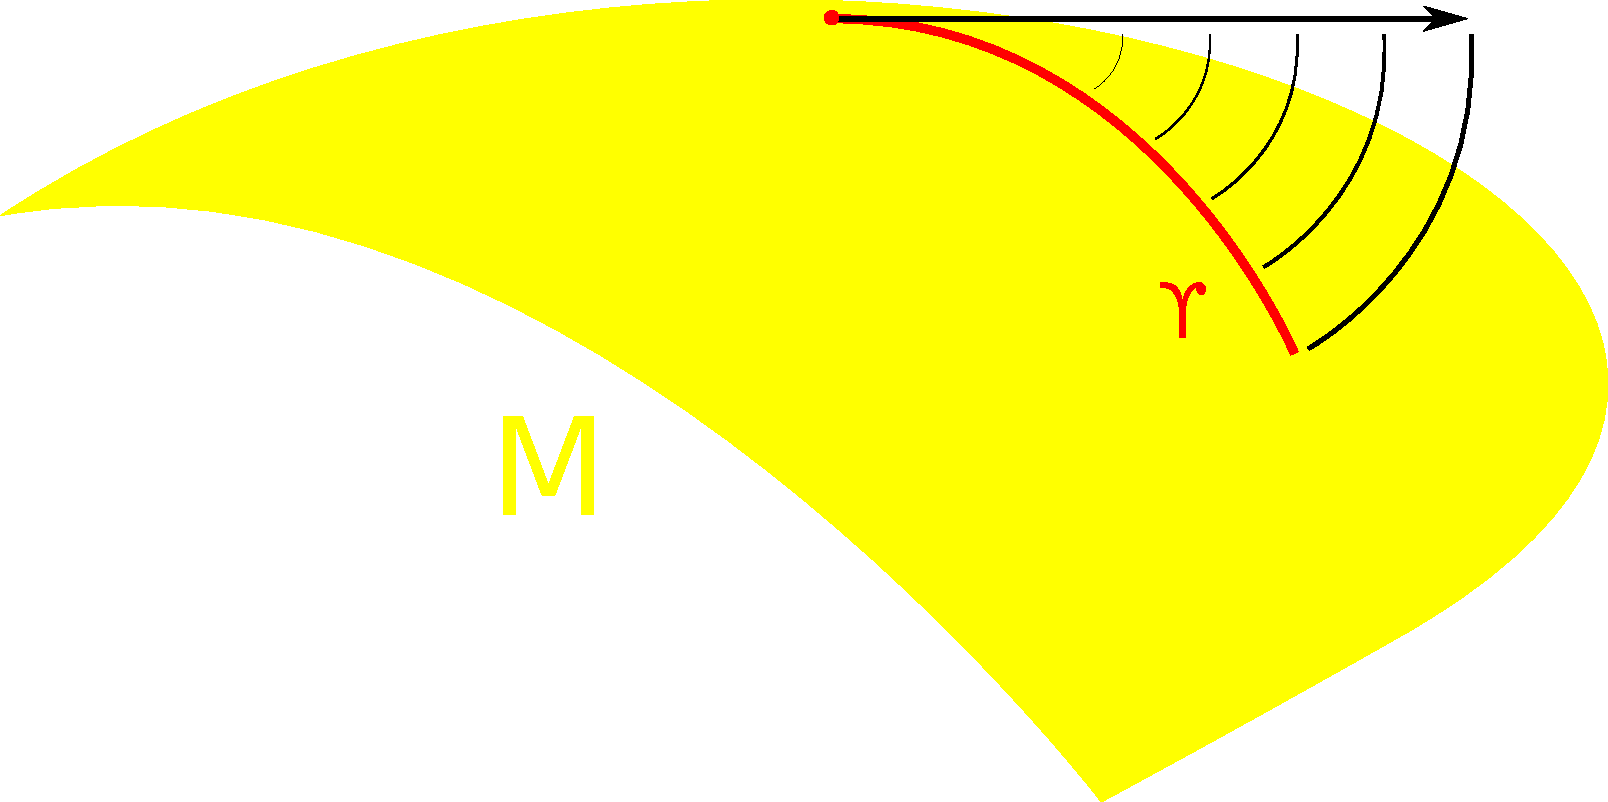
\includegraphics[scale=0.3]{fibrado_tang.pdf}
    \caption{Homotopy equivalence between a geodesic $\gamma\in M^{I}$ and its tangent vector at $\gamma(0)$.}
    \end{figure}

    Thus, Proposition \ref{fht_tang} allows us to state that the notion of tangent bundle can be extended from the concept of smooth 
    manifolds to topological manifolds.

    \begin{prop}\label{iso_homeo}
    If $h:M\to N$ is a homeomorphism between topological manifolds, then $(\tau M,\tau_{0}M)\sim_{f}h^{*}(\tau N,\tau_{0}N)$.
    \end{prop}

    \begin{proof}
        
    \

    Since $h$ is a homeomorphism, the map $H:(TM,T_{0}M)\to (TN,T_{0}N)$ given by $H(\omega)=h\circ\omega$ is one ass well, with inverse 
    $H^{-1}(\omega)=h^{-1}\circ\omega$.

    If we denote by $p:TM\to M$ and $q:TN\to N$ the projections of $(\tau M,\tau_{0}M)$ and $(\tau N,\tau_{0}N)$, respectively, then the 
    map $h^{-1}\circ q\circ H:TM\to M$ satisfies $h^{-1}\circ q\circ H(\omega)=p(\omega)$.

    Thus, Lemma \ref{iso_homot_2} guarantees that $(\tau M,\tau_{0}M)\sim_{f}h^{*}(\tau N,\tau_{0}N)$.

    \end{proof}

    Let us now see that the notion of generalized tangent bundle is natural with respect to the Cartesian product of topological manifolds, 
    in the following sense:

    \begin{prop}\label{fht_tang_cart}
        Let $M$ and $S$ be two arbitrary topological manifolds. Then:
        
        $$ (\tau (M\times S),\tau_{0}(M\times S))\sim_{f} (\tau M,\tau_{0}M)\times (\tau S,\tau_{0}S) $$
    \end{prop}
    \begin{proof}

    \

    Initially, consider $(\tau M,\tau_{0}M)=(TM,T_{0}M,p,M)$, $(\tau S,\tau_{0}S)=(TS,T_{0}S,q,S)$, and 
    $(\tau (M\times S),\tau_{0}(M\times S))=(T(M\times S),T_{0}(M\times S),r,M\times S)$. Denote the product 
    $(\tau M,\tau_{0}M)\times (\tau S,\tau_{0}S)=(E,E_{0},p\times q,M\times S)$, where:
    $$ E=(TM)\times(TS) $$
    $$ E_{0}=[(TM)\times (T_{0}S)]\bigcup [(T_{0}M)\times (TS)] $$

    \

    Consequently, the map $\phi:(T(M\times S),T_{0}(M\times S))\to (E,E_{0})$ defined by $\phi(\omega)=(p_{1}\circ\omega,p_{2}\circ\omega)$ 
    is well defined, because if $\omega\in T_{0}(M\times S)$, then $\omega(t)\neq \omega(0)$ for all $0<t\leq 1$. That is, $p_{i}\circ\omega(t)\neq p_{i}\circ\omega(0)$ for all $0<t\leq 1$ and $i=1$ or $2$, and thus, $p_{i}\circ\omega\in E_{0}$ for $i=1$ or $2$.

    On the other hand, observe that $\phi$ is a homeomorphism whose inverse map $\phi^{-1}:(E,E_{0})\to (T(M\times S),T_{0}(M\times S))$ is 
    naturally given by $\phi^{-1}(\omega_{1},\omega_{2})=(\omega_{1},\omega_{2})$. Moreover, it is clear that $(p\times q)\circ\phi=r$.

    Thus, it follows from Lemma \ref{iso_homot} that:
    $$(\tau (M\times S),\tau_{0}(M\times S))\sim_{f} (\tau M,\tau_{0}M)\times (\tau S,\tau_{0}S)$$

    \end{proof}



    \subsection{Generalized Normal Bundle of a Local-Flat Embedding}\label{secao_fht_normal}

    \

    In this subsection, we will show that the concept of generalized bundle\index{bundle!generalized} also allows the generalization of the 
    notion of normal vector bundle\index{bundle!vector!normal} from smooth manifolds\index{manifold!smooth} to topological 
    manifolds\index{manifold!topological}.

    Before moving forward, we recall\footnote{For more details, see (\cite{lee_s}, Proposition 5.16, p. 106).} that if \( M^{m} \) and 
    \( S^{m+k} \) are smooth manifolds and if \( i:M\hookrightarrow S \) is a smooth embedding\index{embedding!smooth}, then \( i(M) \) 
    constitutes a smooth submanifold of \( S \) such that, for every \( b\in M \), there exists an open neighborhood \( U\subset S \) of 
    \( i(b) \) with \( (U,U\cap i(M))\approx (\mathbb{R}^{m+k},\mathbb{R}^{m}) \).
    
    This feature leads us to the following:
    
    \begin{defi}
        A topological embedding\index{embedding!topological} \( i:M^{m}\hookrightarrow S^{m+k} \), between topological manifolds, is said to 
        be locally-flat, or simply local-flat\index{embedding!local-flat}, if for every \( b\in M \), there exists an open neighborhood 
        \( U\subset S \) of \( i(b) \) such that \( (U,U\cap i(M))\approx (\mathbb{R}^{m+k},\mathbb{R}^{m}) \).
    \end{defi}
    
    In the notation of the definition above, since \( M\approx i(M) \), we can rewrite \( M^{m}\subset S^{m+k} \) as a local-flat embedding 
    such that \( (U,U\cap M)\approx (\mathbb{R}^{m+k},\mathbb{R}^{m}) \). The notation used to describe a local-flat embedding will depend 
    on the problem at hand.

    \
    
    For the next result, consider:
    \begin{itemize}
        \item $M^{m}\subset S^{m+k}$ a local-flat embedding
        \item $N_{0}=\{ \omega\in S^{I} \ : \ \omega(t)\in M \Leftrightarrow t=0 \}$
        \item $N=N_{0}\bigcup \{ \omega\in S^{I} \ : \ \omega(t)=\omega(0)\in M, \ \forall t\in I \}$
        \item $q:N\to M$ given by $q(\omega)=\omega(0)$
    \end{itemize}

    \
    
    Thus:
    
    \begin{prop}
        Let $M^{m}\subset S^{m+k}$ be a local-flat embedding\index{embedding!local-flat}. Then, the pair 
        $(\mathcal{N},\mathcal{N}_{0})=(N,N_{0},q,M)$ is a locally trivial\index{locally trivial} $\R^{k}-$generalized bundle.
    \end{prop}
    
    The proof of the proposition above can be found in (\cite{fadell_1}, Proposition 4.1, p. 496).
    
    \begin{defi}
        We call $(\mathcal{N},\mathcal{N}_{0})$ the $\R^{k}-$generalized normal bundle\index{bundle!generalized!normal} of the local-flat 
        embedding $M^{m}\subset S^{m+k}$.
    \end{defi}
    
    On the other hand, consider $M^{m}\subset\R^{m+k}$ a smooth embedding\index{embedding!smooth} of a smooth manifold\index{manifold!smooth} 
    into Euclidean space, and let $\eta$ be the normal $\R^{k}$-vector bundle\index{bundle!vector!normal} of this embedding, as in 
    Definition \ref{defi_fvn}. Thus, we have the following relation between the normal vector bundle and the generalized normal bundle of the 
    local-flat embedding $M\subset \R^{m+k}$:
    
    \begin{prop}
        $(\eta,\eta_{0})\sim_{f} (\mathcal{N},\mathcal{N}_{0})$
    \end{prop}
    
    The proof of the proposition above can be found in (\cite{fadell_1}, Corollary 4.9, p. 498).
    
    In (\cite{fadell_1}, Theorem 4.11, p. 498), Fadell shows that Theorem \ref{dualidade_whitney_vet} is valid in the context of local-flat 
    embeddings, as follows:
    
    \begin{teo}\label{iso_merg_lf_1}
        If $M^{m}\subset S^{m+k}$ is a local-flat embedding with $\R^{k}-$generalized normal bundle $(\mathcal{N},\mathcal{N}_{0})$, then:
        $$ (\tau M,\tau_{0}M)\oplus (\mathcal{N},\mathcal{N}_{0})\sim_{f} (\tau S,\tau_{0}S)_{|M} $$
    \end{teo}
    
    Furthermore, we can obtain the following:

    \begin{prop}\label{iso_merg_lf_2}
        If $i:M^{m}\hookrightarrow S^{m+k}$ is a local-flat embedding\index{embedding!local-flat}, then:
        $$ (\tau S,\tau_{0}S)_{|M}\sim_{f} i^{*}(\tau S,\tau_{0}S) $$
    \end{prop}
    \begin{proof}

        \
        
        First, let us fix the following notations:
        
        \begin{enumerate}
            \item $(\tau S,\tau_{0}S)=(T,T_{0},p,S)$, where:
            \begin{itemize}
                \item $T_{0}=\{ \omega\in S^{I} \ : \ \omega(t)=\omega(0) \Leftrightarrow t=0 \}$
                \item $T=T_{0}\bigcup \{ \omega\in S^{I} \ : \ \omega(t)=\omega(0), \ \forall t\in I \}$
                \item $p:T\to S$ given by $p(\omega)=\omega(0)$
            \end{itemize}
            \item $(\tau S,\tau_{0}S)_{|M}=(p^{-1}(M),p^{-1}(M)\cap T_{0},q,M)$, where:
            \begin{itemize}
                \item $p^{-1}(M)=\{ \omega\in T \ : \ \omega(0)\in M \}$
                \item $p^{-1}(M)\cap T_{0}=\{ \omega\in T_{0} \ : \ \omega(0)\in M \}$
                \item $q=p_{|p^{-1}(M)}:p^{-1}(M)\to M$ given by $q(\omega)=\omega(0)$
            \end{itemize}
            \item $i^{*}(\tau S,\tau_{0}S)=(i^{*}T,i^{*}T_{0},p_{1},M)$, where:
            \begin{itemize}
                \item $i^{*}T=\{ (b,\omega)\in M\times T \ : \ i(b)=\omega(0) \}$
                \item $i^{*}T_{0}=\{ (b,\omega)\in i^{*}T \ : \ \omega\in T_{0} \}$
                \item $p_{1}:i^{*}T\to M$ given by $p_{1}(b,\omega)=b$
            \end{itemize}
        \end{enumerate}
        
        Thus, the fiber map $\phi:(p^{-1}(M),p^{-1}(M)\cap T_{0})\to (i^{*}T,i^{*}T_{0})$ given by $\phi(\omega)=(\omega(0),\omega)$ is 
        well-defined.

        On the other hand, note that the map $\psi:(i^{*}T,i^{*}T_{0})\to (p^{-1}(M),p^{-1}(M)\cap T_{0})$ given by $\psi(b,\omega)=\omega$ is 
        also well-defined.
        
        Furthermore, it is clear that $\phi$ is a homeomorphism with inverse $\psi$. Thus, Lemma \ref{iso_homot} guarantees that 
        $(\tau S,\tau_{0}S)_{|M}\sim_{f} i^{*}(\tau S,\tau_{0}S)$.
        
    \end{proof}

    \
    
    With this, we conclude in this chapter the study of generalized bundles\index{bundle!generalized}, a concept developed by Fadell in \cite{fadell_1} to generalize the notions of tangent\index{bundle!vector!tangent} and normal\index{bundle!vector!normal} vector bundles from the context of smooth manifolds\index{manifold!smooth} to topological manifolds\index{manifold!topological}, where we presented here only the intuitive proof, based on Nash's ideas in \cite{nash}, of how the generalization of the tangent vector bundle occurs.
    
    In order to not only present a modern reinterpretation of the first half of the results presented by Fadell in \cite{fadell_1}, but also to complement \cite{fadell_1}, we have carefully shown in detail how the generalized bundles indeed generalize vector bundles\index{bundle!vector}, as well as how the notion of vector bundle isomorphism is preserved when extended to the category of generalized bundles.
    
    It is worth noting that we also developed in this chapter the concept of pullback generalized bundle\index{bundle!generalized!pullback}, as well as some consequences of such a bundle, a concept that was not mentioned by Fadell in \cite{fadell_1}.
    
    In any case, the results about generalized bundles carefully developed in this chapter suggest that we view this concept as a theory in itself and not just as a tool to construct characteristic classes, as we will present in the following chapter.
    




    \chapter{Characteristic Classes of Topological Manifolds}\label{cap_clas_carac}
    \thispagestyle{empty}
    
    \
    
    In this chapter, we will construct the Thom\index{class!Thom} classes, Stiefel-Whitney\index{class!Stiefel-Whitney} classes, and 
    Euler\index{class!Euler} classes of generalized bundles\index{bundle!generalized}, and present some consequences of such objects. 
    In particular, we will examine the behavior of these classes for the generalized tangent bundles\index{bundle!generalized!tangent} of 
    topological manifolds\index{manifold!topological}.
    
    To that end, in Section \ref{secao_thom}, we will introduce the concept of orientability of generalized bundles, which was originally 
    proposed by Fadell in \cite{fadell_1}, in order to guarantee the existence of the Thom class and Thom isomorphism for such bundles. 
    We will also discuss how the Thom class behaves in specific generalized bundles.
    
    In Section \ref{secao_SW}, we will define the Stiefel-Whitney classes of generalized bundles in a manner identical to the definition of 
    the Stiefel-Whitney classes of vector bundles\index{bundle!vector} presented in \cite{milnor_1}. Furthermore, we will see how the notion 
    of pullback generalized bundle introduced in the previous chapter will be relevant to deduce some consequences concerning the 
    Stiefel-Whitney classes, since Fadell did not address this concept in \cite{fadell_1}.
    
    Concluding the chapter, in Section \ref{secao_euler}, we will define the Euler class of generalized bundles, a topic that was scarcely 
    addressed by Fadell in \cite{fadell_1}. In this section, we will present several well-known results about Euler classes of vector 
    bundles and smooth manifolds, but in their versions for generalized bundles and topological manifolds.
    
    As explained in Remark \ref{obs_varied_bordo}, we emphasize that every topological manifold mentioned in this chapter will be a 
    manifold without boundary.
    


    \section{Orientability and Thom Class}\label{secao_thom}

    \

    Before constructing the Stiefel–Whitney\index{class!Stiefel–Whitney} and Euler\index{class!Euler} classes of generalized 
    bundles\index{bundle!generalized}, we need to introduce the concept of orientability of these bundles. This concept will be fundamental 
    to ensure the existence of the Thom class\index{class!Thom} and the Thom isomorphism\index{isomorphism!Thom}, as will be seen later.

    The concept of orientability of generalized bundles was proposed by Fadell in \cite{fadell_1}. However, Fadell did not delve deeply into 
    this matter, since the main topic developed in \cite{fadell_1} concerned the Stiefel–Whitney classes, for which there is no need to 
    address orientability.

    In this section, we will explore in more detail the notion of orientability of generalized bundles and present some technical results 
    about the Thom class—more specifically, the behavior of the Thom class in pullback\index{bundle!generalized!pullback} and 
    product\index{bundle!generalized!product} generalized bundles, what happens when we reverse the orientation of a generalized bundle, and 
    the relationship between the dimension of a topological manifold and the Thom class of its tangent generalized 
    bundle\index{bundle!generalized!tangent}.

    With the exception of Lemmas \ref{lema_thom_2}, \ref{lema_thom_3}, \ref{lema_thom_4}, and \ref{lema_thom_5}, the results presented in 
    this section were taken from \cite{fadell_1}.

    Thus, let us first consider $(\mathcal{F},\mathcal{F}_{0})=(E,E_{0},p,B)$ to be a $\R^{n}-$ generalized bundle\index{bundle!generalized}, 
    and the following set:
    $$ \Omega_{p}=\{ (e,\omega)\in E\times B^{I} \ : \ p(e)=\omega(0) \} $$

    \

    In particular, since $(\mathcal{F},\mathcal{F}_{0})$ is a pair fibration\index{fibration!pair}, then by defining the maps 
    $h:\Omega_{p}\to E$ and $H:\Omega_{p}\times I\to B$ by $h(e,\omega)=e$ and $H((e,\omega),t)=\omega(t)$, respectively, there exists a 
    map $\wt{H}:\Omega_{p}\times I\to E$ such that the following diagram commutes:

    $$ \xymatrix @C=0.5cm {
    	\Omega_{p}\times \{0\}\ar[rrrrr]^-{h} \ar@{^(->}[ddd] &&&&& E \ar[ddd]^-{p} \\
    	&&&&& \\		 
    	&&&&& \\				 
    	\Omega_{p}\times I \ar[rrrrr]^-{H} \ar[rrrrruuu]^-{\wt{H}} &&&&& B
    } $$

    \

    Moreover, if $(e,\omega)\in \Omega_{p}$ is such that $h(e,\omega)\in E_{0}$, then $\wt{H}((e,\omega),\_) \in E_{0}$. 
    In this way, we can define the map $\lambda:\Omega_{p}\to E^{I}$ by $\left[ \lambda(e,\omega) \right](t)=\wt{H}((e,\omega),t)$.

    Thus, fixing the fiber $(F,F_{0})$ of $(\mathcal{F},\mathcal{F}_{0})$ over $b_{0}\in B$, the following map is well-defined:
    $$ \Omega(B,b_{0})\times (F,F_{0}) \to (F,F_{0}) $$
    $$ (\omega,e)\longmapsto \omega\cdot e=\left[ \lambda(e,\omega) \right](1)  $$

    \

    Note that, fixing $\omega\in \Omega(B,b_{0})$, it is evident that the map $(F,F_{0})\to (F,F_{0})$, which sends $e\mapsto \omega\cdot e$, 
    induces an action of $\Omega(B,b_{0})$ on $H_{n}(F,F_{0};R)$ for any commutative unital ring $R$.

    With this, we have the following:

    \begin{defi}{\bf (Orientability)}\label{defi_orient}
    	A $\R^{n}-$ generalized bundle $(\mathcal{F},\mathcal{F}_{0})$ over $B$ is said to be 
        $R-$orientable\index{bundle!generalized!orientable} if, for every $b_{0}\in B$, the action of $\Omega(B,b_{0})$ on $H_{n}(F,F_{0};R)$ 
        defined above is trivial, where $(F,F_{0})$ denotes the fiber of $(\mathcal{F},\mathcal{F}_{0})$ over $b_{0}\in B$.
    \end{defi}

    Naturally, the orientation of a topological manifold\index{manifold!topological} is directly related to the orientation of its tangent 
    generalized bundle\index{bundle!generalized!tangent}, as we state in the next result, whose proof can be found in 
    (\cite{fadell_1}, Proposition 3.16, p. 495).

    \begin{prop}\label{propriedade_orient_var}
    	A topological manifold $M$ is $R-$orientable if and only if its generalized tangent bundle $(\tau M,\tau_{0}M)$ is $R$-orientable.
    \end{prop}

    \begin{obs}
    	Every generalized bundle is $\Z_{2}-$orientable, as guaranteed in (\cite{allaud}, Corollary 2.8, p. 243).
    \end{obs}

    With the aim of defining the Stiefel–Whitney\index{class!Stiefel–Whitney} classes of any generalized bundle and the 
    Euler\index{class!Euler} class of a $\Z-$orientable generalized bundle, we need to ensure the existence of the Thom class and Thom 
    isomorphism, just as it is done for vector bundles\index{bundle!vector}, as in (\cite{milnor_1}, Chapters 8, 9, and 10).

    \begin{teo}\label{teo_iso_thom_fht}
    	Let $(\mathcal{F},\mathcal{F}_{0})=(E,E_{0},p,B)$ be an $R-$orientable $\R^{n}-$ generalized bundle. Then, there exists a unique class 
        $\tau\in H^{n}(E,E_{0};R)$ such that the homomorphism $\phi:H^{k}(B;R)\to H^{n+k}(E,E_{0};R)$, given by $\phi(x)=p^{*}(x)\ccup \tau$, 
        is an isomorphism for every integer $k\geq 0$. Moreover, letting $i:(F,F_{0})\hookrightarrow (E,E_{0})$ be the inclusion of a fiber 
        $(F,F_{0})$ of $(\mathcal{F},\mathcal{F}_{0})$ into its total space, and $(u)=H^{n}(F,F_{0};R)\cong R$, the class $\tau$ is uniquely 
        determined by $i^{*}(\tau)=u$.
    \end{teo}

    The proof of the theorem above can be found in (\cite{fadell_1}, Theorem 5.2, p. 502).

    \begin{obs}\label{obs_proj_iso}
    	In the course of the proof of Theorem \ref{teo_iso_thom_fht}, it is shown that the induced maps 
        $i^{*}:H^{n}(E,E_{0};R)\to H^{n}(F,F_{0};R)$ and $p^{*}:H^{k}(B;R)\to H^{k}(E;R)$ are isomorphisms for all $k\geq 0$.
    \end{obs}

    \begin{defi}{\bf (Thom Class and Thom Isomorphism)}\label{defi_thom}
    	Given an $R-$orientable $\R^{n}-$ generalized bundle $(\mathcal{F},\mathcal{F}_{0})=(E,E_{0},p,B)$, the generator 
        $(\tau)=H^{n}(E,E_{0};R)\cong R$ is called the Thom class\index{class!Thom}, and the isomorphism 
        $\phi:H^{k}(B;R)\to H^{n+k}(E,E_{0};R)$ from Theorem \ref{teo_iso_thom_fht} is referred to as the Thom 
        isomorphism\index{isomorphism!Thom} of $(\mathcal{F},\mathcal{F}_{0})$.
    \end{defi}

    Now, let us examine some consequences involving orientability and the Thom classes of generalized bundles. Since we will be working with 
    Stiefel–Whitney\index{class!Stiefel–Whitney} and Euler\index{class!Euler} classes throughout this chapter, the final lemmas of this 
    section will be stated for $R=\Z_{2}$ and $R=\Z$.

    %\begin{lem}\label{lema_thom_1}
    %Let $(\mathcal{F},\mathcal{F}_{0})$ and $(\mathcal{F'},\mathcal{F'}_{0})$ be two generalized $\R^{n}$-bundles over the same base such that $(\mathcal{F},\mathcal{F}_{0})\sim_{f}(\mathcal{F'},\mathcal{F'}_{0})$. Then:
    %	\begin{enumerate}
    %		\item $(\mathcal{F},\mathcal{F}_{0})$ is $R$-orientable if and only if $(\mathcal{F'},\mathcal{F'}_{0})$ is $R$-orientable;
    %		\item if $(\mathcal{F},\mathcal{F}_{0})$ is $R$-orientable\index{bundle!generalized!orientable} and we denote by $\tau$ and $\tau'$ the Thom classes\index{class!Thom} of $(\mathcal{F},\mathcal{F}_{0})$ and $(\mathcal{F'},\mathcal{F'}_{0})$, respectively, then the fiber map $f:(\mathcal{F},\mathcal{F}_{0})\to (\mathcal{F'},\mathcal{F'}_{0})$ guaranteed by Definition \ref{defi_iso_homot} is such that $f^{*}(\tau')=\tau$.
    %	\end{enumerate}
    %\end{lem}
    %\begin{proof}
    %
    %\
    %
    %\ A
    %
    %\end{proof}

    \begin{lem}\label{lema_thom_2}
    	Let $(\mathcal{F},\mathcal{F}_{0})$ be an $R-$orientable\index{bundle!generalized!orientable} $\R^{n}-$ generalized bundle over a 
        base $B$, let $f:B'\to B$ be any map, and let $\tau$ be the Thom class\index{class!Thom} of $(\mathcal{F},\mathcal{F}_{0})$. Then:
    	\begin{enumerate}
    		\item $f^{*}(\mathcal{F},\mathcal{F}_{0})$ is an $R-$orientable $\R^{n}-$ generalized bundle.
    		\item If $\tau^{*}$ is the Thom class of $f^{*}(\mathcal{F},\mathcal{F}_{0})$, then $\tau^{*}=1\times \tau$.
    	\end{enumerate}
    \end{lem}
    \begin{proof}

        \

        First, denoting $(\mathcal{F},\mathcal{F}_{0})=(E,E_{0},p,B)$, we already know from Lemma \ref{fht_pullback} that 
        $f^{*}(\mathcal{F},\mathcal{F}_{0})=(f^{*}E,f^{*}E_{0},p_{1},B')$ is a generalized $\R^{n}-$bundle, where:
        $$f^{*}E=\{ (b',e)\in B'\times E \ : \ f(b')=p(e) \}$$
        $$f^{*}E_{0}=\{ (b',e)\in f^{*}E \ : \ e\in E_{0} \}$$

        \

        Now, fixing $b'_{0}\in B'$ and $f(b'_{0})\in B$, let $(F^{*},F^{*}_{0})$ and $(F,F_{0})$ be the fibers of 
        $f^{*}(\mathcal{F},\mathcal{F}_{0})$ and $(\mathcal{F},\mathcal{F}_{0})$ over $b'_{0}\in B'$ and $f(b'_{0})\in B$, respectively. 
        Due to Lemma \ref{pf_pullback}, we also know that $(F^{*},F^{*}_{0})=\{ b'_{0} \}\times (F,F_{0})$.

        Thus, the action defined in Definition \ref{defi_orient} of $\Omega(B',b'_{0})$ on $H_{n}(F^{*},F^{*}_{0};R)$ reduces to the 
        action of $\Omega(B,f(b'_{0}))$ on $H_{n}(F,F_{0};R)$.

        Since $(\mathcal{F},\mathcal{F}_{0})$ is an $R-$orientable generalized bundle, the action of $\Omega(B,f(b'_{0}))$ on 
        $H_{n}(F,F_{0};R)$ is trivial. Therefore, the action of $\Omega(B',b'_{0})$ on $H_{n}(F^{*},F^{*}_{0};R)$ is also trivial, and 
        consequently, $f^{*}(\mathcal{F},\mathcal{F}_{0})$ is an $R-$orientable generalized bundle.

        \

        Finally, denoting the Thom classes\index{Thom!class} of $(\mathcal{F},\mathcal{F}_{0})$ and $f^{*}(\mathcal{F},\mathcal{F}_{0})$ 
        respectively by the generators $(\tau)=H^{n}(E,E_{0};R)$ and $(\tau^{*})=H^{n}(f^{*}E,f^{*}E_{0};R)$, we will prove that 
        $\tau^{*}=1\times\tau$.

        To do so, consider $i:(F,F_{0})\hookrightarrow (E,E_{0})$ and $j:(F^{*},F^{*}_{0})\hookrightarrow (f^{*}E,f^{*}E_{0})$ the canonical 
        inclusions. Since $(F^{*},F^{*}_{0})=\{ b'_{0} \}\times (F,F_{0})$, it follows that $j=1\times i$.

        Now, fixing the generators $(u)=H^{n}(F,F_{0};R)$ and 
        $(1\times u)=H^{n}(F^{*},F^{*}_{0};R)$\footnote{The Künneth formula\index{Künneth!formula} allows us to assert that 
        $1\times u$ is a generator of $H^{n}(F^{*},F^{*}_{0};R)$.}, recall that the Thom classes $\tau$ and $\tau^{*}$ are uniquely 
        determined so that $i^{*}(\tau)=u$ and $j^{*}(\tau^{*})=1\times u$.

        However, note that:

        \

        $\begin{array}{rl}
        	j^{*}(1\times \tau) \ = & (1\times i)^{*}(1\times \tau) \\
        	= & 1\times i^{*}(\tau) \\
        	= & 1\times u
        \end{array}$

        \

        Therefore, by uniqueness, we conclude that $\tau^{*}=1\times \tau$.

    \end{proof}

    \begin{lem}\label{lema_thom_3}
	    Let $(\mathcal{F},\mathcal{F}_{0})$ be an $\R^{n}-$generalized bundle\index{generalized bundle!orientable}, 
        $(\mathcal{F'},\mathcal{F'}_{0})$ an $\R^{m}-$generalized bundle, both $R-$orientable. Denoting by $\tau$ and $\tau'$ 
        the Thom classes\index{Thom class} of $(\mathcal{F},\mathcal{F}_{0})$ and $(\mathcal{F'},\mathcal{F'}_{0})$, respectively, then:
	\begin{enumerate}
		\item $(\mathcal{F},\mathcal{F}_{0})\times (\mathcal{F'},\mathcal{F'}_{0})$ is an $\R^{n+m}-$generalized $R-$orientable bundle.
		\item If $\tau''$ is the Thom class of $(\mathcal{F},\mathcal{F}_{0})\times (\mathcal{F'},\mathcal{F'}_{0})$, 
        then $\tau''=\tau\times\tau'$.
	\end{enumerate}
    \end{lem}

    \begin{proof}

        \

    	Recalling Lemma \ref{fht_produto}, we know that $(\mathcal{F},\mathcal{F}_{0})\times (\mathcal{F'},\mathcal{F'}_{0})$ is an 
        $\R^{n+m}-$generalized bundle. Furthermore, we denote $(\mathcal{F},\mathcal{F}_{0})=(E,E_{0},p,B)$, 
        $(\mathcal{F'},\mathcal{F'}_{0})=(E',E'_{0},q,B')$, and 
        $(\mathcal{F},\mathcal{F}_{0})\times (\mathcal{F'},\mathcal{F'}_{0})=(E'',E''_{0},r,B'')$, where:

        \

    	$E''=E\times E'$

    	$E''_{0}=\left( E\times E'_{0} \right)\cup \left( E_{0}\times E' \right)$
        
    	$r=p\times q$

    	$B''=B\times B'$

        \

    	Let $b_{0}\in B$, $b'_{0}\in B'$, and $(b_{0},b'_{0})\in B''$. Consider $(F,F_{0})$, $(F',F'_{0})$, and $(F'',F''_{0})$ as the fibers 
        of $(\mathcal{F},\mathcal{F}_{0})$, $(\mathcal{F'},\mathcal{F'}_{0})$, and 
        $(\mathcal{F},\mathcal{F}_{0})\times (\mathcal{F'},\mathcal{F'}_{0})$ over $b_{0}\in B$, $b'_{0}\in B'$, and $(b_{0},b'_{0})\in B''$, 
        respectively.

    	Since $(F'',F''_{0})=(F,F_{0})\times (F',F'_{0})$, the Künneth formula\index{Künneth formula} guarantees us that:
    	$$ H_{n+m}(F'',F''_{0};R)\cong H_{n}(F,F_{0};R)\tensor H_{m}(F',F'_{0};R) $$

    	Moreover, we also have the following homeomorphism:
    	$$ \Omega(B'',(b_{0},b'_{0}))\approx \Omega(B,b_{0})\times\Omega(B',b'_{0}) $$

        \

    	Therefore, the action given in Definition \ref{defi_orient} of $\Omega(B'',(b_{0},b'_{0}))$ on $H_{n+m}(F'',F''_{0};R)$ reduces to the 
        actions of $\Omega(B,b_{0})$ and $\Omega(B',b'_{0})$ on $H_{n}(F,F_{0};R)$ and $H_{m}(F',F'_{0};R)$, respectively.

    	Since $(\mathcal{F},\mathcal{F}_{0})$ and $(\mathcal{F'},\mathcal{F'}_{0})$ are $R-$orientable generalized bundles, the actions of 
        $\Omega(B,b_{0})$ and $\Omega(B',b'_{0})$ on $H_{n}(F,F_{0};R)$ and $H_{m}(F',F'_{0};R)$, respectively, are trivial. Thus, the action 
        of $\Omega(B'',(b_{0},b'_{0}))$ on $H_{n+m}(F'',F''_{0};R)$ is trivial and, consequently, 
        $(\mathcal{F},\mathcal{F}_{0})\times (\mathcal{F'},\mathcal{F'}_{0})$ is an $R-$orientable generalized bundle.

        \

    	Finally, let $(\tau)=H^{n}(E,E_{0};R)$, $(\tau')=H^{m}(E',E'_{0};R)$, and $(\tau'')=H^{n+m}(E'',E''_{0};R)$ be the Thom classes of 
        $(\mathcal{F},\mathcal{F}_{0})$, $(\mathcal{F'},\mathcal{F'}_{0})$, and 
        $(\mathcal{F},\mathcal{F}_{0})\times (\mathcal{F'},\mathcal{F'}_{0})$, respectively. We now prove that $\tau''=\tau\times\tau'$.

    	Consider the canonical inclusions $i:(F,F_{0})\hookrightarrow (E,E_{0})$, $i':(F',F'_{0})\hookrightarrow (E',E'_{0})$, and 
        $i'':(F'',F''_{0})\hookrightarrow (E'',E''_{0})$. Since $(F'',F''_{0})=(F,F_{0})\times (F',F'_{0})$ and 
        $(E'',E''_{0})=(E,E_{0})\times (E',E'_{0})$, then $i''=i\times i'$.

    	Fix the generators $(u)=H^{n}(F,F_{0};R)$, $(u')=H^{m}(F',F'_{0};R)$, and 
        $(u\times u')=H^{n+m}(F'',F''_{0};R)$\footnote{The Künneth formula\index{Künneth formula} guarantees that $u\times u'$ is a generator 
        of $H^{n+m}(F'',F''_{0};R)$.} and recall that the Thom classes $\tau$, $\tau'$, and $\tau''$ are uniquely characterized by the 
        equalities $i^{*}(\tau)=u$, $i'^{*}(\tau')=u'$, and $i''^{*}(\tau'')=u\times u'$, respectively.

    	However, note that:

        \
    	
    	$\begin{array}{rl}
    		i''^{*}(\tau\times\tau') \ = & (i\times i')^{*}(\tau\times\tau') \\
    		= & i^{*}(\tau)\times i'^{*}(\tau') \\
    		= & u\times u'
    	\end{array}$

        \

    	Hence, by uniqueness, we conclude that $\tau''=\tau\times\tau'$.

    \end{proof}

    \begin{lem}\label{lema_thom_4}
    Let $(\mathcal{F},\mathcal{F}_{0})$ be a $\R^{n}-$generalized bundle\index{bundle!generalized!orientable} that is $\Z-$orientable, and 
    let $\tau$ be its Thom class\index{class!Thom}. Denoting by $-(\mathcal{F},\mathcal{F}_{0})$ the same $\R^{n}-$generalized bundle with 
    the orientation reversed, and by $\tau'$ its Thom class, then $\tau'=-\tau$.
    \end{lem}

    \begin{proof}

        \

        Let us denote by $(E,E_{0})$ the total space of $(\mathcal{F},\mathcal{F}_{0})$ and by $(F,F_{0})$ an arbitrary fiber of $(\mathcal{F},\mathcal{F}_{0})$.

        The result follows directly from Theorem \ref{teo_iso_thom_fht} and Definition \ref{defi_thom}, since the Thom class of $(\mathcal{F},\mathcal{F}_{0})$ is the generator $(\tau)=H^{n}(E,E_{0};\Z)\cong\Z$, which is directly related to the generator $(u)=H^{n}(F,F_{0};\Z)\cong\Z$, and consequently, the Thom class of $-(\mathcal{F},\mathcal{F}_{0})$ is the generator $(-\tau)=H^{n}(E,E_{0};\Z)\cong\Z$, directly related to the generator $(-u)=H^{n}(F,F_{0};\Z)\cong\Z$.

    \end{proof}

    \begin{lem}\label{lema_thom_5}
        Let $M^{m}$ be a closed topological manifold\index{manifold!topological} that is $\Z-$orientable and of odd dimension, and let 
        $(\tau M,\tau_{0}M)$ be its $\R^{m}-$generalized tangent bundle\index{bundle!generalized!tangent}. Then the Thom 
        class\index{class!Thom} $\tau$ of $(\tau M,\tau_{0}M)$ satisfies $\tau\ccup\tau=0$.
    \end{lem}

    \begin{proof}

        \

        First, since $M^{m}$ is a $\Z-$orientable topological manifold, Proposition \ref{propriedade_orient_var} ensures that the 
        $\R^{m}-$generalized tangent bundle $(\tau M,\tau_{0}M)$ of $M$ is also $\Z-$orientable.

        On the other hand, denoting by $(TM,T_{0}M)$ the total space of $(\tau M,\tau_{0}M)$ and recalling that $M$ is compact, the Thom 
        isomorphism for $(\tau M,\tau_{0}M)$ gives:
        $$ H^{2m}(TM,T_{0}M;\Z)\cong H^{m}(M;\Z)\cong\Z $$

        \

        Therefore, denoting the generator $(\tau)=H^{m}(TM,T_{0}M;\Z)$ as the Thom class of $(\tau M,\tau_{0}M)$, and since item 5 of 
        Lemma \ref{propriedades_produtos} states that $\tau\ccup\tau =(-1)^{m^{2}}(\tau\ccup\tau)$ and $m$ is odd, it follows that 
        $\tau\ccup\tau=-(\tau\ccup\tau)$, i.e., $2(\tau\ccup\tau)=0$.

        Since $2(\tau\ccup\tau)\in H^{2m}(TM,T_{0}M;\Z)\cong\Z$, we conclude that $\tau\ccup\tau=0$.

    \end{proof}



    \section{Stiefel-Whitney Classes}\label{secao_SW}

    \

    The construction of the Stiefel–Whitney classes for generalized bundles\index{bundle!generalized} will follow, due to Theorem 
    \ref{teo_iso_thom_fht}, in exactly the same way as the construction given in (\cite{milnor_1}, Chapter 8) for vector 
    bundles\index{bundle!vector}. Note that, since every generalized bundle is $\Z_{2}-$orientable and the Stiefel–Whitney classes are 
    defined in the context of singular cohomology $\Z_{2}-$modules, we do not need to impose any orientability condition on the generalized 
    bundles throughout this section.

    With the exception of Propositions \ref{res_SW_fht_8} and \ref{res_SW_fht_9}, the results in this section were taken from 
    \cite{fadell_1} and \cite{fadell_4}. Furthermore, it is worth noting that Theorems \ref{res_SW_fht_2} and \ref{res_SW_fht_10}, and 
    Corollary \ref{res_SW_fht_6}, can be found in (\cite{fadell_4}, Lemma 2.11, p. 39), (\cite{fadell_4}, Theorem 5.2, p. 52), and 
    (\cite{fadell_1}, Theorem 6.11, p. 504), respectively. In these references, Fadell presents more technical proofs without using pullback 
    generalized bundles. In contrast, the proofs provided here highlight the importance of the pullback generalized 
    bundle\index{bundle!generalized!pullback}.

    Thus, let $(\mathcal{F},\mathcal{F}_{0})=(E,E_{0},p,B)$ be an $\R^{n}-$generalized bundle and $\phi$ its Thom isomorphism. Then, for 
    every $k\geq 0$, the following composition makes sense:\footnote{$Sq^{k}$ denotes the Steenrod square operation\index{Steenrod square}, 
    some of whose properties can be found in Section \ref{ap_steenrod}.}
    $$ \xymatrix @C=0.5cm {
    	H^{n}(E,E_{0};\Z_{2}) \ar[rrr]^-{Sq^{k}} &&& H^{n+k}(E,E_{0};\Z_{2}) \ar[rrr]^-{\phi^{-1}} &&& H^{k}(B;\Z_{2})
    } $$

    \

    \begin{defi}{\bf (Stiefel–Whitney Classes)}
    	Let $(\mathcal{F},\mathcal{F}_{0})$ be an $\R^{n}-$generalized bundle over a base $B$, and let $\phi$ and $\tau$ denote its Thom 
        isomorphism and Thom class, respectively. For each $k\geq 0$, the $k$th Stiefel–Whitney class\index{class!Stiefel–Whitney} of 
        $(\mathcal{F},\mathcal{F}_{0})$ is defined as:
    	$$ w_{k}(\mathcal{F},\mathcal{F}_{0}) = \phi^{-1} \circ Sq^{k}(u) \in H^{k}(B;\Z_{2}) $$

        \
    
    	We also define the element $W(\mathcal{F},\mathcal{F}_{0}) = \ds\sum_{k\geq 0} w_{k}(\mathcal{F},\mathcal{F}_{0}) \in H^{*}(B;\Z_{2})$ 
        as the total Stiefel–Whitney class\index{class!total Stiefel–Whitney} of $(\mathcal{F},\mathcal{F}_{0})$.
    \end{defi}

    Now, let us examine some consequences of the Stiefel–Whitney classes.

    \begin{teo}\label{res_SW_fht_1}
	Let $(\mathcal{F},\mathcal{F}_{0})$ be a $\R^{n}-$generalized bundle. Then $w_{0}(\mathcal{F},\mathcal{F}_{0})=1$ and 
    $w_{k}(\mathcal{F},\mathcal{F}_{0})=0$ for $k>n$. In other words, 
    $W(\mathcal{F},\mathcal{F}_{0})=1+\ds\sum_{k=1}^{n}w_{k}(\mathcal{F},\mathcal{F}_{0})$.
    \end{teo}

    \begin{proof}
    
        \

        Consider $(\mathcal{F},\mathcal{F}_{0})=(E,E_{0},p,B)$, $\phi$ its Thom isomorphism, and $\tau\in H^{n}(E,E_{0};\Z_{2})$ its Thom 
        class. Since $\phi(1)=\tau$ and $Sq^{0}=1$, we have:

        \

        $\begin{array}{rl}
        	w_{0}(\mathcal{F},\mathcal{F}_{0}) \ = & \phi^{-1}\circ Sq^{0}(\tau) \\
        	= & \phi^{-1}(\tau) \\
        	= & 1
        \end{array}$

        \

        On the other hand, for $k>n$, we have $Sq^{k}=0$, and thus $w_{k}(\mathcal{F},\mathcal{F}_{0})=0$. Therefore, the total 
        Stiefel-Whitney class of $(\mathcal{F},\mathcal{F}_{0})$ is 
        $W(\mathcal{F},\mathcal{F}_{0})=1+\ds\sum_{k=1}^{n}w_{k}(\mathcal{F},\mathcal{F}_{0})$.

    \end{proof}

    Note that, given a $\R^{n}-$generalized bundle $(\mathcal{F},\mathcal{F}_{0})$ over $B$, since Theorem \ref{res_SW_fht_1} guarantees 
    that $w_{0}(\mathcal{F},\mathcal{F}_{0})=1$, the total Stiefel-Whitney class is an invertible 
    element\footnote{See Theorem \ref{teo_elemento_inversivel}.} in the ring $H^{*}(B;\Z_{2})$, whose inverse element will be denoted by 
    $W^{-1}(\mathcal{F},\mathcal{F}_{0})$.

    \begin{teo}\label{res_SW_fht_2}
    	Let $(\mathcal{F},\mathcal{F}_{0})$ and $(\mathcal{F'},\mathcal{F'}_{0})$ be two $\R^{n}-$generalized bundles over $B$ and $B'$, 
        respectively. If $f:B\to B'$ is a map such that $(\mathcal{F},\mathcal{F}_{0})\sim_{f} f^{*}(\mathcal{F'},\mathcal{F'}_{0})$, then 
        $W(\mathcal{F},\mathcal{F}_{0})=f^{*}(W(\mathcal{F'},\mathcal{F'}_{0}))$.
    \end{teo}
    \begin{proof}

        \

        Initially, consider $(\mathcal{F},\mathcal{F}_{0})=(E,E_{0},p,B)$ and $(\mathcal{F'},\mathcal{F'}_{0})=(E',E'_{0},q,B')$, and recall 
        that $f^{*}(\mathcal{F'},\mathcal{F'}_{0})=(f^{*}E',f^{*}E'_{0},p_{1},B)$ is the $\R^{n}-$ generalizedbundle such that:
        $$f^{*}E'=\{ (b,e')\in B\times E' \ : \ f(b)=q(e') \}$$
        $$f^{*}E'_{0}=\{ (b,e')\in f^{*}E' \ : \ e'\in E'_{0} \}$$

        \

        Since $(\mathcal{F},\mathcal{F}_{0})\sim_{f} f^{*}(\mathcal{F'},\mathcal{F'}_{0})$, Definition \ref{defi_iso_homot} ensures that 
        there exists a fibered map\index{map!fibered} $g:(E,E_{0})\to (f^{*}E',f^{*}E'_{0})$ such that $g$ is, in particular, a homotopy 
        equivalence.

        Thus, considering the Thom classes\index{class!Thom} of $(\mathcal{F},\mathcal{F}_{0})$ and $f^{*}(\mathcal{F'},\mathcal{F'}_{0})$ as 
        the generators $(\tau)=H^{n}(E,E_{0};\Z_{2})$ and $(\tau^{*})=H^{n}(f^{*}E',f^{*}E'_{0};\Z_{2})$, respectively, the fact that $g$ is 
        a homotopy equivalence allows us to assert that:
        $$ g^{*}(\tau^{*})=\tau $$

        \

        Conversely, by regarding the Thom class of $(\mathcal{F'},\mathcal{F'}_{0})$ as the generator $(\tau')=H^{n}(E',E'_{0};\Z_{2})$, 
        the canonical projection $p_{2}:(f^{*}E',f^{*}E'_{0})\to (E',E'_{0})$ satisfies, guarantees by Lemma \ref{lema_thom_2}, that :
        $$ p_{2}^{*}(\tau')=\tau^{*}=1\times \tau' $$

        \

        Therefore, we have:
        $$ g^{*}\circ p_{2}^{*}(\tau')=\tau $$

        \

        Furthermore, by definition, we have the following commutative diagram:
        $$ \xymatrix @C=0.5cm {
        	E \ar[rrrrr]^-{g} \ar[rrrrrddd]^-{p} &&&&& f^{*}E' \ar[rrrrr]^-{p_{2}} \ar[ddd]^-{p_{1}} &&&&& E' \ar[ddd]^-{q} \\
        	&&&&& &&&&& \\
        	&&&&& &&&&& \\
        	&&&&& B \ar[rrrrr]^-{f} &&&&& B'
        } $$

        \

        Now, denoting the Thom isomorphisms\index{isomorphism!Thom} of $(\mathcal{F},\mathcal{F}_{0})$ and $(\mathcal{F'},\mathcal{F'}_{0})$ 
        respectively by $\phi:H^{k}(B;\Z_{2})\to H^{k+n}(E,E_{0};\Z_{2})$ and $\phi':H^{k}(B';\Z_{2})\to H^{k+n}(E',E'_{0};\Z_{2})$, we can 
        also assert that $\phi\circ f^{*}=g^{*}\circ p_{2}^{*}\circ\phi'$. Indeed:

        \

        $\begin{array}{rl}
        	\forall x\in H^{*}(B';\Z_{2}), \ g^{*}\circ p_{2}^{*}\circ\phi'(x) \ = & g^{*}\circ p_{2}^{*}(q^{*}(x)\ccup \tau') \\
        	= & [g^{*}\circ p_{2}^{*}\circ q^{*}(x)]\ccup [g^{*}\circ p_{2}^{*}(\tau')] \\
        	= & [p^{*}\circ f^{*}(x)]\ccup \tau \\
        	= & \phi\circ f^{*}(x)
        \end{array}$

        \

        With this, we have:

        \

        $\begin{array}{rl}
        	\forall k\geq 0, f^{*}(w_{k}(\mathcal{F'},\mathcal{F'}_{0})) \ = & f^{*}\circ\phi'^{-1}\circ Sq^{k}(\tau') \\
        	= & \phi^{-1}\circ g^{*}\circ p_{2}^{*}\circ Sq^{k}(\tau') \\
        	= & \phi^{-1}\circ Sq^{k}\circ g^{*}\circ p_{2}^{*}(\tau') \\
        	= & \phi^{-1}\circ Sq^{k}(\tau) \\
        	= & w_{k}(\mathcal{F},\mathcal{F}_{0})
        \end{array}$

        \

        Therefore, $f^{*}(W(\mathcal{F'},\mathcal{F'}_{0}))=W(\mathcal{F},\mathcal{F}_{0})$.

    \end{proof}

    \begin{cor}\label{res_SW_fht 3}
	Let $(\mathcal{F},\mathcal{F}_{0})$ and $(\mathcal{F'},\mathcal{F'}_{0})$ be two $\R^{n}$-generalized bundles over the same base. 
    If $(\mathcal{F},\mathcal{F}_{0})\sim_{f} (\mathcal{F'},\mathcal{F'}_{0})$, then 
    $W(\mathcal{F},\mathcal{F}_{0})=W(\mathcal{F'},\mathcal{F'}_{0})$.
    \end{cor}

    \begin{proof}

        \

    	Let $B$ be the base of both $(\mathcal{F},\mathcal{F}_{0})$ and $(\mathcal{F'},\mathcal{F'}_{0})$, and let $1:B\to B$ be the 
        identity map. From Example \ref{fht_pullback_ex1}, we know that 
        $(\mathcal{F},\mathcal{F}_{0})\sim_{f} 1^{*}(\mathcal{F'},\mathcal{F'}_{0})$.

    	Thus, it follows from Theorem \ref{res_SW_fht_2} that:
    	$$ W(\mathcal{F},\mathcal{F}_{0})=1^{*}(W(\mathcal{F'},\mathcal{F'}_{0}))=W(\mathcal{F'},\mathcal{F'}_{0}) $$

    \end{proof}

    \begin{cor}\label{res_SW_fht_4}
    	If $(\mathcal{F},\mathcal{F}_{0})$ is a trivial $\R^{n}$-generalized bundle\index{generalized bundle!trivial}, then 
        $W(\mathcal{F},\mathcal{F}_{0})=1$.
    \end{cor}

    \begin{proof}

        \

    	Initially, it follows from Theorem \ref{res_SW_fht_1} that $w_{0}(\mathcal{F},\mathcal{F}_{0})=1$.

    	Now, let $B$ be the base of $(\mathcal{F},\mathcal{F}_{0})$. Since $(\mathcal{F},\mathcal{F}_{0})$ is a trivial 
        $\R^{n}$-generalized bundle, we have $(\mathcal{F},\mathcal{F}_{0})\sim_{f} (\varepsilon^{n}_{B},\varepsilon^{n,0}_{B})$. Moreover, 
        given any $b\in B$, let $c:B\to \{ b \}$ be the constant map. From Example \ref{fht_pullback_ex2}, it follows that 
        $(\varepsilon^{n}_{B},\varepsilon^{n,0}_{B})\sim_{f} c^{*}(\varepsilon^{n}_{\{ b \}},\varepsilon^{n,0}_{\{ b \}})$.

    	Thus, combining Corollary \ref{res_SW_fht 3} with Theorem \ref{res_SW_fht_2}, we obtain:
    	$$ W(\mathcal{F},\mathcal{F}_{0})=c^{*}(W(\varepsilon^{n}_{\{ b \}},\varepsilon^{n,0}_{\{ b \}})) $$

        \

    	But since $w_{k}(\varepsilon^{n}_{\{ b \}},\varepsilon^{n,0}_{\{ b \}})\in H^{k}(\{ b \};\Z_{2})=0$ for $k>0$, it follows that 
        $w_{k}(\mathcal{F},\mathcal{F}_{0})=0$ for $k>0$.

    	Therefore, $W(\mathcal{F},\mathcal{F}_{0})=1$.

    \end{proof}

    \begin{teo}\label{res_SW_fht_5}
	Let $(\mathcal{F},\mathcal{F}_{0})$ and $(\mathcal{F'},\mathcal{F'}_{0})$ be an $\R^{n}-$generalized bundle and an $\R^{m}-$generalized 
    bundle, respectively. Then:
	$$ W[(\mathcal{F},\mathcal{F}_{0})\times (\mathcal{F'},\mathcal{F'}_{0})]=W(\mathcal{F},\mathcal{F}_{0})\times W(\mathcal{F'},\mathcal{F'}_{0}) $$
    \end{teo}
    \begin{proof}

        \

    	Initially, let us denote $(\mathcal{F},\mathcal{F}_{0})=(E,E_{0},p,B)$, $(\mathcal{F'},\mathcal{F'}_{0})=(E',E'_{0},q,B')$ and recall 
        that $(\mathcal{F},\mathcal{F}_{0})\times (\mathcal{F'},\mathcal{F'}_{0})=(E'',E''_{0},r,B'')$ is the $\R^{n+m}-$generalized bundle 
        such that:

    	$E''=E\times E'$

    	$E''_{0}=(E\times E'_{0})\bigcup (E_{0}\times E')$

    	$r=p\times q$

    	$B''=B\times B'$

        \

    	Considering the Thom classes\index{Thom class} of $(\mathcal{F},\mathcal{F}_{0})$, $(\mathcal{F'},\mathcal{F'}_{0})$, and 
        $(\mathcal{F},\mathcal{F}_{0})\times (\mathcal{F'},\mathcal{F'}_{0})$ as the generators 
        $(\tau)\in H^{n}(E,E_{0};\Z_{2})$, $(\tau')\in H^{m}(E',E'_{0};\Z_{2})$, and $(\tau'')\in H^{n+m}(E'',E''_{0};\Z_{2})$, respectively, 
        we know from Lemma \ref{lema_thom_3} that $\tau''=\tau\times\tau'$.

        \

    	Now, let $\phi:H^{k}(B;\Z_{2})\to H^{k+n}(E,E_{0};\Z_{2})$, $\phi':H^{k}(B';\Z_{2})\to H^{k+m}(E',E'_{0};\Z_{2})$ and 
        $\phi'':H^{k}(B'';\Z_{2})\to H^{k+n+m}(E'',E''_{0};\Z_{2})$ be the Thom isomorphisms\index{Thom isomorphism} of 
        $(\mathcal{F},\mathcal{F}_{0})$, $(\mathcal{F'},\mathcal{F'}_{0})$, and 
        $(\mathcal{F},\mathcal{F}_{0})\times (\mathcal{F'},\mathcal{F'}_{0})$, respectively. We obtain that $\phi''=\phi\times\phi'$. In fact:

        \

    	$\begin{array}{rl}
    		\forall x\times x'\in H^{*}(B'';\Z_{2}), \ \phi''(x\times x') \ = & r^{*}(x\times x')\ccup \tau'' \\
    		= & [p^{*}(x)\times q^{*}(x')]\ccup (\tau\times \tau') \\
    		= & [p^{*}(x)\ccup \tau]\times [q^{*}(x')\ccup \tau'] \\
    		= & \phi(x)\times \phi'(x') \\
    		= & (\phi\times\phi')(x\times x')
    	\end{array}$

        \

    	With this, we conclude that:

    	$\begin{array}{rl}
    		\forall k\geq 0, \ w_{k}[(\mathcal{F},\mathcal{F}_{0})\times (\mathcal{F'},\mathcal{F'}_{0})] \ = & \phi''^{-1}\circ Sq^{k}(\tau'') \\
    		= & \phi''^{-1}\circ Sq^{k}(\tau\times \tau') \\
    		= & \phi''^{-1}\left[ \ds\sum_{a+b=k}\left( Sq^{a}(\tau)\times Sq^{b}(\tau')\right) \right] \\
    		= & \ds\sum_{a+b=k}\left[\phi''^{-1} \left( Sq^{a}(\tau)\times Sq^{b}(\tau')\right) \right] \\
    		= & \ds\sum_{a+b=k}\left[ \left( \phi^{-1}\circ Sq^{a}(\tau) \right)\times \left( \phi'^{-1}\circ Sq^{b}(\tau') \right)\right] \\
    		= & \ds\sum_{a+b=k}\left[ w_{a}(\mathcal{F},\mathcal{F}_{0})\times w_{b}(\mathcal{F'},\mathcal{F'}_{0}) \right]
    	\end{array}$

        \

    	Therefore, 
        $W[(\mathcal{F},\mathcal{F}_{0})\times (\mathcal{F'},\mathcal{F'}_{0})]=W(\mathcal{F},\mathcal{F}_{0})\times W(\mathcal{F'},\mathcal{F'}_{0})$.

    \end{proof}

    \begin{cor}{\bf (Whitney product)\index{product!Whitney}}\label{res_SW_fht_6}
	Let $(\mathcal{F},\mathcal{F}_{0})$ be an $\R^{n}$-generalized bundle and $(\mathcal{F'},\mathcal{F'}_{0})$ an $\R^{m}$-generalized bundle, 
    both over the same base. Then:
	$$ W[(\mathcal{F},\mathcal{F}_{0})\oplus (\mathcal{F'},\mathcal{F'}_{0})]=W(\mathcal{F},\mathcal{F}_{0})\ccup W(\mathcal{F'},\mathcal{F'}_{0}) $$
    \end{cor}
    \begin{proof}

        \

    	Let $B$ be the base of both $(\mathcal{F},\mathcal{F}_{0})$ and $(\mathcal{F'},\mathcal{F'}_{0})$, and let $d:B\to B\times B$ be the 
        diagonal map\index{map!diagonal}. Then, we know that 
        $(\mathcal{F},\mathcal{F}_{0})\oplus (\mathcal{F'},\mathcal{F'}_{0})=d^{*}[(\mathcal{F},\mathcal{F}_{0})\times (\mathcal{F'},\mathcal{F'}_{0})]$.

    	Theorems \ref{res_SW_fht_2} and \ref{res_SW_fht_5} then ensure that:

        \

        $\begin{array}{rl}
    		W[(\mathcal{F},\mathcal{F}_{0})\oplus (\mathcal{F'},\mathcal{F'}_{0})] \ = & d^{*}[W[(\mathcal{F},\mathcal{F}_{0})\times (\mathcal{F'},\mathcal{F'}_{0})]] \\
    		= & d^{*}[W(\mathcal{F},\mathcal{F}_{0})\times W(\mathcal{F'},\mathcal{F'}_{0})] \\
    		= & W(\mathcal{F},\mathcal{F}_{0})\ccup W(\mathcal{F'},\mathcal{F'}_{0})
    	\end{array}$

    \end{proof}

    As a direct combination of the Whitney product\index{product!Whitney} with Corollary \ref{res_SW_fht_4}, we obtain the following:

    \begin{cor}\label{res_SW_fht_7}
    	Let $(\mathcal{F},\mathcal{F}_{0})$ and $(\mathcal{F'},\mathcal{F'}_{0})$ be an $\R^{n}$-generalized bundle and an $\R^{m}$-generalized 
        bundle, respectively, both over the same base. Then:
    	\begin{enumerate}
    		\item if $(\mathcal{F},\mathcal{F}_{0})$ is trivial, then 
            $W[(\mathcal{F},\mathcal{F}_{0})\oplus (\mathcal{F'},\mathcal{F'}_{0})]=W(\mathcal{F'},\mathcal{F'}_{0})$
    		\item if $(\mathcal{F},\mathcal{F}_{0})\oplus (\mathcal{F'},\mathcal{F'}_{0})$ is trivial, then 
            $W(\mathcal{F},\mathcal{F}_{0})=W^{-1}(\mathcal{F'},\mathcal{F'}_{0})$
    	\end{enumerate}
    \end{cor}

    Now, let us examine how the Stiefel–Whitney classes\index{class!Stiefel–Whitney} behave in the context of topological 
    manifolds\index{manifold!topological}. For this purpose, we need the following:

    \begin{defi}\label{defi_SW_top}
    	Given a topological manifold $M$, we denote its total Stiefel–Whitney class by $W(M)=W(\tau M,\tau_{0}M)$.
    \end{defi}

    \begin{teo}\label{SW_var_suave}
    	If $M^{m}$ is a smooth manifold\index{manifold!smooth}, then the construction of $W(M)$ (developed in this section) coincides with the classical notion of the Stiefel–Whitney classes as in (\cite{milnor_1}, Chapter 8).
    \end{teo}
    \begin{proof}

        \

    	Since $M$ is smooth, we can combine Proposition \ref{fht_tang} with Corollary \ref{res_SW_fht 3}, since denoting by $\xi$ the 
        tangent $\R^{m}$-vector bundle\index{bundle!vector!tangent} of $M$, and by $(\xi,\xi_{0})$ its associated $\R^{m}$-generalized bundle, 
        the construction of $W(\xi,\xi_{0})$ coincides with the classical construction of $W(\xi)$ as in (\cite{milnor_1}, Chapter 8).

    \end{proof}

    \begin{prop}\label{res_SW_fht_8}
	Let $M$ and $S$ be two topological manifolds. Then:
	$$ W(M\times S)=W(M)\times W(S) $$
    \end{prop}

    \begin{proof}

        \
    
    	It follows directly from the combination of Proposition \ref{fht_tang_cart}, Corollary \ref{res_SW_fht 3}, and Theorem 
        \ref{res_SW_fht_5}.
    
    \end{proof}

    As a direct combination of Lemma \ref{iso_homot_2} with Theorem \ref{res_SW_fht_2}, we obtain the following:

    \begin{prop}\label{res_SW_fht_9}
    	If $h:M\to S$ is a homeomorphism between two topological manifolds, then $W(M)=h^{*}(W(S))$.
    \end{prop}

    Proposition \ref{res_SW_fht_9} can be extended to homotopy equivalence; however, since its proof requires more advanced tools, we 
    postpone it to the next chapter.

    Let us also consider the behavior of Stiefel–Whitney classes under local-flat embeddings\index{embedding!local-flat}.

    \begin{teo}{\bf (Whitney Duality)\index{duality!Whitney}}\label{res_SW_fht_10}
    	If $i:M^{m}\hookrightarrow S^{m+k}$ is a local-flat embedding with $\R^{k}-$generalized normal bundle\index{generalized bundle!normal} 
        $(\mathcal{N},\mathcal{N}_{0})$, then:
    	$$ W(M)\ccup W(\mathcal{N},\mathcal{N}_{0})=i^{*}(W(S)) $$
    \end{teo}

    \begin{proof}

        \
    
    	Due to Theorem \ref{iso_merg_lf_1} and Proposition \ref{iso_merg_lf_2}, we have:
    	$$ (\tau M,\tau_{0}M)\oplus (\mathcal{N},\mathcal{N}_{0})\sim_{f} (\tau S,\tau_{0}S)_{|M} $$	
    	$$ (\tau S,\tau_{0}S)_{|M}\sim_{f} i^{*}(\tau S,\tau_{0}S) $$

        \
    
    	Combining the Whitney product\index{product!Whitney} with Corollary \ref{res_SW_fht 3} and Theorem \ref{res_SW_fht_2}, we conclude 
        that $W(M)\ccup W(\mathcal{N},\mathcal{N}_{0})=i^{*}(W(S))$.
    
    \end{proof}

    \begin{cor}\label{res_SW_fht_11}
    	If $M^{m}\subset \R^{m+k}$ is a local-flat embedding with $\R^{k}-$generalized normal bundle $(\mathcal{N},\mathcal{N}_{0})$, 
        then $W(M)=W^{-1}(\mathcal{N},\mathcal{N}_{0})$.
    \end{cor}

    \begin{proof}
    
    	It follows directly from Theorem \ref{res_SW_fht_10}, since $\R^{m+k}$ is a contractible topological space\index{contractible}, and 
        consequently, $W(\R^{n+k})=1$.
    
    \end{proof}



    \section{Euler Class}\label{secao_euler}

    \

    We conclude this chapter by defining the Euler class of a generalized bundle, for which we now need to impose the condition of 
    $\Z-$orientability.

    We will show how the Euler class relates to the Stiefel–Whitney classes\index{class!Stiefel–Whitney}, and how this condition induces some 
    results analogous to those in the context of Stiefel–Whitney classes, but now for the Euler class. Furthermore, we will see under which 
    conditions the Euler class vanishes.

    In this section, only Proposition \ref{euler_2} was taken from \cite{fadell_1}.

    \begin{defi}{\bf (Euler Class)}
    	Let $(\mathcal{F},\mathcal{F}_{0})$ be a $\Z-$orientable $\R^{n}-$generalized bundle\index{bundle!generalized!orientable} over a base 
        $B$, and let $\phi$ and $\tau$ denote its Thom isomorphism\index{isomorphism!Thom} and Thom class\index{class!Thom}, respectively. 
        The Euler class\index{class!Euler} of $(\mathcal{F},\mathcal{F}_{0})$ is defined as the following class:
    	$$ e(\mathcal{F},\mathcal{F}_{0}) = \phi^{-1}(\tau \ccup \tau) \in H^{n}(B;\Z) $$

        \

    	In particular, we denote the Euler class of a topological manifold\index{manifold!topological} $M$ by:
    	$$ e(M) = e(\tau M, \tau_{0} M) $$
    \end{defi}

    Recalling Observation \ref{obs_proj_iso}, the next result provides an alternative characterization of the Euler class, whose proof can be 
    found in (\cite{fadell_1}, Proposition 7.11, p. 510).

    \begin{prop}\label{euler_2}
    	Let us consider $(\mathcal{F},\mathcal{F}_{0})=(E,E_{0},p,B)$ an $\R^{n}-$generalized bundle that is 
        $\Z-$orientable\index{bundle!generalized!orientable}, $\tau$ its Thom class\index{class!Thom}, and $i_{E}:E\hookrightarrow (E,E_{0})$ 
        the canonical inclusion. Then:
    	$$ e(\mathcal{F},\mathcal{F}_{0})=(p^{*})^{-1}\circ i_{E}^{*}(\tau) $$
    \end{prop}

    Now, we show how the Stiefel–Whitney and Euler classes are related.

    \begin{teo}\label{euler_sw}
    	Let $(\mathcal{F},\mathcal{F}_{0})$ be an $\R^{n}-$generalized bundle that is $\Z-$orientable\index{bundle!generalized!orientable}. 
        Then, the $n$-th Stiefel–Whitney class\index{class!Stiefel-Whitney} of $(\mathcal{F},\mathcal{F}_{0})$ is the mod 2 
        reduction\index{homomorphism!reduction} of its Euler class. In other words, the canonical projection $\rho_{2}:\Z\to\Z_{2}$ is such 
        that:
    	$$ (\rho_{2})_{n}(e(\mathcal{F},\mathcal{F}_{0}))=w_{n}(\mathcal{F},\mathcal{F}_{0}) $$
    \end{teo}

    \begin{proof}

        \

        First, let us see how to construct a mod 2 reduction in the setting of singular cohomology modules. To do this, consider the 
        following short exact sequence:
        $$ \xymatrix @C=0.5cm { 0\ar[r] & \Z \ar[rr]^-{\times 2} && \Z \ar[rr]^-{\rho_{2}} && \Z_{2} \ar[r] & 0 } $$

        \

        If $(\mathcal{F},\mathcal{F}_{0})=(E,E_{0},p,B)$, we deduce from (\cite{spanier}, Theorem 11, p. 239) that there are 
        homomorphisms\footnote{The connecting homomorphism $\beta^{k}$ is known as the Bockstein cohomology 
        homomorphism\index{homomorphism!Bockstein}.} 
        $(\times 2)_{k}:H^{k}(B;\Z)\to H^{k}(B;\Z)$, $(\rho_{2})_{k}:H^{k}(B;\Z)\to H^{k}(B;\Z_{2})$, and 
        $\beta^{k}:H^{k}(B;\Z_{2})\to H^{k+1}(B;\Z)$ such that the following is a long exact sequence:
        $$ \xymatrix @C=0.5cm { \cdots \ar[r] & H^{k}(B;\Z) \ar[rr]^-{(\times 2)_{k}} && H^{k}(B;\Z) \ar[rr]^-{(\rho_{2})_{k}} && H^{k}(B;\Z_{2}) \ar[rr]^-{\beta^{k}} && H^{k+1}(B;\Z) \ar[r] & \cdots } $$

        Similarly, the same homomorphisms above are also defined for the pair $(E,E_{0})$.

        Since $(\mathcal{F},\mathcal{F}_{0})$ is an $\Z-$orientable $\R^{n}-$generalized bundle, we may define its Thom class 
        $\tau\in H^{n}(E,E_{0};\Z)$ and Thom isomorphism $\phi:H^{k}(B;\Z)\to H^{k+n}(E,E_{0};\Z)$.

        \

        On the other hand, since $(\mathcal{F},\mathcal{F}_{0})$ is also an $\Z_{2}-$orientable $\R^{n}-$generalized bundle, we can also 
        consider its Thom class and Thom isomorphism $\tau_{2}\in H^{n}(E,E_{0};\Z_{2})$ and 
        $\phi_{2}:H^{k}(B;\Z_{2})\to H^{k+n}(E,E_{0};\Z_{2})$, respectively.

        Due to the naturality of the mod 2 reduction homomorphism\index{homomorphism!reduction}, we obtain that the following diagram commutes:
        $$ \xymatrix @C=0.5cm {
        	H^{k}(B;\Z) \ar[rrrrr]^-{(\rho_{2})_{k}} \ar[ddd]^-{\phi} &&&&& H^{k}(B;\Z_{2}) \ar[ddd]^-{\phi_{2}} \\
        	&&&&& \\		 
        	&&&&& \\		 
        	H^{k+n}(E,E_{0};\Z) \ar[rrrrr]^-{(\overline{\rho_{2}})_{k+n}} &&&&& H^{k+n}(E,E_{0};\Z_{2})
        } $$

        \

        Just to clarify the notation above, $\rho_{2}$ and $\overline{\rho_{2}}$ denote the mod 2 reductions for $B$ and $(E,E_{0})$, 
        respectively.

        In particular, if we consider the diagram above for $k=0$, we obtain:

        \

        $ \begin{array}{rl}
        	(\overline{\rho_{2}})_{n}(\tau) \ = & (\overline{\rho_{2}})_{n}\circ\phi(1) \\
        	= & \phi_{2}\circ (\rho_{2})_{0}(1) \\
        	= & \phi_{2}(1) \\
        	= & \tau_{2}
        \end{array} $

        \

        Hence, we conclude that:

        \

        $ \begin{array}{rl}
        	(\rho_{2})_{n}(e(\mathcal{F},\mathcal{F}_{0})) \ = & (\rho_{2})_{n}\circ \phi^{-1}(\tau\ccup \tau) \\
        	= & \phi_{2}^{-1}\circ (\overline{\rho_{2}})_{2n}(\tau\ccup \tau) \\
        	= & \phi_{2}^{-1}((\overline{\rho_{2}})_{n}(\tau)\ccup (\overline{\rho_{2}})_{n}(\tau)) \\
        	= & \phi_{2}^{-1}(\tau_{2}\ccup \tau_{2}) \\
        	= & \phi_{2}^{-1}\circ Sq^{n}(\tau_{2}) \\
        	= & w_{n}(\mathcal{F},\mathcal{F}_{0})
        \end{array} $

    \end{proof}

    \begin{teo}\label{euler_pullback}
	Let $(\mathcal{F},\mathcal{F}_{0})$ be an $\Z-$orientable $\R^{n}-$generalized bundle\index{bundle!generalized!orientable} over a base $B$, 
    and let $f:B'\to B$ be any map. Then:
	$$ e\left( f^{*}(\mathcal{F},\mathcal{F}_{0}) \right)=f^{*}\left( e(\mathcal{F},\mathcal{F}_{0}) \right) $$
    \end{teo}

    \begin{proof}

        \

    	First, denote $(\mathcal{F},\mathcal{F}_{0})=(E,E_{0},p,B)$ and $f^{*}(\mathcal{F},\mathcal{F}_{0})=(f^{*}E,f^{*}E_{0},p_{1},B')$, 
        where:
    	$$f^{*}E=\{ (b',e)\in B'\times E \ : \ f(b')=p(e) \}$$
    	$$f^{*}E_{0}=\{ (b',e)\in f^{*}E \ : \ e\in E_{0} \}$$

    	Now, consider the Thom classes\index{class!Thom} of $(\mathcal{F},\mathcal{F}_{0})$ and $f^{*}(\mathcal{F},\mathcal{F}_{0})$ as 
        being, respectively, the generators $(\tau)\in H^{n}(E,E_{0};\Z)$ and $(\tau^{*})\in H^{n}(f^{*}E,f^{*}E_{0};\Z)$.
        
        Let $p_{2}:(f^{*}E,f^{*}E_{0})\to (E,E_{0})$ be the canonical projection; then Lemma \ref{lema_thom_2} ensures that:
    	$$ p_{2}^{*}(\tau)=\tau^{*}=1\times\tau $$

        \

    	On the other hand, considering the Thom isomorphisms\index{isomorphism!Thom} of $(\mathcal{F},\mathcal{F}_{0})$ and 
        $f^{*}(\mathcal{F},\mathcal{F}_{0})$ as $\phi:H^{k}(B;\Z)\to H^{n+k}(E,E_{0};\Z)$ and 
        $\psi:H^{k}(B';\Z)\to H^{k+n}(f^{*}E,f^{*}E_{0};\Z)$, respectively, we obtain, via computations analogous to those in 
        Theorem \ref{res_SW_fht_2}, that:
    	$$ p_{2}^{*}\circ \phi=\psi\circ f^{*} $$

        \

    	Therefore, we conclude that:

        \

    	$\begin{array}{rl}
    		e\left( f^{*}(\mathcal{F},\mathcal{F}_{0}) \right) \ = & \psi^{-1}(\tau^{*}\ccup\tau^{*}) \\
    		= & \psi^{-1}(p_{2}^{*}(\tau)\ccup p_{2}^{*}(\tau)) \\
    		= & \psi^{-1}\circ p_{2}^{*}(\tau\ccup\tau) \\
    		= & f^{*}\circ\phi^{-1}(\tau\ccup\tau) \\
    		= & f^{*}\left( e(\mathcal{F},\mathcal{F}_{0}) \right)
    	\end{array}$

    \end{proof}

    \begin{teo}\label{euler_prod}
	Let $(\mathcal{F},\mathcal{F}_{0})$ be a $\R^{n}-$generalized bundle and $(\mathcal{F'},\mathcal{F'}_{0})$ a $\R^{m}-$generalized bundle, 
    both $\Z-$orientable\index{generalized bundle!orientable}. Then:
	$$ e[(\mathcal{F},\mathcal{F}_{0})\times (\mathcal{F'},\mathcal{F'}_{0})]=e(\mathcal{F},\mathcal{F}_{0})\times e(\mathcal{F'},\mathcal{F'}_{0}) $$
    \end{teo}

    \begin{proof}

        \

    	First, let us denote $(\mathcal{F},\mathcal{F}_{0})=(E,E_{0},p,B)$, $(\mathcal{F'},\mathcal{F'}_{0})=(E',E'_{0},q,B')$ and 
        $(\mathcal{F},\mathcal{F}_{0})\times (\mathcal{F'},\mathcal{F'}_{0})=(E'',E''_{0},r,B'')$, where:

        \

    	$E''=E\times E'$

    	$E''_{0}=(E\times E'_{0})\cup (E_{0}\times E')$

    	$r=p\times q$

    	$B''=B\times B'$
        
        \

    	Considering the generators $(\tau)=H^{n}(E,E_{0};\Z)$, $(\tau')=H^{m}(E',E'_{0};\Z)$ and $(\tau'')=H^{n+m}(E'',E''_{0};\Z)$ as the 
        Thom classes\index{Thom class} of $(\mathcal{F},\mathcal{F}_{0})$, $(\mathcal{F'},\mathcal{F'}_{0})$ and 
        $(\mathcal{F},\mathcal{F}_{0})\times (\mathcal{F'},\mathcal{F'}_{0})$, respectively, we know from Lemma \ref{lema_thom_3} that 
        $\tau''=\tau\times\tau'$.

        \

    	Now, letting $\phi:H^{n}(B;\Z)\to H^{2n}(E,E_{0};\Z)$, $\phi':H^{m}(B';\Z)\to H^{2m}(E',E'_{0};\Z)$ and $\phi'':H^{n+m}(B'';\Z)\to H^{2(n+m)}(E'',E''_{0};\Z)$ be the Thom isomorphisms\index{Thom isomorphism} of $(\mathcal{F},\mathcal{F}_{0})$, $(\mathcal{F'},\mathcal{F'}_{0})$ and $(\mathcal{F},\mathcal{F}_{0})\times (\mathcal{F'},\mathcal{F'}_{0})$, respectively, we obtain by arguments analogous to Theorem \ref{res_SW_fht_5} that:
    	$$ \phi''=(-1)^{nm}(\phi\times\phi') $$

        \

    	Thus, we conclude that:

    	$\begin{array}{rl}
    		e\left[ (\mathcal{F},\mathcal{F}_{0})\times (\mathcal{F'},\mathcal{F'}_{0}) \right] \ = & \phi''^{-1}(\tau''\ccup\tau'') \\
    		= & (-1)^{nm}(\phi^{-1}\times\phi'^{-1})\left( \tau''\ccup\tau'' \right) \\
    		= & (-1)^{nm}(\phi^{-1}\times\phi'^{-1})\left( (\tau\times\tau')\ccup (\tau\times\tau') \right) \\
    		= & (-1)^{nm}(\phi^{-1}\times\phi'^{-1})\left( (-1)^{nm}(\tau\ccup\tau)\times (\tau'\ccup\tau') \right) \\
    		= & (-1)^{2nm}(\phi^{-1}\times\phi'^{-1})\left( (\tau\ccup\tau)\times (\tau'\ccup\tau') \right) \\
    		= & \phi^{-1}(\tau\ccup\tau)\times\phi'^{-1}(\tau'\ccup\tau') \\
    		= & e(\mathcal{F},\mathcal{F}_{0})\times e(\mathcal{F'},\mathcal{F'}_{0})
    	\end{array}$

    \end{proof}

    \begin{cor}{\bf (Whitney Product)\index{Whitney product}}
    	Let $(\mathcal{F},\mathcal{F}_{0})$ be a $\R^{n}-$generalized bundle\index{generalized bundle!orientable} and 
        $(\mathcal{F'},\mathcal{F'}_{0})$ a $\R^{m}-$generalized bundle, both $R-$orientable and over the same base. Then:
    	$$ e[(\mathcal{F},\mathcal{F}_{0})\oplus (\mathcal{F'},\mathcal{F'}_{0})]=e(\mathcal{F},\mathcal{F}_{0})\ccup e(\mathcal{F'},\mathcal{F'}_{0}) $$
    \end{cor}

    \begin{proof}

        \

    	The proof is analogous to Corollary \ref{res_SW_fht_6}, by applying Theorems \ref{euler_pullback} and \ref{euler_prod}.

    \end{proof}

    \begin{prop}
	Let $(\mathcal{F},\mathcal{F}_{0})$ be a $\R^{n}-$generalized bundle that is $\Z-$orientable\index{generalized bundle!orientable}. 
    Denoting by $-(\mathcal{F},\mathcal{F}_{0})$ the same generalized bundle but with reversed orientation, we have:
	$$ e\left( -(\mathcal{F},\mathcal{F}_{0}) \right) = -e(\mathcal{F},\mathcal{F}_{0}) $$
    \end{prop}

    \begin{proof}

        \

    	Let us denote $(\mathcal{F},\mathcal{F}_{0}) = (E,E_{0},p,B)$. Thus, considering the generators $(\tau) = H^{n}(E,E_{0};\Z)$ and 
        $(\tau') = H^{n}(E,E_{0};\Z)$ as the Thom classes\index{Thom class} of $(\mathcal{F},\mathcal{F}_{0})$ and 
        $-(\mathcal{F},\mathcal{F}_{0})$, respectively, then Lemma \ref{lema_thom_4} ensures that $\tau' = -\tau$.

        \

    	On the other hand, denoting the Thom isomorphisms\index{Thom isomorphism} of $(\mathcal{F},\mathcal{F}_{0})$ and 
        $-(\mathcal{F},\mathcal{F}_{0})$ by $\phi: H^{k}(B;\Z) \to H^{k+n}(E,E_{0};\Z)$ and $\phi': H^{k}(B;\Z) \to H^{k+n}(E,E_{0};\Z)$, 
        respectively, we obtain:

        \
    
    	$\begin{array}{rl}
    		\forall x \in H^{k}(B;\Z), \ \phi'(x) \ = & p^{*}(x) \ccup \tau' \\
    		= & p^{*}(x) \ccup (-\tau) \\
    		= & -\left( p^{*}(x) \ccup \tau \right) \\
    		= & -\phi(x)
    	\end{array}$

        \

    	Therefore, we conclude that:

    	\

    	$\begin{array}{rl}
    		e\left( -(\mathcal{F},\mathcal{F}_{0}) \right) \ = & \phi'^{-1}(\tau' \ccup \tau') \\
    		= & \phi'^{-1}((-\tau) \ccup (-\tau)) \\
    		= & \phi'^{-1}(\tau \ccup \tau) \\
    		= & -\phi^{-1}(\tau \ccup \tau) \\
    		= & -e(\mathcal{F},\mathcal{F}_{0})
    	\end{array}$

    \end{proof}

    Finally, let us see under which conditions the Euler class\index{Euler class} vanishes.

    \begin{prop}\label{prop_nulidade_euler}
    	If $M$ is a closed $\Z-$orientable topological manifold\index{topological manifold} of odd dimension, then $e(M) = 0$.
    \end{prop}

    \begin{proof}

        \

        Let $m = \dim(M)$ and denote $(\tau M,\tau_{0}M) = (TM,T_{0}M,p,M)$ the $\R^{m}-$generalized tangent
        bundle\index{generalized bundle!tangent} of $M$, and consider the generator $(\tau) = H^{m}(TM,T_{0}M;\Z)$ as the Thom class of 
        $(\tau M,\tau_{0}M)$.

    	We already know from Lemma \ref{lema_thom_5} that $\tau \ccup \tau = 0$.

    	Thus, denoting by $\phi: H^{k}(M;\Z) \to H^{k+m}(TM,T_{0}M;\Z)$ the Thom isomorphism of $(\tau M,\tau_{0}M)$, we obtain that 
        $e(M) = \phi^{-1}(\tau \ccup \tau) = 0$.

    \end{proof}

    \begin{prop}\label{poincare-hopf}
	Let us consider $(\mathcal{F},\mathcal{F}_{0})=(E,E_{0},p,B)$ an $\R^{n}-$generalized bundle that is 
    $\Z-$orientable\index{generalized bundle!orientable}. If $(\mathcal{F},\mathcal{F}_{0})$ admits a section $s:B\to E$ such that 
    $s(B)\subset E_{0}$, then $e(\mathcal{F},\mathcal{F}_{0})=0$.
    \end{prop}

    \begin{proof}

        \

    	We already know from Observation \ref{obs_proj_iso} that if $(\mathcal{F},\mathcal{F}_{0})$ is a $\Z-$orientable generalized bundle, 
        then $p^{*}:H^{n}(B;\Z)\to H^{n}(E;\Z)$ is an isomorphism. Since $s$ is a section of $p$, that is, $p\circ s=1$, it follows that 
        $s^{*}=(p^{*})^{-1}$.

        \

    	On the one hand, from Proposition \ref{euler_2} we have that $e(\mathcal{F},\mathcal{F}_{0})=s^{*}\circ i_{E}^{*}(\tau)$, 
        where $i_{E}:E\hookrightarrow (E,E_{0})$ is the canonical inclusion and $\tau\in H^{n}(E,E_{0};\Z)$ is the Thom 
        class\index{Thom class} of $(\mathcal{F},\mathcal{F}_{0})$.

    	On the other hand, denoting by $j:(E_{0},E_{0})\hookrightarrow (E,E_{0})$ the canonical inclusion, we have the following commutative 
        diagram:

    	$$ \xymatrix @C=0.5cm {
    		B \ar[rrrrr]^-{s} \ar[ddd]^-{s} &&&&& E_{0} \ar@{^(->}[rrrrr]^-{(i_{E})_{|E_{0}}} &&&&& (E_{0},E_{0}) \ar@{^(->}[ddd]^-{j} \\
    		&&&&& &&&&& \\
    		&&&&& &&&&& \\
    		E \ar@{^(->}[rrrrrrrrrr]^-{i_{E}} &&&&& &&&&& (E,E_{0})
    	} $$

        \

    	However, $j^{*}:H^{n}(E,E_{0};\Z)\to H^{n}(E_{0},E_{0};\Z)$ is the zero homomorphism, since $H^{n}(E_{0},E_{0};\Z)=0$. Thus, 
        $s^{*}\circ i_{E}^{*}=s^{*}\circ (i_{E})_{|E_{0}}^{*}\circ j^{*}=0$.

    	Hence, $e(\mathcal{F},\mathcal{F}_{0})=s^{*}\circ i_{E}^{*}(\tau)=0$.

    \end{proof}

    \

    Thus, we conclude this chapter by presenting several results, taken from \cite{fadell_1} as well as original, about the Thom, 
    Stiefel–Whitney, and Euler classes of generalized bundles and, consequently, of topological 
    manifolds.\index{Thom class}\index{Stiefel–Whitney class}\index{Euler class}\index{generalized bundle}\index{topological manifold}

    On the one hand, when we compare this chapter with the second half of the results presented by Fadell in \cite{fadell_1}, concerning the 
    Stiefel–Whitney and Euler classes, we conclude that this chapter is a reinterpretation of Fadell's work in a more modern language and 
    with more detailed proofs of a large part of the results in \cite{fadell_1}.

    On the other hand, we also conclude that this chapter is a continuation of \cite{fadell_1}, as we present results related to the 
    pullback generalized bundle\index{pullback!generalized bundle}, a concept not even mentioned in \cite{fadell_1}, and we also present 
    results involving the orientability of generalized bundles\index{orientable!generalized bundle}, which were barely addressed in 
    \cite{fadell_1}. In particular, Section \ref{secao_euler} on the Euler class consists almost entirely of original results.

    In any case, the way we developed our contributions to the theory of characteristic classes of topological manifolds in this chapter 
    reinforces the importance of all the properties of generalized bundles developed in the previous chapter.





    \chapter{Applications in Closed Topological Manifolds}\label{cap_aplic}
    \thispagestyle{empty}

    \

    In this chapter, we present some applications concerning the Stiefel–Whitney\index{Stiefel–Whitney class}, Euler\index{Euler class}, 
    and Wu\index{Wu class} classes of closed topological manifolds\index{topological manifold}.

    To begin with, in Section \ref{sec_form_wu}, we provide an alternative proof of the topological version of Wu's formula\index{Wu formula}, 
    which was first presented by Fadell in \cite{fadell_1}. We also explore some consequences of this result.

    Using the preliminary lemmas of Wu's formula, we show in Section \ref{sec_poincare} how the Euler class and the Euler 
    characteristic\index{Euler characteristic} of a topological manifold are related, and how this allowed us to generalize one of the 
    consequences of the Poincaré–Hopf theorem\index{Poincaré–Hopf theorem} from the smooth manifold\index{smooth manifold} setting to the 
    topological one.

    To conclude the chapter, in Section \ref{sec_tubular}, we show how the theory of generalized bundles\index{generalized bundle} enabled us 
    to extend, once again from the smooth to the topological context, one of the results presented by de Stong in \cite{stong}, involving Wu 
    classes, whose proof relies heavily on the existence of tubular neighborhoods\index{tubular neighborhood} for smooth 
    embeddings\index{smooth embedding}.



    \section{Topological Version of Wu's Formula}\label{sec_form_wu}

    \

    In (\cite{milnor_2}, Chapter 9) and (\cite{milnor_1}, Chapter 11), Milnor presents two proofs of the Wu formula\index{formula!Wu} for 
    smooth manifolds\index{manifold!smooth}, which are very similar to each other, differing only in some technical details.

    In \cite{fadell_1}, Fadell uses generalized bundles\index{bundle!generalized} to provide a first proof of the Wu formula for topological 
    manifolds\index{manifold!topological}, based on \cite{milnor_2}. It is worth noting that the preliminary results developed by Fadell 
    in \cite{fadell_1} to prove the Wu formula are all within the framework of singular (co)homology\index{singular (co)homology} with 
    $\Z_{2}-$modules.

    In this section, we will also use generalized bundles to provide a second proof of the Wu formula for topological manifolds, this time 
    based on \cite{milnor_1}. However, the preliminary results developed here for the Wu formula will be within the framework of singular 
    (co)homology with $R-$modules, where $R=\Z$ or $R=\Z_{2}$, since the versions of these results for $R=\Z$ will be extremely valuable for 
    establishing, in the next section, the applications concerning the Euler class\index{class!Euler}.

    To this end, throughout this section we will fix the following objects:

    \begin{itemize}
    	\item $M^{m}$ a closed, connected, and $R$-orientable topological manifold, with $R=\Z$ or $R=\Z_{2}$.
    	\item Given a basis $\{b_{i}\}_{i=1}^{r}$ for $H^{*}(M;R)$, let $\{b_{i}^{\#}\}_{i=1}^{r}$ be its dual basis\index{dual basis}.
    	\item $(\tau M,\tau_{0}M)=(TM,T_{0}M,p,M)$ the $\R^{m}-$generalized tangent bundle\index{bundle!generalized!tangent} of $M$.
    	\item $(\tau)=H^{m}(TM,T_{0}M;R)\cong R$ the Thom class\index{class!Thom} of $(\tau M,\tau_{0}M)$.
    	\item $\phi:H^{k}(M;R)\to H^{m+k}(TM,T_{0}M;R)$ the Thom isomorphism\index{isomorphism!Thom} of $(\tau M,\tau_{0}M)$ defined by 
        $\phi(x)=p^{*}(x)\ccup \tau$.
    \end{itemize}

    Let $d:M\to M\times M$ be the diagonal map\index{map!diagonal} and $\Delta=d(M)$. It follows from 
    (\cite{fadell_1}, Proposition 6.14, p. 505) that the map $\psi:(TM,T_{0}M)\to (M\times M,M\times M-\Delta)$ defined by 
    $\psi(\omega)=(\omega(0),\omega(1))$ induces an isomorphism in the context of singular cohomology with $R-$modules. Thus, we may denote 
    $(\tau')=H^{m}(M\times M,M\times M-\Delta;R)\cong R$ such that $\psi^{*}(\tau')=\tau$.

    \

    Before stating the first technical result for the proof of the Wu formula, let us consider an arbitrary point $b\in M$ and 
    $j_{b}:(M,M-\{b\})\hookrightarrow (M\times M,M\times M-\Delta)$ the canonical inclusion given by $j_{b}(x)=(b,x)$. Then the induced map 
    $j_{b}^{*}$ relates the class $\tau'$ to the local $R-$orientation 
    class\footnote{For more details on orientation classes, see Section \ref{ap_orient}.} of $M$ at $b\in M$ as follows:

    \begin{lem}\label{lema_tec_wu}
    	For any $b\in M$, we have:
    	$$ <j_{b}^{*}(\tau'),[M]_{b}>=1\in R $$
    \end{lem}

    \begin{proof}

        \

        First, fix $b\in M$ and let $(F,F_{0})$ be the fiber of $(\tau M,\tau_{0}M)$ over $b\in M$.
        
        Consider the canonical inclusion $f_{b}:(F,F_{0})\hookrightarrow (TM,T_{0}M)$ and define the map 
        $\psi_{0}:(F,F_{0})\to (M,M-\{b\})$ by $\psi_{0}(\omega)=\omega(1)$. Then the following diagram commutes:
        $$ \xymatrix @C=0.5cm {
            (F,F_{0}) \ar[rrrrr]^-{\psi_{0}} \ar@{^(->}[dd]^-{f_{b}} &&&&& (M,M-\{b\}) \ar@{^(->}[dd]^-{j_{b}} \\
            &&&&& \\		 		
            (TM,T_{0}M) \ar[rrrrr]^-{\psi} &&&&& (M\times M,M\times M-\Delta)
        } $$

        \

        On the other hand, recalling that the local $R-$orientation class\index{class!local orientation} of $M$ at $b\in M$ is the generator 
        $([M]_{b})=H_{m}(M;R)\cong R$, Proposition \ref{prop_alg_comut} ensures that there exists a unique element $x_{b}\in H^{m}(M;R)$ such 
        that $x_{b}\neq 0$ and $<x_{b},[M]_{b}>=1$.

        \

        Now, since $(F,F_{0})\sim (\R^{m},\R^{m}-\{0\})$ and, according to (\cite{fadell_1}, Proposition 3.12, p. 494), $\psi_{0}$ induces an 
        isomorphism in singular (co)homology with $R-$modules\index{singular (co)homology}, we may choose a generator 
        $([F]_{0})=H_{m}(F,F_{0};R)$ such that $(\psi_{0})_{*}([F]_{0})=[M]_{b}$.

        Furthermore, since Proposition \ref{prop_alg_comut} again ensures that there exists a unique element $x_{F}\in H^{m}(F,F_{0};R)$ such 
        that $x_{F}\neq 0$ and $<x_{F},[F]_{0}>=1$, it follows that $\psi_{0}^{*}(x_{b})=x_{F}$, because:

        \
        
        $\begin{array}{rl}
            <\psi_{0}^{*}(x_{b}),[F]_{0}> \ = & <x_{b},(\psi_{0})_{*}([F]_{0})> \\
            = & <x_{b},[M]_{b}> \\
            = & 1
        \end{array}$

        \

        Finally, since the Thom class $\tau$ of $(\tau M,\tau_{0}M)$ is uniquely determined such that $f_{b}^{*}(\tau)=x_{F}$, we conclude that:

        \
        
        $\begin{array}{rl}
            <j_{b}^{*}(\tau'),[M]_{b}> \ = & <j_{b}^{*}\circ (\psi^{*})^{-1}(\tau),[M]_{b}> \\
            = & <(\psi_{0}^{*})^{-1}\circ f_{b}^{*}(\tau),[M]_{b}> \\
            = & <(\psi_{0}^{*})^{-1}(x_{F}),[M]_{b}> \\
            = & <x_{b},[M]_{b}> \\
            = & 1
        \end{array}$

    \end{proof}

    Note that the version of Lemma \ref{lema_tec_wu} for $R=\Z_{2}$ follows directly from the commutativity of the diagram presented in its 
    proof, since $j_{b}^{*}$ is an isomorphism and the only nonzero elements of $H^{m}(M\times M,M\times M-\Delta;\Z_{2})$ and 
    $H_{m}(M,M-\{b\};\Z_{2})$ are, respectively, $\tau'$ and $[M]_{b}$.

    With this, we want to highlight that our contribution to the proof of Lemma \ref{lema_tec_wu} concerns the case $R=\Z$, which is essential 
    for the versions of Lemma \ref{lema_tec_wu_2} and Proposition \ref{lema_para_euler} for $R=\Z$, and consequently, for the maps that will 
    be presented in Section \ref{sec_poincare} on the Euler class\index{class!Euler}.

    \

    We also emphasize that the proof of Lemma \ref{lema_tec_wu}, in its version for smooth manifolds\index{manifold!smooth}, can be found in 
    (\cite{milnor_1}, Lemma 11.7, p. 123). That proof uses the Riemannian structure\index{structure!Riemannian} of the manifold as well as the 
    existence of the exponential map\index{map!exponential}, whereas our proof was obtained entirely by algebraic means, allowing us to 
    generalize to the context of topological manifolds\index{manifold!topological}.

    \

    Now, returning to the preliminary results regarding the proof of the topological version of Wu's formula\index{formula!Wu's}, let us 
    consider $j:M\times M\hookrightarrow (M\times M,M\times M-\Delta)$ the canonical inclusion and define 
    $U=j^{*}(\tau')\in H^{m}(M\times M;R)$. Then, the slant product\index{product!slant} relates $U$ and the global $R-$orientation 
    class\index{class!global orientation} of $M$ as follows:

    \begin{lem}\label{lema_tec_wu_2}
    	$U/[M]=1\in H^{0}(M;R)\cong R$
    \end{lem}

    \begin{proof}

        \

        Let $b\in M$ be arbitrary and denote by $k_{b}:\{b\}\hookrightarrow M$ the canonical inclusion. The following diagram is commutative:
        $$ \xymatrix @C=0.5cm {
        	H^{m}(M\times M;R) \ar[rrrrr]^-{/[M]} \ar[dd]^-{k_{b}^{*}\times 1} &&&&& H^{0}(M;R) \ar[dd]^-{k_{b}^{*}} \\
        	&&&&& \\
        	H^{m}(\{b\}\times M;R) \ar[rrrrr]^-{/[M]} &&&&& H^{0}(\{b\};R)
        }$$

        \
        
        Indeed, for any $x\tensor y\in H^{0}(M;R)\tensor H^{m}(M;R)$, we have:
        
        \

        $\begin{array}{rl}
        	k_{b}^{*}\left( (x\times y)/[M] \right) \ = & k_{b}^{*}\left( <y,[M]>x \right) \\
        	= & <y,[M]>k_{b}^{*}(x) \\
        	= & \left( k_{b}^{*}(x)\times y \right) /[M] \\
        	= & \left( (k_{b}^{*}\times 1)(x\times y) \right) /[M]
        \end{array}$

        \

        \

        Now, recall that the global and local orientation classes\index{class!global orientation}\index{class!local orientation} of $M$ are 
        related by the inclusion $\rho_{b}:M\hookrightarrow (M,M-\{b\})$ via $(\rho_{b})_{*}([M])=[M]_{b}$. Also, denoting by 
        $i_{b}:M\hookrightarrow M\times M$ the inclusion defined by $i_{b}(x)=(b,x)$, it is clear that the following diagrams commute:
        $$ \xymatrix @C=0.5cm {
        	M \ar@{^(->}[rrrrr]^-{\rho_{b}} \ar@{^(->}[dd]^-{i_{b}} &&&&& (M,M-\{b\}) \ar@{^(->}[dd]^-{j_{b}} \\
        	&&&&& \\
        	M\times M \ar@{^(->}[rrrrr]^-{j} &&&&& (M\times M,M\times M-\Delta)
        } $$

        \

        $$ \xymatrix @C=0.5cm {
        	\{b\}\times M \ar@{^(->}[rrrrr]^-{1\times i_{b}} \ar@{^(->}[dd]^-{k_{b}\times 1} &&&&& \{b\}\times (M\times M) \ar[llllldd]^-{p_{2}} \\
        	&&&&& \\
        	M\times M
        }$$

        \

        \

        Thus, we obtain:
        
        \

        $\begin{array}{rl}
        	k_{b}^{*}(U/[M]) \ = & \left( (k_{b}^{*}\times 1)(U) \right)/[M] \\
        	= & \left( (1\times i_{b}^{*})\circ p_{2}^{*}(U) \right)/[M] \\
        	= & \left( (1\times i_{b}^{*})(1\times U) \right)/[M] \\
        	= & \left( 1\times i_{b}^{*}(U) \right)/[M] \\
        	= & <i_{b}^{*}(U),[M]>1 \\
        	= & <i_{b}^{*}\circ j^{*}(\tau'),[M]>1 \\
        	= & <\rho_{b}^{*}\circ j_{b}^{*}(\tau'),[M]>1 \\
        	= & <j_{b}^{*}(\tau'),(\rho_{b})_{*}([M])>1 \\
        	= & <j_{b}^{*}(\tau'),[M]_{b}>1 \\
        	= & 1
        \end{array}$

        \

        \

        Hence, since $k_{b}^{*}(U/[M])=1\in H^{0}(\{b\};R)\cong R$ for any $b\in M$, we conclude that $U/[M]=1\in H^{0}(M;R)\cong R$.

    \end{proof}

    \

    \begin{lem}
	$(x\times 1)\ccup U=(1\times x)\ccup U, \ \forall x\in H^{*}(M;R)$
    \end{lem}

    \begin{proof}

        \

        First, recall that the canonical projections $p_{1}, p_{2}: M\times M \to M$ satisfy $(p_{1})_{|\Delta} = (p_{2})_{|\Delta}$. Moreover, 
        since $M$ is a topological manifold, it is an ENR\index{ENR}.
        
        Therefore, it follows from (\cite{dold}, Proposition 8.6, p. 81) that there exists an open neighborhood 
        $\Delta_{\epsilon} \subset M\times M$ of $\Delta$ such that $(p_{1})_{|\Delta_{\epsilon}} \sim (p_{2})_{|\Delta_{\epsilon}}$. 
        In other words, if $e': \Delta_{\epsilon} \hookrightarrow M\times M$ denotes the canonical inclusion, then 
        $e'^{*} \circ p_{1}^{*} = e'^{*} \circ p_{2}^{*}$.

        \
        
        On the other hand, consider the inclusion 
        $e: (\Delta_{\epsilon}, \Delta_{\epsilon} - \Delta) \hookrightarrow (M\times M, M\times M - \Delta)$ as the pair version of $e'$. It 
        is clear that $e$ is an excision\index{excision}, and therefore its induced map in the context of singular cohomology with 
        coefficients in $R-$modules is an isomorphism.
        
        Thus, for every $x \in H^{*}(M;R)$, we have:

        \

        $\begin{array}{rl}
        	e'^{*} \circ p_{1}^{*}(x) = e'^{*} \circ p_{2}^{*}(x) \ \Longrightarrow & e'^{*} \circ p_{1}^{*}(x) \ccup e^{*}(\tau') = e'^{*} \circ p_{2}^{*}(x) \ccup e^{*}(\tau') \\
        	\Longrightarrow & e^{*}(p_{1}^{*}(x) \ccup \tau') = e^{*}(p_{2}^{*}(x) \ccup \tau') \\
        	\Longrightarrow & p_{1}^{*}(x) \ccup \tau' = p_{2}^{*}(x) \ccup \tau' \\
        	\Longrightarrow & j^{*}(p_{1}^{*}(x) \ccup \tau') = j^{*}(p_{2}^{*}(x) \ccup \tau') \\
        	\Longrightarrow & p_{1}^{*}(x) \ccup j^{*}(\tau') = p_{2}^{*}(x) \ccup j^{*}(\tau') \\
        	\Longrightarrow & p_{1}^{*}(x) \ccup U = p_{2}^{*}(x) \ccup U
        \end{array}$
        
        \

        \

        Hence, we conclude that $(x \times 1) \ccup U = (1 \times x) \ccup U$ for all $x \in H^{*}(M;R)$.

    \end{proof}

    \begin{prop}\label{lema_para_euler}
    	$U = \ds\sum_{i=1}^{r} (-1)^{|b_{i}|} \left( b_{i} \times b_{i}^{\#} \right)$
    \end{prop}

    \begin{proof}

        \

        Recall that $U \in H^{m}(M \times M; R) \cong \ds\bigoplus_{i+j=m} H^{i}(M; R) \tensor H^{j}(M; R)$, so there exist 
        $c_{1}, \cdots, c_{r} \in H^{*}(M; R)$ such that:
        
        \begin{itemize}
            \item $|b_{i}| + |c_{i}| = m$
            \item $U = \ds\sum_{i=1}^{r} \left( b_{i} \times c_{i} \right)$
        \end{itemize}

        \        
        
        Note that, for each $b_{j} \in \{b_{i}\}_{i=1}^{r}$, we have:

        \

        $\begin{array}{rl}
        	\left[ (b_{j} \times 1) \ccup U \right]/[M] \ = & b_{j} \ccup (U/[M]) \\
        	= & b_{j} \ccup 1 \\
        	= & b_{j}
        \end{array}$

        \

        \

        On the other hand, the previous lemma ensures that:

        \
 
        $\begin{array}{rl}
        	\left[ (b_{j} \times 1) \ccup U \right]/[M] \ = & \left[ (1 \times b_{j}) \ccup U \right]/[M] \\
        	= & \left[ (1 \times b_{j}) \ccup \left( \ds\sum_{i=1}^{r} \left( b_{i} \times c_{i} \right) \right) \right]/[M] \\
        	= & \ds\sum_{i=1}^{r} \left[ \left( (1 \times b_{j}) \ccup (b_{i} \times c_{i}) \right)/[M] \right] \\
        	= & \ds\sum_{i=1}^{r} (-1)^{|b_{j}| \cdot |b_{i}|} \left[ \left( (1 \ccup b_{i}) \times (b_{j} \ccup c_{i}) \right)/[M] \right] \\
        	= & \ds\sum_{i=1}^{r} (-1)^{|b_{j}| \cdot |b_{i}|} \langle b_{j} \ccup c_{i}, [M] \rangle b_{i}
        \end{array}$

        \

        \

        Thus, since $b_{j} = \ds\sum_{i=1}^{r} (-1)^{|b_{j}| \cdot |b_{i}|} b_{i} \langle b_{j} \ccup c_{i}, [M] \rangle$, we conclude that:
        
        \[
        (-1)^{|b_{j}| \cdot |b_{i}|} \langle b_{j} \ccup c_{i}, [M] \rangle =
        \begin{cases}
        	1, & \text{if } i = j \\
        	0, & \text{if } i \neq j
        \end{cases}
        \]

        \

        Finally, note that for $i = j$, we have $(-1)^{|b_{i}| \cdot |b_{i}|} = (-1)^{|b_{i}|}$, while for 
        $i \neq j$, $\langle b_{j} \ccup c_{i}, [M] \rangle = 0$ regardless of the sign $(-1)^{|b_{j}| \cdot |b_{i}|}$. Therefore, we may 
        rewrite the above equality as:
        \[
        \langle b_{j} \ccup (-1)^{|b_{i}|} c_{i}, [M] \rangle =
        \begin{cases}
        	1, & \text{if } i = j \\
        	0, & \text{if } i \neq j
        \end{cases}
        \]

        \

        By the uniqueness of the dual basis\index{dual basis}, as in Theorem \ref{base_dual_2}, it follows that 
        $b_{i}^{\#} = (-1)^{|b_{i}|} c_{i}$, that is, $c_{i} = (-1)^{|b_{i}|} b_{i}^{\#}$. Hence,
        \[
        U = \ds\sum_{i=1}^{r} (-1)^{|b_{i}|} \left( b_{i} \times b_{i}^{\#} \right).
        \]

    \end{proof}

    \begin{lem}\label{lema_tecnico_wu}
	For any $k \geq 0$, we have:
	$$ w_{k}(M) = Sq^{k}(U)/[M] $$
    \end{lem}

    \begin{proof}

        \

        Recalling that $w_{k}(M) = \phi^{-1} \circ Sq^{k}(\tau)$, then:
        $$ Sq^{k}(\tau) = \phi(w_{k}(M)) = p^{*}(w_{k}(M)) \ccup \tau $$

        \
        
        Defining the homomorphisms $\phi' : H^{k}(M;\Z_{2}) \to H^{k+m}(M \times M, M \times M - \Delta; \Z_{2})$ and 
        $\phi'' : H^{k}(M;\Z_{2}) \to H^{k+m}(M \times M; \Z_{2})$, respectively, by $\phi'(x) = p_{1}^{*}(x) \ccup \tau'$ and 
        $\phi''(x) = p_{1}^{*}(x) \ccup U$, we have that the following diagram commutes:
        $$
        \xymatrix @C=0.5cm {
        	H^{k+m}(T, T_{0}; \Z_{2}) && H^{k+m}(M \times M, M \times M - \Delta; \Z_{2}) \ar[ll]^-{\psi^{*}} \ar[rr]^-{j^{*}} && H^{k+m}(M \times M; \Z_{2}) \\
        	&& && \\
        	&& H^{k}(M; \Z_{2}) \ar[lluu]^-{\phi} \ar[uu]^-{\phi'} \ar[rruu]^-{\phi''} &&
        }
        $$
        
        Indeed, for any $x \in H^{k}(M; \Z_{2})$, we have:
        
        $$
        \begin{array}{rl}
        	\psi^{*} \circ \phi'(x) \ = & \psi^{*}(p_{1}^{*}(x) \ccup \tau') \\
        	= & p^{*}(x) \ccup \psi^{*}(\tau') \\
        	= & p^{*}(x) \ccup \tau \\
        	= & \phi(x)
        \end{array}
        $$

        $$
        \begin{array}{rl}
        	j^{*} \circ \phi'(x) \ = & j^{*}(p_{1}^{*}(x) \ccup \tau') \\
        	= & p_{1}^{*}(x) \ccup j^{*}(\tau') \\
        	= & p_{1}^{*}(x) \ccup U \\
        	= & \phi''(x)
        \end{array}
        $$

        \

        Note that since $\phi$ and $\psi^{*}$ are isomorphisms such that $\phi = \psi^{*} \circ \phi'$, then $\phi'$ is also an isomorphism. 
        Thus:

        $$
        \begin{array}{rl}
        	\phi'^{-1} \circ Sq^{k}(\tau') \ = & \phi'^{-1} \circ Sq^{k} \circ (\psi^{*})^{-1}(\tau) \\
        	= & \phi'^{-1} \circ (\psi^{*})^{-1} \circ Sq^{k}(\tau) \\
        	= & \phi^{-1} \circ Sq^{k}(\tau) \\
        	= & w_{k}(M)
        \end{array}
        $$

        \

        Hence, we get that $Sq^{k}(\tau') = \phi'(w_{k}(M))$ and:

        $$
        \begin{array}{rl}
        	Sq^{k}(U) \ = & Sq^{k} \circ j^{*}(\tau') \\
        	= & j^{*} \circ Sq^{k}(\tau') \\
        	= & j^{*} \circ \phi'(w_{k}(M)) \\
        	= & \phi''(w_{k}(M)) \\
        	= & p_{1}^{*}(w_{k}(M)) \ccup U \\
        	= & (w_{k}(M) \times 1) \ccup U
        \end{array}
        $$

        \

        Therefore, we conclude that:

        $$
        \begin{array}{rl}
        	Sq^{k}(U)/[M] \ = & \left[ (w_{k}(M) \times 1) \ccup U \right]/[M] \\
        	= & w_{k}(M) \ccup \left( U / [M] \right) \\
        	= & w_{k}(M) \ccup 1 \\
        	= & w_{k}(M)
        \end{array}
        $$

    \end{proof}

    Finally, we can state and prove the main result of this section, the Wu formula:

    \begin{teo}{\bf (Wu's Formula)\index{formula!Wu's formula}}
    	For any $k \geq 0$, we have:
    	$$ w_{k}(M) = \ds\sum_{i+j=k} Sq^{i}(v_{j}(M)) $$
    \end{teo}

    \begin{proof}

        \

        By Corollary \ref{base_dual_3} and the very definition of the Wu classes\index{class!Wu class}, we have:

        \
        
        $ \begin{array}{rl}
        	v_{j}(M) \ = & \ds\sum_{l=1}^{r} \langle v_{j}(M) \ccup b_{l}^{\#}, [M] \rangle b_{l} \\
        	= & \ds\sum_{l=1}^{r} \langle Sq^{j}(b_{l}^{\#}), [M] \rangle b_{l}
        \end{array} $

        \

        Therefore, we conclude that:

        \

        $ \begin{array}{rl}
        	\ds\sum_{i+j=k} Sq^{i}(v_{j}(M)) \ = & \ds\sum_{i+j=k} \ds\sum_{l=1}^{r} \langle Sq^{j}(b_{l}^{\#}), [M] \rangle Sq^{i}(b_{l}) \\
        	= & \ds\sum_{i+j=k} \ds\sum_{l=1}^{r} \left[ \left( Sq^{i}(b_{l}) \times Sq^{j}(b_{l}^{\#}) \right) / [M] \right] \\
        	= & \ds\sum_{l=1}^{r} \left[ \left( \ds\sum_{i+j=k} \left( Sq^{i}(b_{l}) \times Sq^{j}(b_{l}^{\#}) \right) \right) / [M] \right] \\
        	= & \ds\sum_{l=1}^{r} \left[ Sq^{k}(b_{l} \times b_{l}^{\#}) / [M] \right] \\
        	= & Sq^{k} \left( \ds\sum_{l=1}^{r} (b_{l} \times b_{l}^{\#}) \right) / [M] \\
        	= & Sq^{k}(U) / [M] \\
        	= & w_{k}(M)
        \end{array} $

    \end{proof}

    Now, let us look at some consequences of Wu's formula\index{formula!Wu's formula}.

    \begin{cor}\label{ap_wu_1}
    	If $f: M^{m} \to S^{m}$ is a map between closed, connected topological manifolds\index{manifold!topological}, which induces an 
        isomorphism on the singular (co)homology\index{singular (co)homology} groups with $\Z_{2}-$coefficients, then $f^{*}(W(S)) = W(M)$. In 
        particular, the same holds if $f$ is a homotopy equivalence.
    \end{cor}

    \begin{proof}

        \

        It is enough to show that, under these conditions, the Wu classes\index{class!Wu class} of $M$ and $S$ satisfy $f^{*}(v(S)) = v(M)$, 
        since then Wu’s formula ensures that:

        \

        $ \begin{array}{rl}
        	f^{*}(W(S)) \ = & f^{*}(Sq(v(S))) \\
        	= & Sq(f^{*}(v(S))) \\
        	= & Sq(v(M)) \\
        	= & W(M)
        \end{array} $

        \

        Due to the uniqueness of the Wu classes, it suffices to show that for all $0 \leq i \leq m$:
        $$ \langle f^{*}(v_{i}(S)) \ccup x, [M] \rangle = \langle Sq^{i}(x), [M] \rangle, \quad \forall x \in H^{m-i}(M; \Z_{2}) $$

        First, since $f_{*}$ and $f^{*}$ are isomorphisms, we have $f_{*}([M]) = [S]$ and, for each $0 \leq i \leq m$ and any 
        $x \in H^{m-i}(M; \Z_{2})$, there exists a unique $y \in H^{m-i}(S; \Z_{2})$ such that $f^{*}(y) = x$. Thus:

        $ \begin{array}{rl}
        	\langle f^{*}(v_{i}(S)) \ccup x, [M] \rangle \ = & \langle f^{*}(v_{i}(S)) \ccup f^{*}(y), [M] \rangle \\
        	= & \langle f^{*}(v_{i}(S) \ccup y), [M] \rangle \\
        	= & \langle v_{i}(S) \ccup y, f_{*}([M]) \rangle \\
        	= & \langle v_{i}(S) \ccup y, [S] \rangle \\
        	= & \langle Sq^{i}(y), [S] \rangle \\
        	= & \langle Sq^{i}(y), f_{*}([M]) \rangle \\
        	= & \langle f^{*}(Sq^{i}(y)), [M] \rangle \\
        	= & \langle Sq^{i}(f^{*}(y)), [M] \rangle \\
        	= & \langle Sq^{i}(x), [M] \rangle
        \end{array} $

        Hence, $f^{*}(v(S)) = v(M)$ and, consequently, $f^{*}(W(S)) = W(M)$.

    \end{proof}

    \begin{cor}\label{ap_wu_2}
	Let $M^{m}$ be a closed and connected topological manifold\index{topological manifold} such that $w_{1}(M)=\cdots=w_{r}(M)=0$ for some 
    integer $0\leq r\leq m$. Then, the Wu classes\index{Wu class} of $M$ satisfy $v_{1}(M)=\cdots=v_{r}(M)=0$ and $v_{r+1}(M)=w_{r+1}(M)$.
    \end{cor}

    \begin{proof}

        \

    	Using directly Wu's formula\index{Wu formula} and the properties of Steenrod squares\index{Steenrod square}, we obtain recursively:
    
    	$ \begin{array}{rl}
    		0 \ = & w_{1}(M) \\
    		= & Sq^{0}(v_{1}(M))+Sq^{1}(v_{0}(M)) \\
    		= & Sq^{0}(v_{1}(M)) \\
    		= & v_{1}(M) \\
    		& \\
    		0 \ = & w_{2}(M) \\
    		= & Sq^{0}(v_{2}(M))+Sq^{1}(v_{1}(M))+Sq^{2}(v_{0}(M)) \\
    		= & Sq^{0}(v_{2}(M)) \\
    		= & v_{2}(M) \\
    		\vdots & \\
    		0 \ = & w_{r}(M) \\
    		= & \ds\sum_{i=0}^{r}Sq^{i}(v_{r-i}(M)) \\
    		= & Sq^{0}(v_{r}(M))+\ds\sum_{i=1}^{r}Sq^{i}(v_{r-i}(M)) \\
    		= & Sq^{0}(v_{r}(M)) \\
    		= & v_{r}(M) \\
    		& \\
    		w_{r+1}(M) \ = & \ds\sum_{i=0}^{r+1}Sq^{i}(v_{r+1-i}(M)) \\
    		= & Sq^{0}(v_{r+1}(M))+\ds\sum_{i=1}^{r+1}Sq^{i}(v_{r+1-i}(M)) \\
    		= & Sq^{0}(v_{r+1}(M)) \\
    		= & v_{r+1}(M)
    	\end{array} $

    \end{proof}

    \begin{cor}\label{ap_wu_3}
    	Let $M^{m}$ be a closed and connected topological manifold\index{topological manifold}. Then, for every integer $0< i< m$ such that 
        $2i>m$, we have $v_{i}(M)=0$.
    \end{cor}

    \begin{proof}

        \

    	Recall that the Wu class\index{Wu class} $v_{i}(M)\in H^{i}(M;\Z_{2})$ is uniquely determined by the following relation:
    	$$ <v_{i}(M)\ccup x,[M]>=<Sq^{i}(x),[M]>, \ \forall x\in H^{m-i}(M;\Z_{2}) $$

        \

    	Now, since $2i>m$, that is, $i>m-i$, then for any $x\in H^{m-i}(M;\Z_{2})$, we have $Sq^{i}(x)=0$ and, consequently, 
        $<Sq^{i}(x),[M]>=0$. Thus, $<v_{i}(M)\ccup x,[M]>=0$, which implies $v_{i}(M)\ccup x=0$.

    	If $H^{m-i}(M;\Z_{2})=0$, then by Poincaré duality\index{Poincaré duality} and the Universal Coefficient 
        Theorem\index{Universal Coefficient Theorem}, we have $H^{i}(M;\Z_{2})=0$. Hence, $v_{i}(M)=0$.

    	On the other hand, if $H^{m-i}(M;\Z_{2})\neq 0$, then $v_{i}(M)\ccup x=0$, in particular for $x\neq 0$, and thus $v_{i}(M)=0$.

    	In any case, we obtain $v_{i}(M)=0$ whenever $2i>m$.

    \end{proof}

    \begin{cor}\label{ap_wu_4}
	Let $M^{m}$ be a closed and connected topological manifold with $m=2r$ or $m=2r+1$ for some integer $r\geq 0$. If 
    $w_{1}(M)=\cdots=w_{r}(M)=0$, then $W(M)=1$.
    \end{cor}

    \begin{proof}

        \

    	It follows from Corollary \ref{ap_wu_2} that $v_{1}(M)=\cdots=v_{r}(M)=0$.

    	On the other hand, if $i\geq r+1$, then $2i\geq 2r+2>m$, and thus, from Corollary \ref{ap_wu_3}, we have that $v_{i}(M)=0$ for 
        $i\geq r+1$.

    	Hence, $v(M)=1$ and, by the Wu formula, we conclude that $W(M)=1$.

    \end{proof}

    \begin{cor}\label{ap_wu_5}
    	Let $M^{m}$ be a closed and connected topological manifold such that $W(M)\neq 1$. If $i>0$ is the smallest integer for which 
        $w_{i}(M)\neq 0$, then $i$ must be a power of two.
    \end{cor}

    \begin{proof}

        \

    	Suppose $i>0$ is the smallest integer such that $w_{i}(M)\neq 0$, then:
        $$w_{1}(M)=\cdots=w_{i-1}(M)=0$$

        \
        
        By Corollary \ref{ap_wu_2}, it follows that $v_{1}(M)=\cdots=v_{i-1}(M)=0$ and $v_{i}(M)=w_{i}(M)\neq 0$.

    	Since $<Sq^{k}(x),[M]>=<v_{k}(M)\ccup x,[M]>=0$ for every $k=1,\cdots,i-1$ and $x\in H^{m-k}(M;\Z_{2})$, we have that $Sq^{k}$ is the 
        zero homomorphism for all $k=1,\cdots,i-1$.

    	Now, if $H^{m-i}(M;\Z_{2})=0$, then Poincaré duality and the Universal Coefficient Theorem ensure that $H^{i}(M;\Z_{2})=0$, and 
        consequently, $w_{i}(M)=0$, which contradicts the hypothesis. Therefore, since there exists $x\neq 0$ in $H^{m-i}(M;\Z_{2})$, we get 
        $v_{i}(M)\ccup x\neq 0$. Thus, $<Sq^{i}(x),[M]>=<v_{i}(M)\ccup x,[M]>\neq 0$, so $Sq^{i}(x)\neq 0$, i.e., $Sq^{i}$ is not the zero 
        homomorphism.

    	As a result, it is not possible to decompose $Sq^{i}$ as a sum of compositions of $Sq^{k}$ with $1\leq k\leq i-1$.

    	From this, by (\cite{bredon}, Theorem 15.8, p. 407)\footnote{\textit{"If an integer $i>0$ is not a power of two, then $Sq^{i}$ 
        decomposes as a sum of compositions of $Sq^{k}$, with $0<k<i$".}}, we conclude that $i$ must be a power of two.

    \end{proof}

    As a final application of the Wu formula\index{Wu!formula}, let us see how this formula allows us to compute the total Stiefel–Whitney 
    class\index{Stiefel–Whitney!total class} of real projective spaces\index{real projective space!finite} without relying on results about 
    generalized bundles\index{generalized!bundle}, as in Theorem \ref{SW_var_suave}, and without relying on their smooth structure, as done 
    in (\cite{milnor_1}, Theorem 4.5, p. 45).

    In other words, the topological version of the Wu formula allows us to compute the total Stiefel–Whitney class of $\RP^{n}$ depending 
    only on its cellular structure\index{cellular!structure} and no longer on its differential structure\index{differential!structure}.

    \begin{cor}\label{ap_wu_7}
    	Let $(a)=H^{1}(\RP^{n};\Z_{2})$, then $W(\RP^{n})=(1+a)^{n+1}$.
    \end{cor}

    \begin{proof}

        \

        Initially, recall that the canonical inclusion $i:\RP^{n}\hookrightarrow\RP^{\infty}$ induces, by Lemma \ref{iso_proj}, an 
        isomorphism $i^{*}:H^{1}(\RP^{\infty};\Z_{2})\to H^{1}(\RP^{n};\Z_{2})$. Thus, denoting by $(b)=H^{1}(\RP^{\infty};\Z_{2})$, we have 
        $i^{*}(b)=a$.

        Fixing now the Newton binomial\index{Newton binomial} $\binom{i}{k}=0$ when $i<k$ or $k<0$, define for every integer $m\geq 0$ the 
        following element:
        $$ \wt{v}(m)=\sum_{k=0}^{m}\binom{m-k}{k}b^{k}\in H^{*}(\RP^{\infty};\Z_{2}) $$

        \

        Note that $\wt{v}(0)=1=\wt{v}(1)$. On the other hand, for $m>1$, we have:

        \

        $ \begin{array}{rl}
        	\wt{v}(m+1) \ = & \sum_{k=0}^{m+1}\binom{m+1-k}{k}b^{k} \\
        	= & \sum_{k=0}^{m+1}\left[ \binom{m-k}{k}+\binom{m-k}{k-1} \right]b^{k} \\
        	= & \sum_{k=0}^{m+1}\binom{m-k}{k}b^{k}+\sum_{k=0}^{m+1}\binom{m-k}{k-1}b^{k} \\
        	= & \sum_{k=0}^{m}\binom{m-k}{k}b^{k}+\sum_{k=1}^{m}\binom{m-k}{k-1}b^{k} \\
        	= & \wt{v}(m)+\sum_{k=0}^{m-1}\binom{m-1-k}{k}b^{k+1} \\
        	= & \wt{v}(m)+b\ccup \wt{v}(m-1)
        \end{array} $

        \

        On the other hand, define, for every integer $m\geq 0$, the element:
        $$ \beta(m)=Sq(\wt{v}(m))\in H^{*}(\RP^{\infty};\Z_{2}) $$

        \

        Again, note that $\beta(0)=1=\beta(1)$. Also, for $m>1$, we have:

        \

        $ \begin{array}{rl}
        	\beta(m+1) \ = & Sq(\wt{v}(m+1)) \\
        	= & Sq(\wt{v}(m)+b\ccup\wt{v}(m-1)) \\
        	= & Sq(\wt{v}(m))+\left[ Sq(b)\ccup Sq(\wt{v}(m-1)) \right] \\
        	= & \beta(m)+\left[ (b+b^{2})\ccup\beta(m-1) \right]
        \end{array} $

        \

        Now, we prove by induction on $m\geq 0$ that $\beta(m)=(1+b)^{m+1}-b^{m+1}$. First, it is clear that $\beta(0)=1=(1+b)-b$. Assuming 
        valid $\beta(k)=(1+b)^{k+1}-b^{k+1}$ for every $0\leq k\leq m$, note that:

        \

        $ \begin{array}{rl}
        	\beta(m+1) \ = & \beta(m)+\left[ (b+b^{2})\ccup\beta(m-1) \right] \\
        	= & \left[ (1+b)^{m+1}-b^{m+1} \right]+\left[ (b+b^{2})\ccup \left[ (1+b)^{m}-b^{m} \right] \right] \\
        	= & (1+b)^{m+1}-b^{m+1}+\left[ (b+b^{2})\ccup (1+b)^{m} \right]-\left[ (b+b^{2})\ccup b^{m} \right] \\
        	= & (1+b)^{m+1}-b^{m+1}+\left[ b\ccup (1+b)^{m+1} \right]-b^{m+1}-b^{m+2} \\
        	= & \left[ (1+b)^{m+1}\ccup (1+b) \right]-b^{m+2} \\
        	= & (1+b)^{m+2}-b^{m+2}
        \end{array} $

        \

        Remembering that Example \ref{wu_rpn} guarantees that $v(\RP^{n})=\sum_{k=0}^{n}\binom{n-k}{k}a^{k}$, we have:

        \

        $ \begin{array}{rl}
        	Sq(v(\RP^{n})) \ = & Sq\left( \sum_{k=0}^{n}\binom{n-k}{k}a^{k} \right) \\
        	= & Sq\left( \sum_{k=0}^{n}\binom{n-k}{k}(i^{*}(b))^{k} \right) \\
        	= & i^{*}\left[ Sq \left( \sum_{k=0}^{n}\binom{n-k}{k}b^{k} \right) \right] \\
        	= & i^{*}(\beta(n)) \\
        	= & i^{*}\left[ (1+b)^{n+1}-b^{n+1} \right] \\
        	= & (1+i^{*}(b))^{n+1}-(i^{*}(b))^{n+1} \\
        	= & (1+a)^{n+1}
        \end{array} $

        \

        Therefore, Wu's formula\index{Wu's formula} guarantees that $W(\RP^{n})=(1+a)^{n+1}$.

    \end{proof}



    \section{Topological Version of Poincaré-Hopf Theorem}\label{sec_poincare}

    \

    In this section, we will present some applications of the Euler class\index{class!Euler class} of a topological 
    manifold\index{manifold!topological}, whose proofs were only made possible due to the preliminary results used in the derivation of Wu's 
    formula\index{formula!Wu's formula} also being developed in the context of singular cohomology $\Z-$modules.

    First, we will examine the relationship between the Euler class and the Euler characteristic of a topological manifold. Then, we will show 
    how to generalize the notion of vector field\index{vector field} from the smooth manifold\index{manifold!smooth} setting to the 
    topological one, and how to combine these results to state the topological version of the Poincaré-Hopf 
    theorem\index{theorem!Poincaré-Hopf}.

    Let us begin with the following relationship between the global $\Z-$orientation class\index{class!global orientation class}, the Euler 
    class and the Euler characteristic\index{Euler characteristic} of a topological manifold:

    \begin{teo}\label{ap_euler_1}
    	If $M$ is a closed, connected, and $\Z-$orientable topological manifold, then:
    	$$ <e(M),[M]> = \chi(M) $$
    \end{teo}

    \begin{proof}

        \

        Let $dim(M) = m$, and $(\tau M,\tau_{0}M) = (TM,T_{0}M,p,M)$ denote the $\R^{m}$-generalized tangent 
        bundle\index{generalized bundle!tangent} of $M$, with $(\tau) = H^{m}(TM,T_{0}M;\Z)$ representing the Thom 
        class\index{class!Thom class} of $(\tau M,\tau_{0}M)$.
        
        Let $d:M \to M \times M$ be the diagonal map\index{map!diagonal map}, and let $i_{TM}: TM \hookrightarrow (TM,T_{0}M)$ and 
        $j: M \times M \hookrightarrow (M \times M, M \times M - \Delta)$ be the canonical inclusions, where $\Delta = d(M)$.

        Now, let $s: M \to TM$ be the section\index{section} of $(\tau M,\tau_{0}M)$ that assigns to each $b \in M$ the constant path at $b$ 
        in $M$. Proposition \ref{euler_2} ensures that $e(M) = s^{*} \circ i_{TM}^{*}(\tau)$.

        \

        On the other hand, if we define the map $\psi: (TM,T_{0}M) \to (M \times M, M \times M - \Delta)$ by 
        $\psi(\omega) = (\omega(0), \omega(1))$, it is clear that the following diagram commutes:
        $$ \xymatrix @C=0.5cm {
        	(TM,T_{0}M) \ar[rrrr]^-{\psi} &&&& (M\times M,M\times M-\Delta) \\
        	&&&& \\	
        	TM \ar@{^(->}[uu]^-{i_{TM}} && M \ar[ll]^-{s} \ar[rr]^-{d} && M\times M \ar@{^(->}[uu]^-{j} \\
        } $$

        \

        Since we already know that $\psi$ induces an isomorphism in the context of singular cohomology $\Z$-modules, defining 
        $\tau' = (\psi^{*})^{-1}(\tau) \in H^{m}(M \times M, M \times M - \Delta; \Z)$ and $U = j^{*}(\tau') \in H^{m}(M \times M; \Z)$, we 
        obtain:

        \

        $ \begin{array}{rl}
        	e(M) \ = & s^{*} \circ i_{TM}^{*}(\tau) \\
        	= & s^{*} \circ i_{TM}^{*} \circ \psi^{*}(\tau') \\
        	= & d^{*} \circ j^{*}(\tau') \\
        	= & d^{*}(U)
        \end{array} $

        \

        Finally, let $\{b_{i}\}_{i=1}^{r}$ be a basis for $H^{*}(M;\Z)$ and $\{b_{i}^{\#}\}_{i=1}^{r}$ its dual basis\index{dual basis}. 
        Since $e(M) = d^{*}(U)$, Proposition \ref{lema_para_euler} ensures that:

        \

        $ \begin{array}{rl}
        	<e(M),[M]> \ = & <d^{*}(U),[M]> \\
        	= & <d^{*}\left( \ds\sum_{i=1}^{r} (-1)^{|b_{i}|}( b_{i} \times b_{i}^{\#} ) \right),[M]> \\
        	= & \ds\sum_{i=1}^{r}(-1)^{|b_{i}|}<d^{*}(b_{i} \times b_{i}^{\#}),[M]> \\
        	= & \ds\sum_{i=1}^{r}(-1)^{|b_{i}|}<b_{i} \ccup b_{i}^{\#},[M]> \\
        	= & \ds\sum_{i=1}^{r}(-1)^{|b_{i}|} \\
        	= & \ds\sum_{k=0}^{m}(-1)^{k} \operatorname{rank}(H_{k}(M;\Z)) \\
        	= & \chi(M)
        \end{array} $

    \end{proof}

    Naturally, due to Theorem \ref{euler_sw}, if we drop the $\Z-$orientability condition in the corollary above, we can rewrite it as follows:

    \begin{cor}\label{ap_euler_3}
    	If $M$ is a closed and connected topological manifold, then:
    	$$ <w_{n}(M),[M]>\equiv\chi(M) \ (\text{mod } 2) $$
    \end{cor}

    The next result is a direct combination of Proposition \ref{prop_nulidade_euler} with Theorem \ref{ap_euler_1}.

    \begin{cor}
    	If $M$ is a closed, connected, and $\Z-$orientable topological manifold of odd dimension, then $\chi(M)=0$.
    \end{cor}

    The next definition generalizes the concept of vector field\index{vector field} from smooth manifolds\index{smooth manifold} to the 
    context of topological manifolds, aiming to state the topological version of one of the consequences of the Poincaré-Hopf 
    Theorem\index{Poincaré-Hopf Theorem} for smooth manifolds.

    \begin{defi}{\bf (Path Field)}
    	A \emph{path field}\index{path field} on a topological manifold $M$ is any section of its tangent $\R^{n}$-generalized 
        bundle\index{generalized bundle!tangent} $(\tau M,\tau_{0}M)=(TM,T_{0}M,p,M)$. Furthermore, a 
        \emph{non-singular path field}\index{path field!non-singular} on $M$ is a section\index{section} $s:M\to TM$ of $(\tau M,\tau_{0}M)$ 
        such that $s(M)\subset T_{0}M$.
    \end{defi}

    From the definition of path field and Proposition \ref{fht_tang}, it is clear that a smooth manifold admits a nowhere vanishing vector 
    field\index{vector field!nowhere vanishing} if and only if it admits a non-singular path field.

    That said, let us recall the statement of one of the consequences of the Poincaré-Hopf Theorem:

    \

    \begin{center}
    	\begin{minipage}{10cm}
    		\textbf{(Poincaré-Hopf Corollary\index{Poincaré-Hopf Theorem})} \textit{"A closed, connected, and $\Z-$orientable smooth manifold 
            $M$ admits a nowhere vanishing vector field if and only if $\chi(M)=0$."}
    	\end{minipage}
    \end{center}

    \

    In \cite{brown}, Brown presented for the first time the topological version of the above result, replacing the notion of nowhere vanishing 
    vector field\index{vector field!nowhere vanishing} with non-singular path field, stated as follows:

    \

    \begin{center}
    	\begin{minipage}{10cm}
    		\textit{"A closed, connected, and $\Z-$orientable topological manifold $M$ admits a non-singular path field if and only if 
            $\chi(M)=0$."}
    	\end{minipage}
    \end{center}

    \

    Later, in \cite{brown_2}, Brown and Fadell showed that this result can be extended to topological manifolds with boundary and 
    non-orientable ones as follows:

    \

    \begin{center}
    	\begin{minipage}{10cm}
    		\textit{"A compact, connected, topological manifold $M$, with or without boundary and not necessarily $\Z-$orientable, admits a 
            non-singular path field if and only if $\chi(M)=0$."}
    	\end{minipage}
    \end{center}

    \

    In both \cite{brown} and \cite{brown_2}, techniques involving generalized bundles\index{generalized bundle} and the Lefschetz 
    number\index{Lefschetz number} were used, but the notion of Euler class was not employed in the proofs.

    The Euler class\index{Euler class} allows for a more concise proof of the result presented in \cite{brown}, though only in one direction, 
    as follows:

    \begin{teo}{\bf (Poincaré-Hopf\index{Poincaré-Hopf Theorem})}\label{ap_euler_2}
    	Let $M$ be a closed, connected, and $\Z-$orientable topological manifold\index{topological manifold}. If $M$ admits a non-singular 
        path field\index{path field!non-singular}, then $\chi(M)=0$.
    \end{teo}

    \begin{proof}

        \

    	Since $M$ is a compact, $\Z-$orientable topological manifold that admits a non-singular path field, i.e., there exists a 
        section\index{section} $s:M\to TM$ of the $\R^{n}-$generalized tangent bundle\index{generalized bundle!tangent} 
        $(\tau M,\tau_{0}M)=(TM,T_{0}M,p,M)$ such that $s(M)\subset T_{0}M$, it follows from Proposition \ref{poincare-hopf} that $e(M)=0$.

    	Therefore, Corollary \ref{ap_euler_1} ensures that $\chi(M)=0$.

    \end{proof}



    \section{A Tubular Neighborhood Problem}\label{sec_tubular}

    \

    We conclude this chapter by presenting the only map that does not involve Stiefel-Whitney classes\index{Stiefel-Whitney class} or Euler 
    classes\index{Euler class}, but only Wu classes\index{Wu class} and some technical results about generalized 
    bundles\index{generalized bundle}.

    To better understand the significance of this result, let us make a few observations. First, recall that by combining Theorem 
    \ref{res_SW_fht_10} with Corollary \ref{res_SW_fht_4}, we obtain:

    \

    \begin{center}
    	\begin{minipage}{10cm}
    		\textit{"If $i:M^{m}\hookrightarrow S^{m+k}$ is a local-flat embedding\index{local-flat embedding} with trivial generalized normal 
            bundle\index{trivial!normal!generalized bundle}, then $W(M)=i^{*}(W(S))$"}
    	\end{minipage}
    \end{center}

    \

    Our goal is to prove the same result for the total Wu class\index{total!Wu class}, that is:

    \

    \begin{center}
    	\begin{minipage}{10cm}
    		\textit{"If $i:M^{m}\hookrightarrow S^{m+k}$ is a local-flat embedding\index{local-flat embedding} with trivial generalized normal 
            bundle, then $v(M)=i^{*}(v(S))$"}
    	\end{minipage}
    \end{center}

    \

    In (\cite{stong}, Lemma 7, p. 274), Stong proves the same result in the smooth setting, as follows:

    \

    \begin{center}
    	\begin{minipage}{10cm}
    		\textit{"If $i:M^{m}\hookrightarrow S^{m+k}$ is a smooth embedding\index{smooth embedding} with trivial vector normal 
            bundle\index{trivial!normal!vector bundle}, then $v(M)=i^{*}(v(S))$"}
    	\end{minipage}
    \end{center}

    \

    A more detailed proof of the result above can be found in (\cite{joao}, Lemma 7, p. 33). In that proof, the direct use of the existence 
    of a tubular neighborhood\index{tubular neighborhood} for smooth embeddings\index{smooth embedding} becomes evident.

    \newpage

    To illustrate how such a generalization was made and to motivate the proof of the final result of this chapter, let 
    $M^{m}\subset S^{m+k}$ be a smooth embedding with trivial vector normal bundle and $V$ the tubular neighborhood of $M$ in $S$, as in the 
    following figure:

    \begin{figure}[h]
    	\centering
    	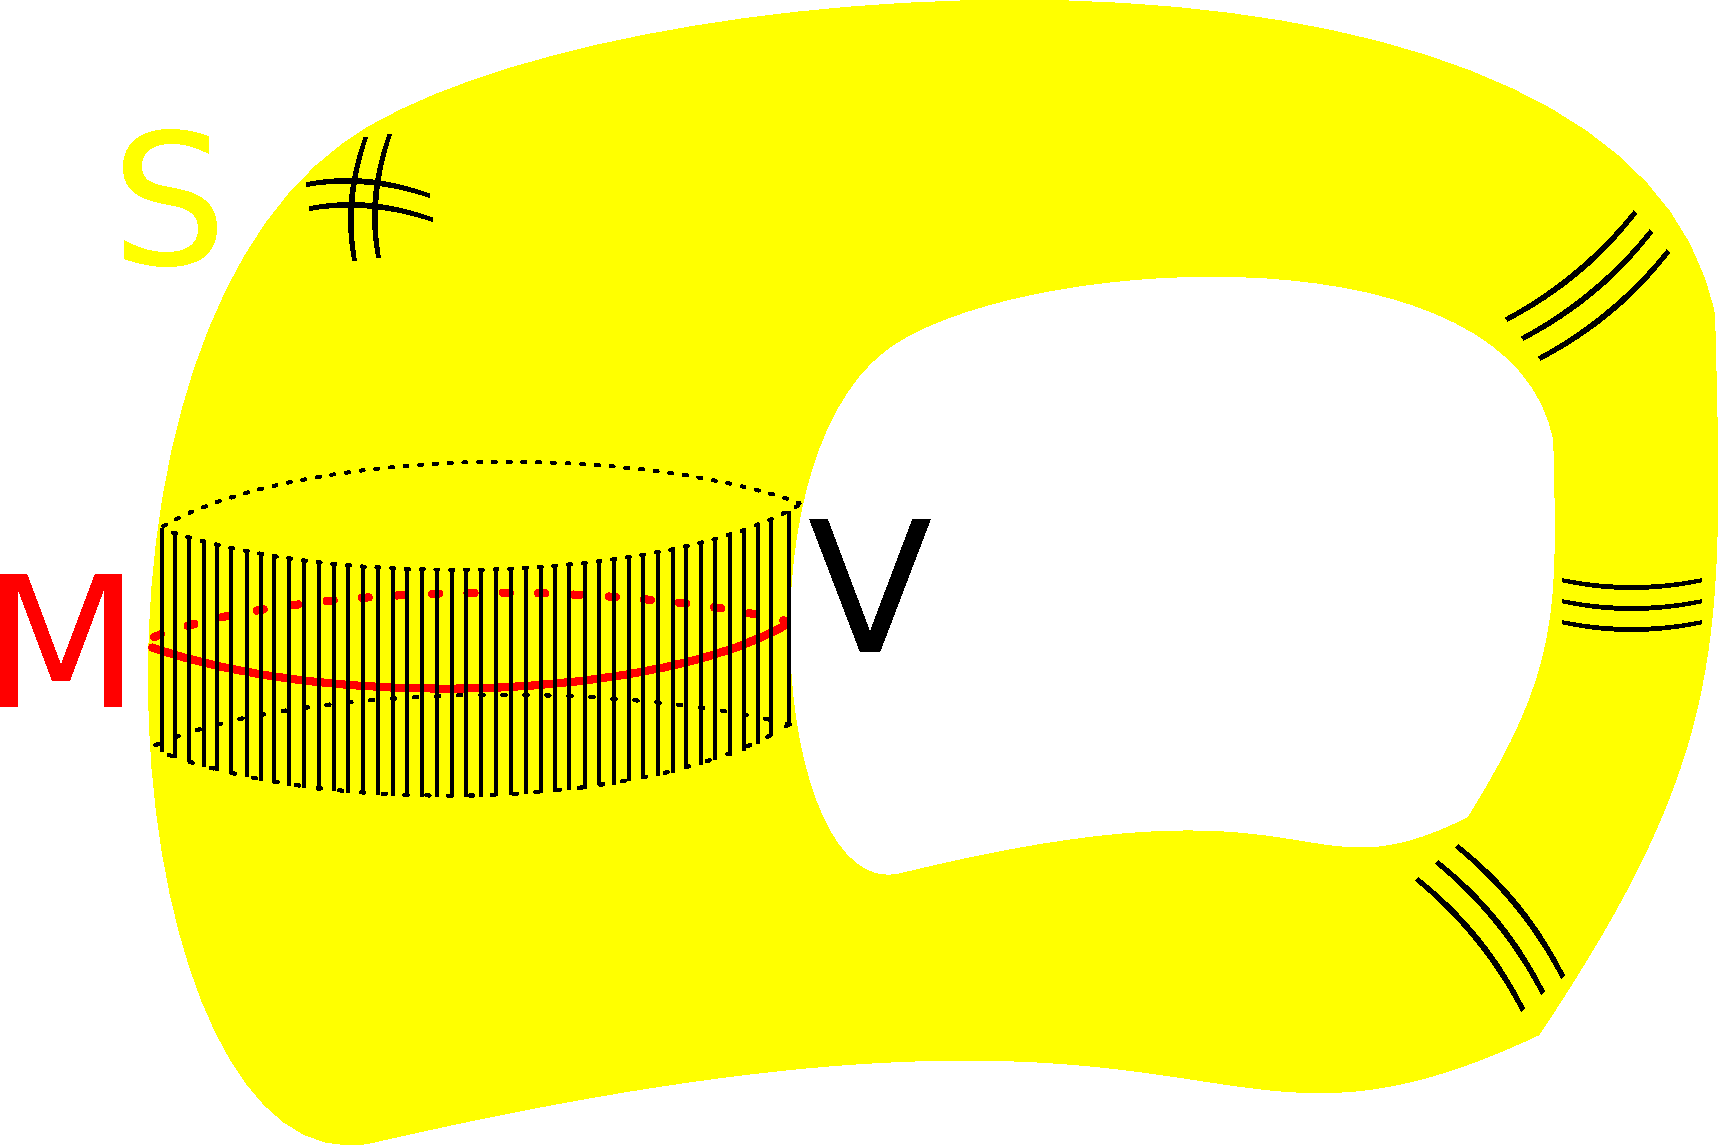
\includegraphics[scale=0.25]{viz_tub.pdf}
    	\caption{Tubular neighborhood of a smooth embedding.}
    \end{figure}

    With that, the proof by Stong in (\cite{stong}, Lemma 7, p. 274) essentially consists of finding a commutative diagram under the following 
    conditions:

    $$ \xymatrix @C=0.5cm {
    	H^{*}(S;\Z_{2})\tensor H^{*}(S;\Z_{2}) \ar[rr] & & H^{*}(S;\Z_{2}) \\
    	& & \\		 
    	H^{*}(S;\Z_{2})\tensor H^{*}(S,S-V;\Z_{2}) \ar[uu] \ar[rr] \ar[dd] & & H^{*}(S,S-V;\Z_{2}) \ar[uu] \ar@/^1.5cm/[lldddd] \ar[dddd] \\
    	& & \\				
    	H^{*}(V;\Z_{2})\tensor H^{*}(V,\partial V;\Z_{2}) \ar[dd] & & \\
    	& & \\	
    	H^{*}(V,\partial V;\Z_{2}) \ar[rr] & & H^{*}(S;\Z_{2})
    } $$

    \

    Since there is no tubular neighborhood\index{tubular neighborhood} in the topological setting, we circumvent this issue using only 
    results about generalized bundles, in order to construct a similar commutative diagram and thus show that the existence of a tubular 
    neighborhood is not essential to this result, but rather certain algebraic consequences of a local-flat 
    embedding\index{local-flat embedding}.

    Finally, we have the following:

    \begin{teo}\label{ap_wu_8}
	If $i:M^{m}\hookrightarrow S^{m+k}$ is a local-flat\index{embedding!local-flat} embedding between closed and connected topological 
    manifolds\index{manifold!topological}, with trivial $\R^{k}-$generalized normal 
    bundle\index{bundle!generalized!normal}\index{bundle!generalized!trivial}, then $v(M)=i^{*}(v(S))$.
    \end{teo}

    \begin{proof}

        \

        First, let $(\mathcal{N},\mathcal{N}_{0})=(N,N_{0},q,M)$ be the $\R^{k}-$generalized normal bundle\index{bundle!generalized!normal} of 
        the local-flat embedding\index{embedding!local-flat} $i$, and let 
        $f:(N,N_{0})\rightleftarrows (M\times\R^{k},M\times (\R^{k}-\{0\})):g$ be the homotopy equivalences given by the triviality of 
        $(\mathcal{N},\mathcal{N}_{0})$. Also recall that $f$ and $g$ are fiber maps\index{map!fiber}, that is, $p_{1}\circ f=q$ and 
        $q\circ g=p_{1}$.
        
        Let $c:S\hookrightarrow (S,S-M)$ be the canonical inclusion and $\xi:(N,N_{0})\to (S,S-M)$ the map given by $\xi(\omega)=\omega(1)$, 
        which, according to (\cite{fadell_1}, Theorem 7.5, p. 509), induces an isomorphism in the context of singular 
        (co)homology\index{singular (co)homology} with coefficients in $\Z_{2}$.
        
        Thus, for any integer $t\geq 0$, the homomorphisms are well defined:
        $$ B=f_{*}\circ (\xi_{*})^{-1}\circ c_{*}:H_{t}(S;\Z_{2})\to H_{t}(M\times (\R^{k},\R^{k}-\{0\});\Z_{2}) $$
        $$ A=c^{*}\circ (\xi^{*})^{-1}\circ f^{*}:H^{t}(M\times (\R^{k},\R^{k}-\{0\});\Z_{2})\to H^{t}(S;\Z_{2}) $$

        \
        
        Note that the homomorphism $A$ is the cohomological dual of the homomorphism $B$.
        
        Furthermore, we also know that the Künneth formula\index{Künneth formula} ensures that:
        $$ H^{t+k}(M\times (\R^{k},\R^{k}-\{0\});\Z_{2})\cong H^{t}(M;\Z_{2})\tensor H^{k}(\R^{k},\R^{k}-\{0\};\Z_{2}) $$

        \
        
        Then, by letting $(\varphi)=H^{k}(\R^{k},\R^{k}-\{0\};\Z_{2})$, we define the homomorphism 
        $\overline{i}:H^{t}(M;\Z_{2})\to H^{t+k}(S;\Z_{2})$ by $\overline{i}(x)=A(x\times \varphi)$.

        \
        
        With the above notations fixed, let us begin the proof.
        
        If we denote $(\sigma)=H_{k}(\R^{k},\R^{k}-\{0\};\Z_{2})$, then $B([S])=[M]\times\sigma$. Indeed, observe that:
        $$ B([S])\in H_{m+k}(M\times (\R^{k},\R^{k}-\{0\});\Z_{2})\cong H_{m}(M;\Z_{2})\tensor H_{k}(\R^{k},\R^{k}-\{0\};\Z_{2})\cong \Z_{2} $$
        
        \
        
        Since $H_{m}(M;\Z_{2})$ and $H_{k}(\R^{k},\R^{k}-\{0\};\Z_{2})$ are generated by $[M]$ and $\sigma$, respectively, then 
        $H_{m}(M;\Z_{2})\tensor H_{k}(\R^{k},\R^{k}-\{0\};\Z_{2})$ is generated by $[M]\tensor\sigma$. That is, the only nonzero class of 
        $H_{m+k}(M\times (\R^{k},\R^{k}-\{0\});\Z_{2})$ is $[M]\times\sigma$.
        
        Therefore, in order to ensure $B([S])=[M]\times\sigma$, it is enough to prove that $B([S])\neq 0$. On the other hand, since 
        $B=f_{*}\circ (\xi_{*})^{-1}\circ c_{*}$ and both $f_{*}$ and $\xi_{*}$ are isomorphisms, we have $B([S])\neq 0$ if and only if 
        $c_{*}([S])\neq 0$.

        \
        
        Now, for an arbitrary point $b\in M\subset S$, the inclusion $j_{b}:S\hookrightarrow (S,S-\{b\})$ can be decomposed as the following 
        inclusions:
        $$ \xymatrix @C=0.5cm {
        	S \ar@{^(->}[rr]^-{c} && (S,S-M) \ar@{^(->}[rr] && (S,S-\{b\})
        } $$

        \
        
        Since $(j_{b})_{*}$ is an isomorphism\footnote{See Proposition \ref{orient_local}.}, $c_{*}$ is a monomorphism and hence 
        $c_{*}([S])\neq 0$ since $[S]\neq 0$.
        
        Therefore, $B([S])=[M]\times\sigma$.
        
        Let us now show that, by defining $e=\xi\circ g:M\times (\R^{k},\R^{k}-\{0\})\to (S,S-M)$, the following diagram commutes for all 
        $t\geq 0$:
        $$ \xymatrix @C=0.5cm {
        	H^{m-t}(S;\Z_{2})\tensor H^{t+k}(S;\Z_{2}) \ar[r]^-{\ccup} & H^{m+k}(S;\Z_{2}) \\
        	& \\		 
        	H^{m-t}(S;\Z_{2})\tensor H^{t+k}(S,S-M;\Z_{2}) \ar[uu]^-{1\times c^{*}} \ar[r]^-{\ccup} \ar[dd]^-{i^{*}\times e^{*}} & H^{m+k}(S,S-M;\Z_{2}) \ar[uu]^-{c^{*}} \ar@/^2cm/[ldddd]^-{e^{*}} \ar[dddd]^-{c^{*}} \\
        	& \\				
        	H^{m-t}(M\times\R^{k};\Z_{2})\tensor H^{t+k}(M\times (\R^{k},\R^{k}-\{0\});\Z_{2}) \ar[dd]^-{\ccup} & \\
        	& \\	
        	H^{m+k}(M\times (\R^{k},\R^{k}-\{0\});\Z_{2}) \ar[r]^-{A} & H^{m+k}(S;\Z_{2})
        } $$

        \

        Let us prove this commutativity step by step. Initially, due to the very definitions of the homomorphisms $A$ and $e^{*}$, it is clear 
        that $A\circ e^{*}=c^{*}$.

        On the other hand, Lemma \ref{propriedades_produtos_2} ensures that the inclusion $c:S\hookrightarrow (S,S-M)$ satisfies the property 
        that $c^{*}(x\ccup y)=x\ccup c^{*}(y)$ for any $x\in H^{m-t}(S;\Z_{2})$ and $y\in H^{t+k}(S,S-M;\Z_{2})$.

        Now, we can assume, without loss of generality, that the embedding $i:M\hookrightarrow S$ induces 
        $i^{*}:H^{t}(S;\Z_{2})\to H^{t}(M\times\R^{k};\Z_{2})$, since $\R^{k}$ is a contractible topological space. Moreover, we can take this 
        contraction as $M\to M\times \R^{k}$ that maps $b\mapsto (b,0)$.

        Thus, in order to restrict the image of $e:M\times(\R^{k},\R^{k}-\{0\})\to (S,S-M)$ to $S$, it is necessary to restrict the domain to 
        $M\times \{0\}$. In this way, the restriction $e_{|M\times\{0\}}:M\times\{0\}\to S$ reduces to the embedding $i$, since for a fixed 
        $b\in M$, $g(b,0)\in N-N_{0}$ is the constant path in $S$ equal to $b\in M$, and thus:

        \

        $ \begin{array}{rl}
        	e(b,0) \ = & \xi\circ g(b,0) \\
        	= &   \\
        	= & b \\
        	= & i(b)
        \end{array} $

        \

        Hence, we obtain for any $x\in H^{m-t}(S;\Z_{2})$ and $y\in H^{t+k}(S,S-M;\Z_{2})$ that $e^{*}(x\ccup y)=i^{*}(x)\ccup e^{*}(y)$.

        With this, the diagram shown above is indeed commutative.

        \
        
        Moreover, recalling that $\overline{i}:H^{t}(M;\Z_{2})\to H^{t+k}(S;\Z_{2})$ is the homomorphism defined by 
        $\overline{i}(x)=A(x\times \varphi)$, where $\varphi\in H^{k}(\R^{k},\R^{k}-\{0\};\Z_{2})$, we can obtain for any 
        $x\in H^{t}(M;\Z_{2})$ and $y\in H^{m-t}(S;\Z_{2})$ that:

        \

        $ \begin{array}{rl}
        	A(i^{*}(y)\ccup (x\times\varphi)) \ = & y\ccup c^{*}((e^{*})^{-1}(x\times\varphi)) \\
        	= & y\ccup A(x\times\varphi) \\
        	= & y\ccup \overline{i}(x)
        \end{array} $

        \

        Therefore, we have for any $x\in H^{t}(M;\Z_{2})$ and $y\in H^{m-t}(S;\Z_{2})$ that:

        \

        $ \begin{array}{rl}
        	<\overline{i}(x)\ccup y,[S]> \ = & <A(i^{*}(y)\ccup (x\times\varphi)),[S]> \\
        	= & <i^{*}(y)\ccup (x\times\varphi),B([S])> \\
        	= & <i^{*}(y),([M]\times\sigma)\ccap (x\times\varphi)> \\
        	= & <i^{*}(y),([M]\ccap x)\times (\sigma\ccap\varphi)> \\
        	= & <i^{*}(y),[M]\ccap x> \\
        	= & <x\ccup i^{*}(y),[M]>
        \end{array} $

        \

        \

        Finally, we are ready to prove that $i^{*}(v(S))=v(M)$. To do so, due to the uniqueness of the Wu classes\index{class!Wu class}, it 
        suffices to show that for all $0\leq t\leq n$:
        $$ <i^{*}(v_{t}(S))\ccup x,[M]>=<Sq^{t}(x),[M]>, \ \forall x\in H^{m-t}(M;\Z_{2}) $$

        \

        But first, note that $Sq^{t}(\varphi)=0$ when $t>0$, since $H^{k+t}(\R^{k},\R^{k}-\{0\};\Z_{2})=0$ for $t>0$ and 
        $Sq^{t}(\varphi)\in H^{k+t}(\R^{k},\R^{k}-\{0\};\Z_{2})$. With this, we obtain that $Sq^{t}(x\times \varphi)=Sq^{t}(x)\times\varphi$, 
        for any $x\in H^{*}(M;\Z_{2})$.

        Thus, we have for any $0\leq t\leq m$ and $x\in H^{m-t}(M;\Z_{2})$ that:

        \

        $ \begin{array}{rl}
        	<i^{*}(v_{t}(S))\ccup x,[M]> \ = & <\overline{i}(x)\ccup v_{t}(S),[S]> \\
        	= & <Sq^{t}(\overline{i}(x)),[S]> \\
        	= & <Sq^{t}(A(x\times\varphi)),[S]> \\
        	= & <A(Sq^{t}(x)\times\varphi),[S]> \\
        	= & <\overline{i}(Sq^{t}(x)),[S]> \\
        	= & <\overline{i}(Sq^{t}(x))\ccup 1,[S]> \\
        	= & <i^{*}(1)\ccup Sq^{t}(x),[M]> \\
        	= & <Sq^{t}(x),[M]>
        \end{array} $

        \

        Therefore, $i^{*}(v(S))=v(M)$.

    \end{proof}

    Thus, we conclude this chapter with several contributions in the context of characteristic classes of topological manifolds. More 
    specifically, we presented maps related to the Stiefel–Whitney\index{class!Stiefel–Whitney}, Euler\index{class!Euler}, and 
    Wu\index{class!Wu} classes of closed topological manifolds.

    Among these contributions, we highlight:

    \begin{itemize}
        \item A second proof of the topological version of the Wu formula\index{formula!Wu}, with some of the preliminary lemmas developed 
        both for $\Z_{2}-$modules and for $\Z-$modules of singular (co)homology\index{singular (co)homology}.
        \item How the preliminary lemmas of the Wu formula allowed us to relate the Euler class\index{class!Euler} and the Euler 
        characteristic of a topological manifold and, consequently, ensure the vanishing of the Euler characteristic of an odd-dimensional 
        topological manifold.
        \item An alternative proof of one direction of the topological version of the Poincaré–Hopf theorem\index{theorem!Poincaré–Hopf}, 
        which shows the relationship between the existence of a nonsingular path field\index{field!path!nonsingular} on a topological manifold 
        and the vanishing of its Euler characteristic\index{Euler characteristic}, using the Euler class in its proof.
        \item How the theory of generalized bundles was essential to relate the Wu classes\index{class!Wu} of topological manifolds via a 
        local-flat embedding\index{embedding!local-flat} with a trivial generalized normal 
        bundle\index{bundle!generalized!normal}\index{bundle!generalized!trivial}.
    \end{itemize}

    Furthermore, with all the results presented so far, we also conclude the importance of generalized bundles\index{bundle!generalized} not 
    only as a tool for the theory of characteristic classes of topological manifolds\index{manifold!topological}, but as a theory in its own 
    right.




    
    \chapter{Characteristic Classes of Generalized Manifolds}\label{cap_wu_gen}
    \thispagestyle{empty}

    \

    In this chapter, we present for the first time in the literature a proof of Wu's formula in the context of generalized 
    manifolds\index{generalized manifold}.

    We begin in Section~\ref{sec_varied_gen} with a brief overview, based on \cite{biasi}, \cite{denise}, and \cite{bredon_2}, of the concept 
    of generalized manifolds, introducing the definition of such an object as well as some of its properties.

    In Section~\ref{sec_thom_gen}, we algebraically construct the Thom class and Thom isomorphism associated to an embedding between 
    generalized manifolds with a specific codimension, following the results presented by Dold in (\cite{dold}, Chapter 8).

    Then, in Section~\ref{sec_SW_gen}, we construct the Stiefel–Whitney classes\index{Stiefel–Whitney class} of embeddings between generalized 
    manifolds with a specific codimension, the Stiefel–Whitney classes of generalized manifolds, and also point out the similarities between 
    these constructions and the topological context presented in Chapter~\ref{cap_clas_carac}.

    Finally, to conclude the chapter, we present in Section~\ref{sec_form_wu_gen} the proof of Wu's formula for generalized manifolds using 
    only their dualities—that is, without requiring the existence of a tangent bundle for such manifolds. The techniques used are based on 
    the results presented by Bredon in (\cite{bredon}, Chapter 6).



    \section{Generalized Manifolds}\label{sec_varied_gen}

    \

    This section aims to present the basic results on generalized manifolds, as well as the formal definition of such objects.

    For a more detailed discussion on generalized manifolds, see \cite{biasi}, \cite{bredon_2}, \cite{mio_1}, \cite{mio_2}, \cite{denise}, 
    and \cite{wilder}.

    We begin the final chapter of this work with the following definitions:

    \begin{defi}{\bf (Cohomological Dimension)\index{cohomological dimension}}\label{defi_dim_coh}
        Let $M$ be a locally compact Hausdorff topological space. We say that $M$ has finite cohomological $\Z_{2}-$dimension, denoted by 
        $dim_{\Z_{2}}M<\infty$\index{dim$_{\Z_{2}}<\infty$}, if there exists an integer $m\geq 0$ such that $H^{m+1}_{c}(U;\Z_{2})=0$ for every 
        open neighborhood $U\subset M$.
    \end{defi}

    Definition~\ref{defi_dim_coh} is, in fact, a consequence concerning the cohomological dimension of a space, whose proof can be found in 
    (\cite{bredon_2}, Theorem 16.14, p. 115).

    \begin{defi}{\bf (Homology Manifold)\index{homology manifold}}
        A locally compact Hausdorff topological space $M$ is called an $m-$dimensional $\Z_{2}-$homology manifold if:
        \begin{itemize}
          \item $dim_{\Z_{2}}M<\infty$;
          \item $\forall b\in M,\ H_{k}(M,M-\{b\};\Z_{2})\cong \left\{ \begin{array}{cl}
            \Z_{2} & ,\ \text{if } k=m \\
            0 & ,\ \text{if } k\neq m
          \end{array}\right.$
        \end{itemize}
    \end{defi}

    \begin{defi}{\bf (Hereditarily Paracompact)\index{hereditarily paracompact}}
        A Hausdorff topological space $M$ is called hereditarily paracompact if every open subset of $M$ is paracompact.
    \end{defi}

    In particular, every metric space is hereditarily paracompact\footnote{For more details on hereditarily paracompact spaces, see 
    (\cite{bredon_2}, Chapter 1, Section 6).}.

    \begin{defi}{\bf (Locally Homologically Connected)\index{locally homologically connected}}
        A topological space $M$ is said to be locally homologically connected, denoted by $HLC_{\Z_{2}}^{\infty}$\index{HLC$_{\Z_{2}}^{\infty}$}, 
        if for every $b\in M$ and every open neighborhood $U\subset M$ of $b$, there exists an open neighborhood $V\subset U$ of $b$ such that the 
        homomorphism $\wt{H}_{k}(V;\Z_{2})\to \wt{H}_{k}(U;\Z_{2})$ induced by the inclusion $V\hookrightarrow U$ is trivial for all integers 
        $k\geq 0$.
    \end{defi}

    \begin{defi}{\bf (Generalized Manifold)\index{generalized manifold}}
        A locally compact Hausdorff topological space $M$ is called an $m-$dimensional $\Z_{2}-$generalized manifold if:
        \begin{enumerate}
          \item $M$ is an $m$-dimensional $\Z_{2}-$homology manifold;
          \item $M$ is hereditarily paracompact;
          \item $M$ is $HLC_{\Z_{2}}^{\infty}$.
        \end{enumerate}
    \end{defi}

    Note that the above definitions can be stated for an arbitrary coefficient group, not necessarily $\Z_{2}$, but since the purpose of this 
    chapter is to work with Stiefel–Whitney and Wu classes, we will restrict ourselves to $\Z_{2}-$generalized manifolds.

    On the other hand, although the definition of a generalized manifold is somewhat complex, these manifolds are well-behaved from an 
    algebraic perspective, as we shall see.

    First, the dimension of a generalized manifold coincides with its cohomological dimension, as shown in the proposition below, whose proof 
    can be found in (\cite{bredon_2}, Remark 9.6, p. 331).

    \begin{prop}
        If $M^{m}$ is a $\Z_{2}-$generalized manifold, then $dim_{\Z_{2}}M=m$.
    \end{prop}

    The singular cohomology modules of generalized manifolds are well-behaved in the following sense:

    \begin{prop}
        If $M^{m}$ is a compact $\Z_{2}-$generalized manifold, then $H^{k}(M;\Z_{2})$ is a finitely generated module for every integer 
        $0\leq k\leq m$.
    \end{prop}

    The proof of the proposition above can be found in (\cite{bredon_2}, Corollary 17.7, p. 129).

    As a matter of curiosity, generalized manifolds differ from topological manifolds starting in dimension three, as we can see in the 
    theorem below, whose proof is found in (\cite{bredon_2}, Theorem 16.32, p. 388).

    \begin{teo}
        Let $M^{m}$ be a second-countable homological manifold\footnote{A topological space is said to be second-countable if it has a countable 
        base.} and suppose $m\leq 2$. Then $M$ is a topological manifold.
    \end{teo}

    Before proceeding, we would like to highlight that there are several studies concerning the existence of generalized manifolds that are 
    not topological manifolds. In fact, there are specific conditions that determine whether a generalized manifold has the same homotopy type 
    as a topological manifold or not. However, since we will not pursue this direction, we suggest \cite{mio_1}, \cite{mio_2}, and 
    \cite{gm-book} for readers interested in this topic.

    Continuing our summary on generalized manifolds, the following result ensures the existence of Poincaré duality in the context of these 
    manifolds, as presented in (\cite{bredon_2}, Corollary 10.2, p. 338), with a statement identical to that of smooth and topological 
    manifolds:

    \begin{teo}
        Consider $M^{m}$ a compact and connected generalized manifold, and let $([M])=H^{m}(M;\Z_{2})\cong\Z_{2}$. Then, for every $k\geq 0$, the 
        duality obtained by homomorphism $\mathcal{D}_{M}:H^{k}(M;\Z_{2})\to H_{m-k}(M;\Z_{2})$, defined by $\mathcal{D}_{M}(x)=[M]\ccap x$, is 
        indeed an isomorphism.
    \end{teo}

    More generally, Halverson proved in (\cite{halverson}, Theorem 5.2, p. 242) that the Poincaré-Hopf duality is also valid for generalized 
    manifolds, with the following statement:

    \begin{teo}
        Let $N^{n}$ be a compact generalized manifold, let $M\subset N$ be a closed subspace, and let $([N]_{M})=H_{n}(N,N-M;\Z_{2})\cong\Z_{2}$ 
        be its generator. Then, for every $k\geq 0$, the homomorphism $\mathcal{D}_{N,M}:\check{H}^{k}(M;\Z_{2})\to H_{n-k}(N,N-M;\Z_{2})$, 
        defined by $\mathcal{D}_{N,M}(x)=[N]_{M}\ccap x$, is indeed an isomorphism.
    \end{teo}

    After these initial considerations about generalized manifolds, we may assume that these objects are, roughly speaking, topological spaces 
    that behave like topological manifolds in the context of singular (co)homology with $\Z_{2}-$module coefficients.

    Moreover, due to some techniques we will use throughout this chapter, we will now work with a particular, yet broad, class of generalized 
    manifolds: homological ENR-manifolds\footnote{The ENR condition is sufficient to ensure that a homological manifold is a generalized 
    manifold.}. To briefly illustrate this class of manifolds that we will work with in this chapter, let us consider an example of a 
    homological ENR-manifold that is not homeomorphic to a topological manifold.

    \begin{ex}
        Let $M^{m}$ be a topological manifold that is not homeomorphic to the sphere $\mathbb{S}^{m}$, but that is a $(\Z_{2},m)-$homology sphere, 
        i.e., $H_{k}(M;\Z_{2})\cong H_{k}(\mathbb{S}^{m};\Z_{2})$ for every integer $k\geq 0$. Then, the suspension $S(M)$ of $M$ is a homological 
        ENR-manifold of dimension $m+1$.

        Indeed, since $M$ is an ENR space, its suspension $S(M)$ is also an ENR. On the other hand, we know that 
        $H_{k}(S(M),S(M)-\{b\};\Z_{2})\cong H_{k}(\R^{m+1},\R^{m+1}-\{0\};\Z_{2})$ for any $b\in S(M)$ and any integer $k\geq 0$, that is, $S(M)$ 
        is a homological manifold.

        However, $S(M)$ is not a topological manifold, because for any open neighborhood $V\subset S(M)$ of the top vertex $v_{+}\in S(M)$ of the 
        suspension, we also know that $V\approx C_{+}(M)$, where $C_{+}(M)$ is the upper cone of the suspension $S(M)$. But $C_{+}(M)$ is not 
        homeomorphic to the disk $D^{m+1}$, since its boundary $\partial(C_{+}(M))=M$ is not homeomorphic to the sphere $\mathbb{S}^{m}$.
    \end{ex}

    The example above is taken from (\cite{denise}, Example 2.2.4, p. 23).



    \section{Thom's Class and Isomorphism}\label{sec_thom_gen}

    \

    In (\cite{dold}, Chapter 8), Dold constructed the Thom class and Thom isomorphism associated with an embedding between topological 
    manifolds using Poincaré and Poincaré-Lefschetz dualities. After examining these constructions more closely, we realized that Dold used 
    only algebraic properties of topological manifolds, which motivated us to attempt the same approach in the context of generalized 
    manifolds\index{manifold!generalized}.

    With some adaptations of the results presented by Dold, we will see in this section how to algebraically construct the Thom 
    class\index{Thom class} and Thom isomorphism\index{Thom isomorphism} associated with a topological embedding\index{embedding!topological}, 
    of specific codimension, between ENR\index{ENR} homology manifolds\index{manifold!homology} using only the 
    Poincaré\index{Poincaré duality} and Poincaré-Lefschetz\index{Poincaré-Lefschetz duality} dualities of these manifolds.

    To that end, we will fix the following assumptions throughout this section:

    \begin{itemize}
        \item $s:M^{m}\to N^{2m}$ is a topological embedding\index{embedding!topological} between compact, connected ENR\index{ENR} homology 
        manifolds\index{manifold!homology};
        \item since we can assume, without loss of generality, that $M\subset N$, we will suppose that $M$ is a retract\index{retract} of $N$, 
        that is, we assume there exists a map $p:N^{2m}\to M^{m}$ such that $p\circ s=1$;
        \item $\mathcal{D}_{M}:H^{k}(M;\Z_{2})\to H_{m-k}(M;\Z_{2})$ is the Poincaré duality\index{Poincaré duality} of $M$, defined by 
        $\mathcal{D}_{M}(x)=[M]\ccap x$;
        \item $\mathcal{D}_{N}:H^{k}(N;\Z_{2})\to H_{2m-k}(N;\Z_{2})$ is the Poincaré duality\index{Poincaré duality} of $N$, defined by 
        $\mathcal{D}_{N}(x)=[N]\ccap x$;
        \item $\mathcal{D}_{N,M}:H^{k}(M;\Z_{2})\to H_{2m-k}(N,N-M;\Z_{2})$ is the Poincaré-Lefschetz 
        duality\index{Poincaré-Lefschetz duality} of $M\subset N$, defined by $\mathcal{D}_{N,M}(x)=[N]_{M}\ccap x$.
    \end{itemize}

    Before proceeding, recall that since every homology manifold is $\Z_{2}-$orientable, there is no obstacle to considering the dualities 
    mentioned above. Also recall that the global orientation classes\index{global orientation class} of $M$ and $N$ are, respectively, the 
    generators $([M])=H_{m}(M;\Z_{2})$ and $([N])=H_{2m}(N;\Z_{2})$, and the local orientation class\index{local orientation class} of $N$ 
    along $M$ is the generator $([N]_{M})=H_{2m}(N,N-M;\Z_{2})$.

    Moreover, by fixing the canonical inclusion $j:N\hookrightarrow (N,N-M)$, we also know that the dualities $\mathcal{D}_{N}$ and 
    $\mathcal{D}_{N,M}$ are related by the following commutative diagram:
    $$ \xymatrix @C=0.5cm {
        H^{k}(N;\Z_{2}) \ar[rr]^-{s^{*}} \ar[ddd]^-{\mathcal{D}_{N}} \ar[rrddd]^-{[N]_{M}\ccap} && H^{k}(M;\Z_{2}) \ar[ddd]^-{\mathcal{D}_{N,M}} \\
        && \\
        && \\
        H_{2m-k}(N;\Z_{2}) \ar[rr]^-{j_{*}} && H_{2m-k}(N,N-M;\Z_{2})
    } $$

    \

    Since $\mathcal{D}_{N}(1)=[N]$ and the diagram above commutes, we conclude the following relation:
    $$ j_{*}([N])=[N]_{M} $$

    Furthermore, the diagram above also ensures the following:

    \begin{lem}\label{lema_tecnico_dualidades}
        Given any $a\in H_{k}(N,N-M;\Z_{2})$, there exists $x\in H^{2m-k}(N;\Z_{2})$ such that $a=[N]_{M}\ccap x$
    \end{lem}
    \begin{proof}

        \ 

        This follows directly from the relation $\mathcal{D}_{N,M}\circ s^{*}(\_)=[N]_{M}\ccap(\_)$ and from the facts that 
        $\mathcal{D}_{N,M}$ is an isomorphism and $s^{*}$ is surjective, since $p\circ s=1$.

    \end{proof}

    Now that we have fixed all necessary notations for the development of the rest of this chapter, let us construct the Thom 
    class\index{Thom class} associated with the embedding $s:M^{m}\to N^{2m}$. To do so, we begin by defining the transfer isomorphism:

    \begin{defi}{\bf (Transfer Isomorphism\index{transfer isomorphism})}
        To the embedding $s:M^{m}\to N^{2m}$ corresponds a natural homomorphism $s_{!}:H_{k}(N,N-M;\Z_{2})\to H_{k-m}(M;\Z_{2})$, called the 
        transfer isomorphism, obtained as a composition of following canonical maps:
        $$ \xymatrix @C=0.5cm {
        s_{!}:H_{k}(N,N-M;\Z_{2}) \ar[rrr]^-{\mathcal{D}^{-1}_{N,M}} &&& H^{2m-k}(M;\Z_{2}) \ar[rrr]^-{\mathcal{D}_{M}} &&& H_{k-m}(M;\Z_{2})
        } $$
    \end{defi}

    \

    Thanks to the transfer isomorphism, we have:

    \

    $H_{k}(N,N-M;\Z_{2}) \ \cong \ \left\{\begin{array}{cl}
    	\Z_{2} & , \ k=m \text{ and } k=2m \\
    	0      & , \ k<m \text{ or } k>2m
    \end{array}\right.$

    \

    Hence, the Universal Coefficient Theorem\index{Universal Coefficient Theorem} guarantees that:

    \

    $H^{k}(N,N-M;\Z_{2}) \ \cong \ \left\{\begin{array}{cl}
    	\Z_{2} & , \ k=m \text{ and } k=2m \\
    	0      & , \ k<m \text{ or } k>2m
    \end{array}\right.$

    \

    \begin{defi}{\bf (Thom class\index{Thom!class})}
    	We call the Thom class associated with the embedding $s:M^{m}\to N^{2m}$ the generator $(\tau_{s})=H^{m}(N,N-M;\Z_{2})$
    \end{defi}

    Let us also note that the transfer isomorphism\index{transfer!isomorphism} $s_{!}$ and the embedding $s$ are related in the following way:

    \begin{lem}\label{lema_tecnico_dualidades_4}
    	For any $x\in H^{k}(N;\Z_{2})$, we have:
    	$$ s_{!}([N]_{M}\ccap x)=[M]\ccap s^{*}(x) $$
    \end{lem}
    \begin{proof}

        \

    	Given any $x\in H^{k}(N;\Z_{2})$ and recalling that $\mathcal{D}_{N,M}\circ s^{*}(x)=[N]_{M}\ccap x$, we conclude:

        \
    
    	$ \begin{array}{rl}
    		s_{!}([N]_{M}\ccap x) \ = & s_{!}\circ \mathcal{D}_{N,M}\circ s^{*}(x) \\
    		= & \mathcal{D}_{M}\circ \mathcal{D}_{N,M}^{-1}\circ \mathcal{D}_{N,M}\circ s^{*}(x) \\
    		= & \mathcal{D}_{M}\circ s^{*}(x) \\
    		= & [M]\ccap s^{*}(x)
    	\end{array} $
    
    \end{proof}

    Now, the following two lemmas will provide a representative in $H^{m}(N;\Z_{2})$ for the Thom class\index{Thom!class} 
    $\tau_{s}\in H^{m}(N,N-M;\Z_{2})$ associated with the embedding $s:M^{m}\to N^{2m}$.

    \begin{lem}\label{lema_tecnico_dualidades_3}
    	There exists a unique nonzero class $U_{s}\in H^{m}(N;\Z_{2})$ such that:
    	$$ s_{*}([M])=[N]\ccap U_{s} $$
    \end{lem}
    \begin{proof}

        \

    	Initially, since $[M]\neq 0$ in $H_{m}(M;\Z_{2})$ and $s_{*}$ is injective (given that $p\circ s=1$), it follows that 
        $s_{*}([M])\neq 0$ in $H_{m}(N;\Z_{2})$.
    
    	Since $\mathcal{D}_{N}:H^{m}(N;\Z_{2})\to H_{m}(N;\Z_{2})$ is an isomorphism, there exists a unique nonzero class 
        $U_{s}\in H^{m}(N;\Z_{2})$ such that $\mathcal{D}_{N}(U_{s})=s_{*}([M])$, that is, $[N]\ccap U_{s}=s_{*}([M])$.
    
    \end{proof}

    \begin{prop}\label{principal}
	    The canonical inclusion $j:N\hookrightarrow (N,N-M)$ satisfies:
	    $$ j^{*}(\tau_{s})=U_{s} $$
    \end{prop}
    \begin{proof}

        \

        Initially, since $U_{s}\neq 0$ in $H^{m}(N;\Z_{2})$ and $\tau_{s}\neq 0$ in $H^{m}(N,N-M;\Z_{2})$, we have 
        $\tau_{s}\ccup\tau_{s}\neq 0$ and $U_{s}\ccup\tau_{s}\neq 0$, both in $H^{2m}(N,N-M;\Z_{2})$. Thus, since 
        $H^{2m}(N,N-M;\Z_{2})\cong\Z_{2}$, we get:
        $$ (\tau_{s}\ccup\tau_{s})=H^{2m}(N,N-M;\Z_{2})=(U_{s}\ccup\tau_{s}) $$

        \

        Also, since $([N]_{M})=H_{2m}(N,N-M;\Z_{2})\cong\Z_{2}$, then:
        $$ <\tau_{s}\ccup\tau_{s},[N]_{M}> \ = \ 1 \ = \ <U_{s}\ccup\tau_{s},[N]_{M}> $$

        \

        Now, let us prove that $j^{*}(\tau_{s})\neq 0$. To that end, observe:

        \

        $\begin{array}{rl}
        	<j^{*}(\tau_{s}),[N]_{M}\ccap \tau_{s}> \ = & <j^{*}(\tau_{s})\ccup\tau_{s},[N]_{M}> \\
        	= & <j^{*}(\tau_{s})\ccup\tau_{s},j_{*}([N])> \\
        	= & <j^{*}(j^{*}(\tau_{s})\ccup\tau_{s}),[N]> \\
        	= & <j^{*}(\tau_{s})\ccup j^{*}(\tau_{s}),[N]> \\
        	= & <j^{*}(\tau_{s}\ccup\tau_{s}),[N]> \\
        	= & <\tau_{s}\ccup\tau_{s},j_{*}([N])> \\
        	= & <\tau_{s}\ccup\tau_{s},[N]_{M}> \\
        	= & 1
        \end{array}$

        \

        On the other hand, if $j^{*}(\tau_{s})=0$, we would have $<j^{*}(\tau_{s}),[N]_{M}\ccap \tau_{s}>=0$, which is a contradiction. 
        Therefore, $j^{*}(\tau_{s})\neq 0$.

        Thus, the Proposition \ref{prop_alg_comut} ensures that there exists a unique class $x\in H^{m}(N;\Z_{2})$ with 
        $x\neq 0$ such that $<x,\mathcal{D}_{N}(j^{*}(\tau_{s}))>=1$.

        \
        
        If we prove that $<U_{s},\mathcal{D}_{N}(j^{*}(\tau_{s}))>=1=<j^{*}(\tau_{s}),\mathcal{D}_{N}(j^{*}(\tau_{s}))>$, we conclude by 
        uniqueness that $j^{*}(\tau_{s})=U_{s}$. Let us do that:

        $\begin{array}{rl}
        	<U_{s},\mathcal{D}_{N}(j^{*}(\tau_{s}))> \ = & <U_{s},[N]\ccap j^{*}(\tau_{s})> \\
        	= & <U_{s}\ccup j^{*}(\tau_{s}),[N]> \\
        	= & <j^{*}(U_{s}\ccup\tau_{s}),[N]> \\
        	= & <U_{s}\ccup\tau_{s},j_{*}([N])> \\
        	= & <U_{s}\ccup\tau_{s},[N]_{M}> \\
        	= & 1
        \end{array}$

        \

        On the other hand:

        \

        $\begin{array}{rl}
        	<j^{*}(\tau_{s}),\mathcal{D}_{N}(j^{*}(\tau_{s}))> \ = & <j^{*}(\tau_{s}),[N]\ccap j^{*}(\tau_{s})> \\
        	= & <j^{*}(\tau_{s})\ccup j^{*}(\tau_{s}),[N]> \\
        	= & <j^{*}(\tau_{s}\ccup\tau_{s}),[N]> \\
        	= & <\tau_{s}\ccup\tau_{s},j_{*}([N])> \\
        	= & <\tau_{s}\ccup\tau_{s},[N]_{M}> \\
        	= & 1
        \end{array}$

        \

        Therefore, $j^{*}(\tau_{s})=U_{s}$.

    \end{proof}

    Thus, we only need to prove a few more technical results about the Thom class\index{class!Thom} so that we can finally define the Thom 
    isomorphism.

    \begin{lem}\label{lema_tecnico_dualidades_2}
    	$s_{*}([M]) = [N]_{M} \ccap \tau_{s}$
    \end{lem}
    \begin{proof}

    	It suffices to combine Lemma \ref{lema_tecnico_dualidades_3}, Proposition \ref{principal}, and Lemma \ref{propriedades_produtos_3} as 
        follows:

        \

    	$\begin{array}{rl}
    		s_{*}([M]) \ = & [N] \ccap U_{s} \\
    		= & [N] \ccap j^{*}(\tau_{s}) \\
    		= & j_{*}([N]) \ccap \tau_{s} \\
    		= & [N]_{M} \ccap \tau_{s}
    	\end{array}$

    \end{proof}

    \begin{prop}
    	For any $a \in H_{k}(N, N - M; \Z_{2})$, we have:
    	$$ s_{*} \circ s_{!}(a) = a \ccap \tau_{s} $$
    \end{prop}
    \begin{proof}

        \

    	First, we know from Lemma \ref{lema_tecnico_dualidades} that for any $a \in H_{k}(N, N - M; \Z_{2})$, there exists 
        $x \in H^{2m - k}(N; \Z_{2})$ such that $a = [N]_{M} \ccap x$.

    	Thus, Lemmas \ref{lema_tecnico_dualidades_4} and \ref{lema_tecnico_dualidades_2} ensure that:

        \

    	$\begin{array}{rl}
    		s_{*} \circ s_{!}(a) \ = & s_{*} \circ s_{!}([N]_{M} \ccap x) \\
    		= & s_{*}([M] \ccap s^{*}(x)) \\
    		= & s_{*}([M]) \ccap x \\
    		= & \left( [N]_{M} \ccap \tau_{s} \right) \ccap x \\
    		= & [N]_{M} \ccap \left( \tau_{s} \cup x \right) \\
    		= & [N]_{M} \ccap \left( x \cup \tau_{s} \right) \\
    		= & \left( [N]_{M} \ccap x \right) \ccap \tau_{s} \\
    		= & a \ccap \tau_{s}
    	\end{array}$

    \end{proof}

    \begin{teo}
        The transfer isomorphism\index{isomorphism!transfer} $s_{!}: H_{k}(N, N - M; \Z_{2}) \to H_{k - m}(M; \Z_{2})$ can be decomposed as 
        follows:
        $$ \xymatrix @C=0.5cm {
        	s_{!}: H_{k}(N, N - M; \Z_{2}) \ar[rr]^-{\ccap \tau_{s}} && H_{k - m}(N; \Z_{2}) \ar[rr]^-{p_{*}} && H_{k - m}(M; \Z_{2})
        } $$
    \end{teo}

    \begin{proof}

        Given any $a \in H_{k}(N, N - M; \Z_{2})$ and recalling that $p \circ s = 1$, the previous proposition ensures that:

        \

        $\begin{array}{rl}
        	p_{*}(a \ccap \tau_{s}) \ = & p_{*} \circ s_{*} \circ s_{!}(a) \\
        	= & s_{!}(a)
        \end{array}$

    \end{proof}

    \begin{teo}{\bf (Thom isomorphism\index{isomorphism!Thom})}\label{iso_thom_vg}
        For any integer $k \geq 0$, the following composition is an isomorphism:
        $$ \xymatrix @C=0.5cm {
        	\phi_{s}: H^{k}(M; \Z_{2}) \ar[rr]^-{p^{*}} && H^{k}(N; \Z_{2}) \ar[rr]^-{\ccup \tau_{s}} && H^{k + m}(N, N - M; \Z_{2})
        } $$
    \end{teo}

    \begin{proof}

        \

        First, note that for any $a \in H_{k + m}(N, N - M; \Z_{2})$ and $x \in H^{k}(M; \Z_{2})$, we have:

        \

        $\begin{array}{rl}
        	<\phi_{s}(x), a> \ = & <p^{*}(x) \ccup \tau_{s}, a> \\
        	= & <p^{*}(x), a \ccap \tau_{s}> \\
        	= & <x, p_{*}(a \ccap \tau_{s})> \\
        	= & <x, s_{!}(a)>
        \end{array}$

        \

        Thus, $\phi_{s}$ is the cohomological dual of $s_{!}$, and since $s_{!}$ is an isomorphism, the Universal Coefficient 
        Theorem\index{theorem!Universal Coefficient} ensures that $\phi_{s}$ is an isomorphism.

    \end{proof}

    \begin{defi}
        The isomorphism $\phi_{s}: H^{k}(M; \Z_{2}) \to H^{k + m}(N, N - M; \Z_{2})$ described in Theorem \ref{iso_thom_vg} is referred to as the 
        Thom isomorphism\index{isomorphism!Thom} associated with the embedding $s: M^{m} \to N^{2m}$.
    \end{defi}
    


    \section{Stiefel-Whitney Classes}\label{sec_SW_gen}

    \

    We will construct in this section, in a fully algebraic way, the Stiefel–Whitney classes\index{class!Stiefel–Whitney} of embeddings 
    between homological manifolds\index{manifold!homological} and the Stiefel–Whitney classes of homological manifolds. Moreover, using 
    technical results obtained by Fadell in \cite{fadell_1}, we will show some similarities between these constructions and the Stiefel–Whitney 
    classes of $\R^{n}-$generalized normal bundles\index{bundle!generalized!normal} of local-flat embeddings\index{embedding!local-flat} and 
    the Stiefel–Whitney classes of topological manifolds presented in Chapter \ref{cap_clas_carac}.

    Initially, since we can associate to each topological embedding\index{embedding!topological} between homological 
    manifolds\index{manifold!homological}, under specific conditions, its Thom class\index{class!Thom} and Thom 
    isomorphism\index{isomorphism!Thom}, it is possible to define the Stiefel–Whitney classes\index{class!Stiefel–Whitney} of this embedding 
    in a way analogous to what was done for vector bundles\index{bundle!vector} in (\cite{milnor_1}, Chapter 4) and for generalized 
    bundles\index{bundle!generalized} in Chapter \ref{cap_clas_carac}, as follows:

    \begin{defi}{\bf (Stiefel–Whitney classes)\index{class!Stiefel–Whitney}}\label{defi_SW_merg}
    Let $s: M^{m} \to N^{2m}$ be a topological embedding between compact, connected ENR-homological manifolds such that $M$ is a 
    retract\index{retract} of $N$. Denoting by $\tau_{s}$ and $\phi_{s}$ the Thom class and Thom isomorphism associated to the embedding $s$, 
    respectively, we define the $k$-th Stiefel–Whitney class of the embedding $s$ as:
    $$ w_{k}(s) = \phi_{s}^{-1} \circ Sq^{k}(\tau_{s}) \in H^{k}(M; \Z_{2}) $$

    \

    Furthermore, we call $W(s) = \ds\sum_{k \geq 0} w_{k}(s) \in H^{*}(M; \Z_{2})$ the total Stiefel–Whitney 
    class\index{class!Stiefel–Whitney!total} of $s$.
    \end{defi}

    Due to the properties of Steenrod squares, the following result is analogous to Theorem \ref{res_SW_fht_1}.

    \begin{prop}
        If $s: M^{m} \to N^{2m}$ is a topological embedding between compact, connected ENR-homological manifolds such that $M$ is a 
        retract\index{retract} of $N$, then $w_{0}(s) = 1$ and $w_{k}(s) = 0$ for $k > m$. In other words, 
        $W(s) = 1 + \ds\sum_{k = 1}^{m} w_{k}(s)$.
    \end{prop}

    Now, since every local-flat embedding is a topological embedding and every topological manifold is an ENR-homological manifold, we obtain 
    the following:

    \begin{teo}\label{SW_normal_gen}
        Let $s: M^{m} \to S^{2m}$ be a local-flat embedding\index{embedding!local-flat} between closed, connected topological manifolds such that 
        $M$ is a retract\index{retract} of $S$, and let $(\mathcal{N}, \mathcal{N}_{0})$ be its $\R^{m}-$generalized normal 
        bundle\index{bundle!generalized!normal}. If $W(\mathcal{N}, \mathcal{N}_{0})$ and $W(s)$ denote, respectively, the total Stiefel–Whitney 
        classes\index{class!Stiefel–Whitney!total} defined in Definitions \ref{defi_SW_top} and \ref{defi_SW_merg}, then 
        $W(\mathcal{N}, \mathcal{N}_{0}) = W(s)$.
    \end{teo}

    \begin{proof}

        \

        Initially, recall that the normal $\R^{m}-$generalized bundle of the local-flat embedding $s: M \to S$ is the pair 
        $(\mathcal{N}, \mathcal{N}_{0}) = (N, N_{0}, q, M)$\footnote{In this chapter, the letter $N$ will not denote a manifold except in the 
        proof of Theorem \ref{SW_normal_gen}.}, where:

        	\begin{itemize}
        		\item $N_{0} = \{ \omega \in S^{I} \ : \ \omega(t) \in M \Leftrightarrow t = 0 \}$
        		\item $N = N_{0} \cup \{ \omega \in S^{I} \ : \ \omega(t) = \omega(0) \in M, \ \forall t \in I \}$
        		\item $q: N \to M$ is given by $q(\omega) = \omega(0)$
        	\end{itemize}

            \

        Since $s: M \to S$ is a local-flat embedding, denote by $\tau \in H^{m}(N, N_{0}; \Z_{2})$ and 
        $\phi: H^{k}(M; \Z_{2}) \to H^{k+m}(N, N_{0}; \Z_{2})$ the Thom class and Thom isomorphism, respectively, of 
        $(\mathcal{N}, \mathcal{N}_{0})$, where $\phi(x) = q^{*}(x) \smile \tau$.

        On the other hand, considering $s: M \to S$ as a topological embedding\index{embedding!topological} between compact, connected 
        ENR\index{ENR} homological manifolds such that $M$ is a retract of $S$, let $p: S \to M$ be such a retraction\index{retraction} and 
        denote by $\tau_{s} \in H^{m}(S, S - M; \Z_{2})$ the Thom class\index{class!Thom} and 
        $\phi_{s}: H^{k}(M; \Z_{2}) \to H^{k+m}(S, S - M; \Z_{2})$ the Thom isomorphism\index{isomorphism!Thom}, both associated to the 
        embedding $s$, where $\phi_{s}(x) = p^{*}(x) \smile \tau_{s}$.

        Now, defining $\xi: (N, N_{0}) \to (S, S - M)$ by $\xi(\omega) = \omega(1)$, then (\cite{fadell_1}, Theorem 7.5, p. 509) guarantees 
        that $\xi$ induces an isomorphism in the context of $\Z_{2}-$modules of singular cohomology such that $\xi^{*}(\tau_{s}) = \tau$.

        Moreover, since $N - N_{0} = \{ \omega \in S^{I} \ : \ \omega(t) = \omega(0) \in M, \ \forall t \in I \}$, we can consider the 
        restriction $\xi_{|N - N_{0}}: (N - N_{0}) \to (S - (S - M))$ defined by:

        \

        $\begin{array}{rl}
        	\xi_{|N - N_{0}}(\omega) \ = & \omega(1) \\
        							 = & \omega(0) \\
        							 = & q(\omega)
        \end{array}$

        \

        Thus, we have that $\xi^{*} \circ \phi_{s} = \phi$. Indeed:

        \

        $\begin{array}{rl}
        	\forall k \geq 0, \ \forall x \in H^{k}(M; \Z_{2}), \ \xi^{*} \circ \phi_{s}(x) \ = & \xi^{*}\left( p^{*}(x) \smile \tau_{s} \right) \\
        	 = & q^{*}(x) \smile \xi^{*}(\tau_{s}) \\
        	 = & q^{*}(x) \smile \tau \\
        	 = & \phi(x)
        \end{array}$

        \

        Hence, the following diagram is commutative for any integer $k \geq 0$:
        $$ \xymatrix @C=0.5cm {
        	H^{m}(S, S - M; \Z_{2}) \ar[dd]^-{\xi^{*}} \ar[rr]^-{Sq^{k}} && H^{k+m}(S, S - M; \Z_{2}) \ar[dd]^-{\xi^{*}} \ar[rrd]^-{\phi_{s}^{-1}} && \\
        	&& && H^{k}(M; \Z_{2}) \\
        	H^{m}(N, N_{0}; \Z_{2}) \ar[rr]^-{Sq^{k}} && H^{k+m}(N, N_{0}; \Z_{2}) \ar[rru]^-{\phi^{-1}} &&
        } $$

        \

        Therefore, for all $k \geq 0$, we have:

        \

        $ \begin{array}{rl}
        	w_{k}(\mathcal{N}, \mathcal{N}_{0}) \ = & \phi^{-1} \circ Sq^{k}(\tau) \\
        	= & \phi^{-1} \circ Sq^{k} \circ \xi^{*}(\tau_{s}) \\
        	= & \phi^{-1} \circ \xi^{*} \circ Sq^{k}(\tau_{s}) \\
        	= & \phi_{s}^{-1} \circ Sq^{k}(\tau_{s}) \\
        	= & w_{k}(s)
        \end{array} $

    \end{proof}

    Note that, even though there is no notion of tangent bundle for homology manifolds, it is possible to define the Stiefel-Whitney classes 
    of such manifolds as follows:

    \begin{defi}{\bf (Stiefel-Whitney Classes\index{class!Stiefel-Whitney})}\label{defi_SW_hom}
        Let $M^{m}$ be a compact connected homology ENR\index{ENR} manifold. Since the diagonal map\index{map!diagonal} $d:M\to M\times M$ is a 
        topological embedding\index{embedding!topological} and the canonical projection $p_{1}:M\times M\to M$ is a retraction\index{retraction} 
        of $M\times M$ onto $M$, we can then define the total Stiefel-Whitney class\index{class!total Stiefel-Whitney} of $M$ by $W(M)=W(d)$.
    \end{defi}

    For the construction of the Stiefel-Whitney classes of a homology manifold\index{manifold!homology} to be indeed well-defined, we must pay 
    attention to the following point: since every topological manifold is a homology manifold, the construction of the Stiefel-Whitney classes 
    of a topological manifold must be the same regardless of whether we use the construction given by Fadell for topological 
    manifolds\index{manifold!topological} as in Definition \ref{defi_SW_top} or our construction for generalized manifolds as in 
    Definition \ref{defi_SW_hom}. In other words:

    \begin{teo}\label{SW_tang_gen}
    	Consider $M^{m}$ a closed connected topological manifold, $(\tau M,\tau_{0}M)$ its $\R^{m}-$generalized tangent 
        bundle\index{bundle!generalized!tangent} and $d:M\to M\times M$ the diagonal\index{map!diagonal}. Denoting by $W(\tau M,\tau_{0}M)$ 
        and $W(d)$ the total Stiefel-Whitney classes\index{class!total Stiefel-Whitney} of $M$ given by Definitions \ref{defi_SW_top} and 
        \ref{defi_SW_hom}, respectively, then $W(\tau M,\tau_{0}M)=W(d)$.
    \end{teo}

    \begin{proof}
    
    	\
    
    	Recall that $(\tau M,\tau_{0}M)=(TM,T_{0}M,p,M)$, where $p:TM\to M$ is defined by $p(\omega)=\omega(0)$, and that the canonical 
        projection $p_{1}:M\times M\to M$ is a retraction\index{retraction} of $M\times M$ onto $M$, i.e. $p_{1}\circ d=1$, so fix some 
        notations.
    
    	Since $M^{m}$ is a topological manifold with generalized tangent bundle $(\tau M,\tau_{0}M)$, denote by 
        $\tau\in H^{m}(TM,T_{0}M;\Z_{2})$ and $\phi:H^{k}(M;\Z_{2})\to H^{k+m}(TM,T_{0}M;\Z_{2})$ the Thom class and Thom isomorphism, 
        respectively, of $(\tau M,\tau_{0}M)$, where $\phi(x)=p^{*}(x)\ccup \tau$.
    
    	On the other hand, considering $M^{m}$ as a compact connected homology ENR\index{ENR} manifold, denote 
        $\Delta=d(M)$, $\tau_{d}\in H^{m}(M\times M,M\times M-\Delta;\Z_{2})$ the Thom class\index{class!Thom} and 
        $\phi_{d}:H^{k}(M;\Z_{2})\to H^{k+m}(M\times M,M\times M-\Delta;\Z_{2})$ the Thom isomorphism\index{isomorphism!Thom}, both associated 
        to the embedding $d$, where $\phi_{d}(x)=p_{1}^{*}(x)\ccup\tau_{d}$.
    
    	Now, due to part of the proof of Lemma \ref{lema_tecnico_wu}, we know that defining the map 
        $\psi:(TM,T_{0}M)\to (M\times M,M\times M-\Delta)$ by $\psi(\omega)=(\omega(0),\omega(1))$, then $\psi$ induces an isomorphism in the 
        category of $\Z_{2}-$modules of singular cohomology such that $\psi^{*}(\tau_{d})=\tau$ and $\psi^{*}\circ \phi_{d}=\phi$.
    
    	Thus, the following diagram is commutative for any integer $k\geq 0$:
    	$$ \xymatrix @C=0.5cm {
            H^{m}(M\times M,M\times M-\Delta;\Z_{2}) \ar[dd]^-{Sq^{k}} \ar[rr]^-{\psi^{*}} & & H^{m}(TM,T_{0}M;\Z_{2}) \ar[dd]^-{Sq^{k}} \\
             & & \\
            H^{k+m}(M\times M,M\times M-\Delta;\Z_{2}) \ar[rdd]^-{\phi_{d}^{-1}} \ar[rr]^-{\psi^{*}} & & H^{k+m}(TM,T_{0}M;\Z_{2}) \ar[ldd]^-{\phi^{-1}} \\
             & & \\
             & H^{k}(M;\Z_{2}) &
        } $$

        \
        
        Therefore, for all $k\geq 0$, we have:

        \
    
    	$ \begin{array}{rl}
    		w_{k}(\tau M,\tau_{0}M) \ = & \phi^{-1}\circ Sq^{k}(\tau) \\
    		= & \phi^{-1}\circ Sq^{k}\circ \psi^{*}(\tau_{d}) \\
    		= & \phi^{-1}\circ \psi^{*}\circ Sq^{k}(\tau_{d}) \\
    		= & \phi_{d}^{-1}\circ Sq^{k}(\tau_{d}) \\
    		= & w_{k}(d)
    	\end{array} $
    
    \end{proof}
   


    \section{Wu's Formula for Generalized Manifolds}\label{sec_form_wu_gen}

    \

    In (\cite{bredon}, Chapter 6), Bredon presented an alternative proof of Wu's formula\index{formula!of Wu} for closed, connected smooth 
    manifolds\index{manifold!smooth} using the diagonal map\index{map!diagonal}, Poincaré\index{duality!Poincaré} and 
    Poincaré-Lefschetz\index{duality!Poincaré-Lefschetz} dualities, and some properties arising from the existence of the tangent vector 
    bundle\index{vector bundle!tangent}. Noting that Bredon used algebraic properties related to smooth manifolds and tangent vector bundles, 
    all combined with the diagonal map\index{map!diagonal}, we were motivated to attempt the same for the context of homological manifolds by 
    using the algebraic construction of the Thom class\index{class!Thom} and Thom isomorphism\index{isomorphism!Thom} for these manifolds 
    obtained in section \ref{sec_thom_gen}.

    After some adaptations of the results presented by Bredon, we will prove in this section Wu's formula\index{formula!of Wu} for homological 
    manifolds\index{manifold!homological} without necessarily requiring the existence of a tangent bundle for such manifolds, but only using 
    their dualities.

    To this end, throughout this section, we fix $M^{m}$ as a compact, connected ENR\index{ENR} homological 
    manifold\index{manifold!homological}, $d:M \to M \times M$ the diagonal map\index{map!diagonal}, and the canonical projection 
    $p_{1}: M \times M \to M$ as a retraction\index{retraction} of $M \times M$ onto $M$, i.e., $p_{1} \circ d = 1$.

    Also fixing an arbitrary basis $\{b_{i}\}_{i=1}^{r}$ of $H^{*}(M; \Z_{2})$ and its dual basis\index{dual basis} 
    $\{b^{\#}_{i}\}_{i=1}^{r}$, we can write the class $U_{d} \in H^{m}(M \times M; \Z_{2})$ obtained in Lemma \ref{lema_tecnico_dualidades_3} 
    as follows:

    \begin{lem}\label{u_base_dual}
    	$U_{d} = \ds\sum_{i=1}^{r} (b_{i} \times b_{i}^{\#})$
    \end{lem}
    \begin{proof}

        As $\{b_{i}\}_{i=1}^{r}$ and $\{b^{\#}_{i}\}_{i=1}^{r}$ are bases for $H^{*}(M; \Z_{2})$, then 
        $\{b_{i} \times b_{j}^{\#}\}_{i,j=1}^{r}$ forms a basis for $H^{*}(M \times M; \Z_{2})$. Thus, since 
        $U_{d} \in H^{*}(M \times M; \Z_{2})$, for each $i,j = 1, \ldots, r$ there exists a unique $\alpha_{i,j} \in \Z_{2}$ such that:
        $$ U_{d} = \ds\sum_{i,j=1}^{r} \alpha_{i,j} (b_{i} \times b_{j}^{\#}) $$

        \

        Before proceeding with the proof, note that due to the uniqueness of the dual basis\index{dual basis} as in Theorem \ref{base_dual_2}, 
        the set $\{b^{\#}_{i} \times b_{j}\}_{i,j=1}^{r}$ is the dual basis of $\{b_{i} \times b_{j}^{\#}\}_{i,j=1}^{r}$ in 
        $H^{*}(M \times M; \Z_{2})$, since:

        \

        $ \begin{array}{rl}
        	<(b_{i} \times b_{j}^{\#}) \ccup (b_{i'}^{\#} \times b_{j'}), [M \times M]> \ = & <(b_{i} \ccup b_{i'}^{\#}) \times (b_{j}^{\#} \ccup b_{j'}), [M \times M]> \\
        	= & <b_{i} \ccup b_{i'}^{\#}, [M]> <b_{j}^{\#} \ccup b_{j'}, [M]> \\
             & \\
        	= & \left\{ \begin{array}{cl}
        		1, & i' = i \ \text{and} \ j' = j \\
        		0, & \text{otherwise}
        	\end{array} \right.
        \end{array} $

        \

        Thus, $(b_{i} \times b_{j}^{\#})^{\#} = b_{i}^{\#} \times b_{j}$ for any $i,j=1,\ldots,r$.

        Now, by Corollary \ref{base_dual_3}, we also have:
        $$ U_{d} = \ds\sum_{i,j=1}^{r} (b_{i} \times b_{j}^{\#}) < U_{d} \ccup (b_{i} \times b_{j}^{\#})^{\#}, [M \times M] > $$

        \

        Therefore, Lemma \ref{lema_tecnico_dualidades_3} ensures that for any $i,j=1,\ldots,r$:

        \

        $ \begin{array}{rl}
        	\alpha_{i,j} \ = & < U_{d} \ccup (b_{i} \times b_{j}^{\#})^{\#}, [M \times M] > \\
        	= & < b_{i}^{\#} \times b_{j}, [M \times M] \ccap U_{d} > \\
        	= & < b_{i}^{\#} \times b_{j}, d_{*}([M]) > \\
        	= & < d^{*} (b_{i}^{\#} \times b_{j}), [M] > \\
        	= & < b_{i}^{\#} \ccup b_{j}, [M] > \\
        	= & \left\{ \begin{array}{cl}
        		1, & i = j \\
        		0, & i \neq j
        	\end{array} \right.
        \end{array} $

        \

        Hence, $U_{d} = \ds\sum_{i=1}^{r} (b_{i} \times b_{i}^{\#})$.

    \end{proof}

    \begin{lem}
	    $U_{d}/[M]=1\in H^{0}(M;\Z_{2})\cong\Z_{2}$
    \end{lem}

    \begin{proof}

        \

        Initially, by fixing the basic element $(b_{1})=H^{0}(M;\Z_{2})\cong\Z_{2}$, we have $b_{1}=1$. Thus, it is evident that 
        $<b_{1}^{\#},[M]>=1$. In other words, $(b_{1}^{\#})=H^{m}(M;\Z_{2})\cong\Z_{2}$.

        Still, since $b_{i}\notin H^{0}(M;\Z_{2})$ for $i\neq 1$, it is clear that $b_{i}^{\#}\notin H^{m}(M;\Z_{2})$ when $i\neq 1$.

        Therefore, from the previous lemma we obtain:

        \

        $ \begin{array}{rl}
        	U_{d}/[M] \ = & \left( \ds\sum_{i=1}^{r}(b_{i}\times b_{i}^{\#}) \right)/[M] \\
        	= & \ds\sum_{i=1}^{r}\left[ \left( b_{i}\times b_{i}^{\#} \right)/[M] \right] \\
        	= & \ds\sum_{i=1}^{r}b_{i}<b_{i}^{\#},[M]> \\
        	= & b_{1}<b_{1}^{\#},[M]> \\
        	= & b_{1} \\
        	= & 1
        \end{array} $

    \end{proof}

    Now, combining Lemmas \ref{lema_tecnico_dualidades_3} and \ref{lema_tecnico_dualidades_2} for the embedding $d:M\to M\times M$ and 
    denoting $\Delta=d(M)$, we obtain the following relation:
    $$ [M\times M]\ccap U_{d}=[M\times M]_{\Delta}\ccap \tau_{d} $$

    \

    This induces the following:

    \begin{lem}
    	For every integer $k\geq 0$, we have the following relation:
    	$$ [M\times M]\ccap Sq^{k}(U_{d})=[M\times M]_{\Delta}\ccap Sq^{k}(\tau_{d}) $$
    \end{lem}

    \begin{proof}

        \

        We simply observe that for any $k\geq 0$, Proposition \ref{principal} and Lemma \ref{propriedades_produtos_3} ensure that:

        \

        $\begin{array}{rl}
        	[M\times M]\ccap Sq^{k}(U_{d}) \ = & [M\times M]\ccap Sq^{k}(j^{*}(\tau_{d})) \\
        	= & [M\times M]\ccap j^{*}(Sq^{k}(\tau_{d})) \\
        	= & j^{*}([M\times M])\ccap Sq^{k}(\tau_{d}) \\
        	= & [M\times M]_{\Delta}\ccap Sq^{k}(\tau_{d})
        \end{array}$

    \end{proof}

    Thus, denoting by $\phi_{d}:H^{k}(M;\Z_{2})\to H^{k+m}(M\times M,M\times M-\Delta;\Z_{2})$ the Thom isomorphism\index{isomorphism!Thom} 
    associated to the embedding $d$, which is defined by $\phi_{d}(x)=p_{1}^{*}(x)\ccup\tau_{d}$, and recalling that 
    $w_{k}(M)=\phi^{-1}_{d}\circ Sq^{k}(\tau_{d})$, we obtain a first relation between the Stiefel-Whitney 
    classes\index{class!Stiefel-Whitney} of $M$ and the class $U_{d}$ as follows:

    \begin{lem}
	    For every integer $k \geq 0$, we have the following relation:
	    $$ d_{*}([M] \ccap w_{k}(M)) = [M \times M] \ccap Sq^{k}(U_{d}) $$
    \end{lem}

    \begin{proof}

        \

        Using Lemma \ref{lema_tecnico_dualidades_2} and the previous lemma, and recalling that $p_{1} \circ d = 1$, we obtain for all 
        $k \geq 0$:

        \

        $\begin{array}{rl}
        	d_{*}([M] \ccap w_{k}(M)) \ = & d_{*}([M] \ccap d^{*} \circ p_{1}^{*}(w_{k}(M))) \\
        	= & d_{*}([M]) \ccap p_{1}^{*}(w_{k}(M)) \\
        	= & \left( [M \times M]_{\Delta} \ccap \tau_{d} \right) \ccap p_{1}^{*}(w_{k}(M)) \\
        	= & [M \times M]_{\Delta} \ccap \left( \tau_{d} \ccup p_{1}^{*}(w_{k}(M)) \right) \\
        	= & [M \times M]_{\Delta} \ccap \phi_{d}(w_{k}(M)) \\
        	= & [M \times M]_{\Delta} \ccap Sq^{k}(\tau_{d}) \\
        	= & [M \times M] \ccap Sq^{k}(U_{d})
        \end{array}$

    \end{proof}

    This leads to the following lemma, which shows a more elegant relation between the Stiefel–Whitney classes\index{class!Stiefel–Whitney} 
    of $M$ and the class $U_{d}$.

    \begin{lem}
    	For any integer $k \geq 0$, we have:
    	$$ w_{k}(M) = Sq^{k}(U_{d})/[M] $$
    \end{lem}

    \begin{proof}

        \

        Recalling that $p_{1} \circ d = 1$ and using the previous lemma together with item 2 of Lemma \ref{lema_slant}, we obtain for all 
        $k \geq 0$:

        \

        $\begin{array}{rl}
        	\mathcal{D}_{M}(w_{k}(M)) \ = & (p_{1})_{*} \circ d_{*} \circ \mathcal{D}_{M}(w_{k}(M)) \\
        	= & (p_{1})_{*} \left( d_{*} \left( [M] \ccap w_{k}(M) \right) \right) \\
        	= & (p_{1})_{*} \left( [M \times M] \ccap Sq^{k}(U_{d}) \right) \\
        	= & (p_{1})_{*} \left( \left( [M] \times [M] \right) \ccap Sq^{k}(U_{d}) \right) \\
        	= & [M] \ccap \left( Sq^{k}(U_{d})/[M] \right) \\
        	= & \mathcal{D}_{M}(Sq^{k}(U_{d})/[M])
        \end{array}$

        Therefore, since the Poincaré duality\index{duality!Poincaré} $\mathcal{D}_{M}$ is an isomorphism, we conclude that 
        $w_{k}(M) = Sq^{k}(U_{d})/[M]$.

    \end{proof}

    Therefore, we finally obtain the:

    \begin{teo}{\bf (Wu Formula\index{Wu!formula})}
        Let $M^{m}$ be a compact and connected homological ENR\index{ENR} manifold. Then:
    	$$ W(M)=Sq(v(M)) $$
    \end{teo}

    \begin{proof}

        \

        We must prove that, for every integer $k \geq 0$, we have $w_{k}(M)=\ds\sum_{i+j=k}Sq^{i}(v_{j}(M))$.

        Due to Corollary \ref{base_dual_3} and the very definition of Wu classes\index{Wu!class}, we have:

        \

        $ \begin{array}{rl}
        	v_{j}(M) \ = & \ds\sum_{l=1}^{r}<v_{j}(M)\ccup b_{l}^{\#},[M]>b_{l} \\
        	= & \ds\sum_{l=1}^{r}<Sq^{j}(b_{l}^{\#}),[M]>b_{l}
        \end{array} $

        \

        Thus, by the previous lemma and Lemma \ref{u_base_dual}, we conclude:

        \

        $\begin{array}{rl}
        	w_{k}(M) \ = & Sq^{k}(U_{d})/[M] \\
        	= & Sq^{k}\left( \ds\sum_{l=1}^{r}(b_{l}\times b_{l}^{\#}) \right) / [M] \\
        	= & \ds\sum_{l=1}^{r} \left[ Sq^{k}(b_{l}\times b_{l}^{\#}) / [M] \right] \\
        	= & \ds\sum_{l=1}^{r} \left[ \left( \ds\sum_{i+j=k} \left( Sq^{i}(b_{l})\times Sq^{j}(b_{l}^{\#}) \right) \right) / [M] \right] \\
        	= & \ds\sum_{i+j=k}\ds\sum_{l=1}^{r} \left[ \left( Sq^{i}(b_{l})\times Sq^{j}(b_{l}^{\#}) \right) /[M] \right] \\
        	= & \ds\sum_{i+j=k}\ds\sum_{l=1}^{r}<Sq^{j}(b_{l}^{\#}),[M]>Sq^{i}(b_{l}) \\
        	= & \ds\sum_{i+j=k}Sq^{i}\left( \ds\sum_{l=1}^{r}<Sq^{j}(b_{l}^{\#}),[M]>b_{l} \right) \\
        	= & \ds\sum_{i+j=k}Sq^{i}(v_{j}(M))
        \end{array}$

    \end{proof}

    Thus, we conclude this chapter with entirely original contributions to the theory of characteristic classes of generalized 
    manifolds\index{generalized!manifold}, which, roughly speaking, are topological spaces with no geometric condition that share the same 
    homological and cohomological behavior as topological manifolds. In particular, we showed that the fact that 
    Poincaré\index{Poincaré!duality} and Poincaré–Lefschetz\index{Poincaré–Lefschetz!duality} dualities also hold in the context of 
    generalized manifolds was fundamental to the development of this chapter.

    Even though there is no notion of a normal bundle for topological embeddings\index{topological!embedding} between generalized 
    manifolds\index{generalized!manifold}, we algebraically constructed the Thom class\index{Thom!class} and Thom 
    isomorphism\index{Thom!isomorphism} associated with such embeddings. Hence, we defined the Stiefel–Whitney 
    classes\index{Stiefel–Whitney!class} of these embeddings analogously to both the classical definition and the one presented in 
    Chapter \ref{cap_clas_carac}, using Steenrod squares\index{Steenrod!square}, the Thom isomorphism, and the Thom class.

    Moreover, since every local-flat embedding\index{local-flat!embedding} between topological manifolds can be viewed as a topological 
    embedding between generalized manifolds, we showed that the definition of the Stiefel–Whitney classes of the normal generalized 
    bundle\index{generalized!normal!bundle} of a local-flat embedding coincides with the definition of these classes via the construction in 
    the context of generalized manifolds.

    On the other hand, even though there is no notion of a tangent bundle for generalized manifolds, we constructed the Thom class, 
    Thom isomorphism, and the Stiefel–Whitney classes of a generalized manifold by considering the particular case of the embedding given by 
    the diagonal map\index{diagonal!map} of that manifold. We also showed that the definition of the Stiefel–Whitney classes of the tangent 
    generalized bundle\index{generalized!tangent!bundle} of a topological manifold coincides with the definition of these classes when 
    viewing the manifold as a generalized manifold.

    Since Biasi, Daccach, and Saeki defined in \cite{biasi} the Stiefel–Whitney classes of generalized manifolds using the Wu formula itself 
    and presented several results in this context, we emphasize the originality of Chapter \ref{cap_wu_gen}, where we defined the 
    Stiefel–Whitney classes for generalized manifolds via an alternative approach and proved the Wu formula for such manifolds.

    Thus, we conclude this work with several contributions to the theory of characteristic classes, both for topological and for generalized 
    manifolds.





    \appendix

    \chapter{Singular (Co)homology}\label{ap_(co)_sing}
    \thispagestyle{empty}

    \

    In order to keep this work concise, yet complete and self-explanatory, we will use this appendix as 
    a brief review of some well-known concepts from Algebraic Topology.

    When referring simultaneously to the singular homology and cohomology modules, for convenience, we 
    will simply write singular (co)homology modules\index{singular (co)homology}. Thus, we ask the 
    reader to already be familiar with the concepts of these theories.
    
    \section{Main results}\label{ap_principais_res}
    
    We will use this section to state general results on singular (co)homology that will be useful for 
    the development of this work and for a better understanding of the constructions made in the 
    following sections of this appendix.
    
    \begin{teo}{\bf (Universal Coefficients)\index{theorem!of Universal Coefficients}}
        Let $(X,A)$ be any pair of topological spaces. Then:
        \begin{enumerate}
            \item \textbf{(general case for homology)\footnote{Can be found in (\cite{hatcher}, 
            Corollary 3A.4, p. 264).}} If $H_{k}(X,A;\Z)$ is a free 
            module\footnote{A module is called free if it admits a basis.}\index{module!free} for 
            all $k\geq 0$ or $R$ is a free module, then:
            $$ H_{k}(X,A;R)\cong H_{k}(X,A;\Z)\tensor R, \ \forall k\geq 0 $$
            \item \textbf{(general case for cohomology)\footnote{Can be found in (\cite{hatcher}, 
            Theorem 3.2, p. 195).}} If $H_{k}(X,A;\Z)$ is a free module for all $k\geq 0$, then:
            $$ H^{k}(X,A;R)\cong Hom(H_{k}(X,A;\Z);R), \ \forall k\geq 0 $$
            \item \textbf{(particular case)\footnote{Can be found in (\cite{hatcher}, p. 198).}} 
            If $\mathbb{F}$ is a field, then the Kronecker product ensures that:
            $$ H^{k}(X,A;\F)\cong Hom(H_{k}(X,A;\F);\F), \ \forall k\geq 0 $$
        \end{enumerate}
        For $R=\Z$ in case 2 or $R=\F$ in case 3, the isomorphism is given by the relation 
        $x\in H^{k}(X,A;R)\mapsto\overline{x}(a)=<x,a>\in R$.
    \end{teo}
    
    \begin{teo}{\bf (Künneth Formula)\index{formula!of Künneth}}
        Let $X$ and $Y$ be any topological spaces and $R$ a finitely generated principal ideal 
        domain\index{principal ideal domain}. Then:
        \begin{enumerate}
            \item \textbf{(case for absolute cohomology)\footnote{Can be found in (\cite{spanier}, 
            Theorem 1, p. 249).}} If all the singular homology $R$-modules of $Y$ are finitely 
            generated\index{module!finitely generated}, then:
            $$ H^{k}(X\times Y;R)\cong \ds\bigoplus_{i+j=k}\left[ H^{i}(X;R)\tensor H^{j}(Y;R)\right], \ 
            \forall k\geq 0 $$
            \item \textbf{(case for absolute homology)\footnote{Can be found in (\cite{spanier}, 
            Theorem 10, p. 235).}}
            $$ H_{k}(X\times Y;R)\cong \ds\bigoplus_{i+j=k}\left[ H_{i}(X;R)\tensor H_{j}(Y;R)\right], \ 
            \forall k\geq 0 $$
        \end{enumerate}
    \end{teo}
    
    The proofs of the general cases of the Universal Coefficients Theorem can be found in (\cite{spanier}, 
    Chapter 5, Sections 2 and 5).
    
    The proofs of the Künneth formulas, in their general versions for pairs, can be found in 
    (\cite{spanier}, Chapter 5, Sections 3 and 5).
    
    Now, let us briefly review some properties about the cap\index{product!cap}, cup\index{product!cup}, 
    cross\index{product!cross}, and Kronecker\index{product!Kronecker} products.

    \begin{lem}\label{propriedades_produtos}
        Let $X$, $X'$, $Y$, and $Y'$ be arbitrary topological spaces, $f:X\to X'$ and $g:Y\to Y'$ any 
        maps, $p_{1}:X\times Y\to X$ and $p_{2}:X\times Y\to Y$ the canonical projections, and 
        $d:X\to X\times X$ the diagonal map\index{map!diagonal}. If $a\in H_{q}(X;R)$, $b\in H_{r}(Y;R)$, 
        $x\in H^{i}(X;R)$, $x_{1}\in H^{i_{1}}(X;R)$, $x_{2}\in H^{i_{2}}(X;R)$, $y\in H^{j}(Y;R)$, 
        $y_{1}\in H^{j_{1}}(Y;R)$, $y_{2}\in H^{j_{2}}(Y;R)$, $a'\in H_{q'}(X;R)$, $x'\in H^{i'}(X';R)$, 
        $x'_{1}\in H^{i_{1}'}(X';R)$, $x'_{2}\in H^{i_{2}'}(X';R)$, $y'\in H^{j'}(Y';R)$, then:
    
        \begin{enumerate}
            \item $1\ccup x=x=x\ccup 1$
            \item $0\ccup x=0=x\ccup 0$
            \item $x_{1}\ccup x_{2}=0$ \  $\Longleftrightarrow$ \ $x_{1}=0$ or $x_{2}=0$, when $R=\Z_{2}$
            \item $a\ccap 1=a$
            \item $x_{1}\ccup x_{2}=(-1)^{|x_{1}|.|x_{2}|}(x_{2}\ccup x_{1})$
            \item $(a\ccap x_{1})\ccap x_{2}=a\ccap (x_{2}\ccup x_{1})$
            \item $(x_{1}\times y_{1})\ccup (x_{2}\times y_{2})=(-1)^{|y_{1}|.|x_{2}|}(x_{1}\ccup x_{2})\times (y_{1}\ccup y_{2})$
            \item $(a\times b)\ccap (x\times y)=(-1)^{|a|.(|y|-|b|)}(a\ccap x)\times (b\ccap y)$
            \item $<x_{1}\ccup x_{2},a>=<x_{1},a\ccap x_{2}>$
            \item $<x\times y,a\times b>=(-1)^{|x|.|y|}<x,a>.<y,b>$
            \item $p_{1}^{*}(x)=x\times 1$ and $p_{2}^{*}(y)=1\times y$
            \item $x\times y=p_{1}^{*}(x)\ccup p_{2}^{*}(y)$
            \item $x_{1}\ccup x_{2}=d^{*}(x_{1}\times x_{2})$
            \item $f_{*}(a\ccap f^{*}(x'))=f_{*}(a)\ccap x'$
            \item $(f\times g)^{*}(x'\times y')=f^{*}(x')\times g^{*}(y')$
            \item $f^{*}(x'_{1}\ccup x'_{2})=f^{*}(x'_{1})\ccup f^{*}(x'_{2})$
            \item $<f^{*}(x'),a>=<x',f_{*}(a)>$
            \item $<(f^{*})^{-1}(x),a'>=<x,(f_{*})^{-1}(a')>$, if $f^{*}$ and $f_{*}$ are isomorphisms.
        \end{enumerate}
    \end{lem}
    
    The properties in the lemma above can be found, in their general versions for pairs, in 
    (\cite{spanier}, Chapter 5).
    
    Moreover, item 16 of Lemma \ref{propriedades_produtos} admits a particular case when involving the 
    inclusion map, in the following sense:
    
    \begin{lem}\label{propriedades_produtos_2}
        Let $(X,A)$ and $j:X\hookrightarrow (X,A)$ be an arbitrary pair of topological spaces and the 
        canonical inclusion, respectively. Then, for any $x_{1}\in H^{i_{1}}(X;R)$ and $x_{2}\in H^{i_{2}}(X,A;R)$, 
        we have:
        $$ j^{*}(x_{1}\ccup x_{2})=x_{1}\ccup j^{*}(x_{2}) $$
    \end{lem}
    
    The proof of the lemma above can also be found in (\cite{spanier}, Chapter 5).
    
    That said, item 14 of Lemma \ref{propriedades_produtos} admits the following particular case:

    \begin{lem}\label{propriedades_produtos_3}
        Let $(X,A)$ be any pair of topological spaces and let $j:X\hookrightarrow (X,A)$ be the canonical inclusion. Then, for any 
        $x\in H^{i_{1}}(X,A;R)$ and $a\in H_{i_{2}}(X;R)$, we have:
        $$
        j_{*}(a)\ccap x = a\ccap j^{*}(x)
        $$
    \end{lem}
    
    \begin{proof}

        \

        It suffices to observe that, for any $y\in H^{i_{2}-i_{1}}(X;R)$, we have:

        \
        
        $\begin{array}{rl}
            \langle y, j_{*}(a)\ccap x \rangle & = \langle y\ccup x, j^{*}(a) \rangle \\
            & = \langle j^{*}(y\ccup x), a \rangle \\
            & = \langle y\ccup j^{*}(x), a \rangle \\
            & = \langle y, a\ccap j^{*}(x) \rangle
        \end{array}$

        \

        \
    
        Thus, the Universal Coefficient Theorem ensures that $j_{*}(a)\ccap x = a\ccap j^{*}(x)$.
    \end{proof}
    
    Now, also due to the Universal Coefficient Theorem\index{theorem!Universal Coefficient}, the 
    following result is a direct consequence of (\cite{hungerford}, Theorem 4.11, p. 204):
    
    \begin{prop}\label{prop_alg_comut}
        Let $R=\mathbb{Z}$ or $R=\mathbb{F}$ be any field, and let $(X,A)$ be any pair of topological 
        spaces such that $H_{k}(X,A;R)$ is a finitely generated 
        $R$-module\index{module!finitely generated} for all $k\geq 0$. Then, for any $k\geq 0$, 
        $\alpha\in R$ and $a\in H_{k}(X,A;R)$ with $a\neq 0$, there exists a unique $x\in H^{k}(X,A;R)$ 
        such that $x\neq 0$ and $\langle x, a \rangle = \alpha$.
    \end{prop}
    
    Proceeding, we will construct the cohomology ring of a pair $(X,A)$.
    
    \begin{defi}{\bf (Cohomology Ring)}
        We call $(H^{*}(X,A;R), +, \ccup)$ the cohomology ring\index{cohomology ring} of the pair 
        $(X,A)$ with coefficients in $R$, the set formed by the following formal infinite series:
        $$
        H^{*}(X,A;R) = \{ x = x_{0} + x_{1} + x_{2} + \ldots \ : \ x_{k}\in H^{k}(X,A;R), \ \forall 
        k\geq 0 \}
        $$
        
        Furthermore, given $x = x_{0} + x_{1} + x_{2} + \ldots$ and $y = y_{0} + y_{1} + y_{2} + \ldots$ 
        in $H^{*}(X,A;R)$, the operations that define this ring are given by:
        
        \begin{enumerate}
            \item $x + y = z_{0} + z_{1} + z_{2} + \ldots$, where $z_{k} = x_{k} + y_{k}$ for all 
            $k\geq 0$
            \item $x\ccup y = z_{0} + z_{1} + z_{2} + \ldots$, where $z_{k} = 
            \displaystyle\sum_{i+j=k} x_{i}\ccup y_{j}$ for all $k\geq 0$
        \end{enumerate}
    \end{defi}

    Since the cup product is a commutative operation when $R=\Z_{2}$, then $H^{*}(X,A;\Z_{2})$ will be a commutative ring with identity 
    element $1+0+0+\dots\in H^{*}(X,A;\Z_{2})$.

    \begin{teo}\label{teo_elemento_inversivel}
        The units of the ring $H^{*}(X,A;\Z_{2})$ are elements of the following form:
        $$ x=x_{0}+x_{1}+x_{2}+\dots\in H^{*}(X,A;\Z_{2}) \ : \ x_{0}=1 $$
        
        Furthermore, the inverse of a unit $x=1+x_{1}+x_{2}+\dots$ is the following element:
        $$ x^{-1}=1+x^{-1}_{1}+x^{-1}_{2}+\dots, \quad \text{where} \quad x^{-1}_{k}=\ds\sum_{\stackrel{i+j=k}{i\neq 0}}x_{i}\ccup 
        x^{-1}_{j}, \ \forall k\geq 1 $$
    \end{teo}
    
    The proof of the theorem above can be found in (\cite{alex}, Lemma 6.1, p. 53).
    
    At this point, let us see when a topological space has all its singular (co)homology modules finitely generated and under which conditions 
    we can define the Euler characteristic of an arbitrary topological space.
    
    \begin{prop}
        All singular homology modules of a compact ENR space\footnote{An ENR is a topological space that is a retract\index{retract} of an open 
        neighborhood in some Euclidean space, that is, it can be embedded in some Euclidean space as a retract of an open neighborhood of that 
        Euclidean space. More details about these spaces can be found in (\cite{dold}, Chapter 4, Section 8).}\index{ENR} are finitely 
        generated\index{module!finitely generated}.
    \end{prop}
    
    The proof of the proposition above can be found in (\cite{hatcher}, Corollary A.8, p. 527). As a particular consequence, all singular 
    homology modules of a compact topological manifold are free, since every topological manifold\index{manifold!topological} is an ENR and 
    every finitely generated module is free\index{module!free}. Furthermore, due to the Universal Coefficient Theorem, every singular 
    cohomology module of a compact topological manifold is free.
    
    \begin{defi}{\bf (Euler Characteristic)}
        Let $X$ be a topological space such that there exists an integer $n>0$ such that $H_{k}(X;\Z)=0$ for $k>n$ and $H_{k}(X;\Z)$ is a 
        finitely generated $\Z$-module for every $0\leq k\leq n$. Thus, the Euler characteristic\index{Euler characteristic} of $X$ is given 
        by the following alternating sum:
        $$ \chi(X)=\ds\sum_{k=0}^{n}(-1)^{k}\operatorname{rank}(H_{k}(X;\Z)) $$
    \end{defi}
    
    Due to the Universal Coefficient Theorem\index{theorem!Universal Coefficient Theorem}, the Euler characteristic of a space $X$ under the 
    conditions of the definition above can be computed using singular homology modules with coefficients in any field $\F$ as follows:
    $$ \chi(X)=\ds\sum_{k=0}^{n}(-1)^{k}\dim(H_{k}(X;\F)) $$
    
    To conclude this section, let us make some considerations about the infinite real projective space\index{real projective space!infinite} 
    $\RP^{\infty}$, which will be useful for calculating the Stiefel–Whitney classes\index{class!Stiefel–Whitney} of real projective spaces 
    using the topological version of Wu's formula\index{formula!Wu}.
    
    Denoting by $\RP^{k}$ the $k$-dimensional real projective space\index{real projective space!finite}, we can define the infinite real 
    projective space $\RP^{\infty}$ as the direct limit of the following sequence:
    $$ \RP^{0} \subset \RP^{1} \subset \cdots \subset \RP^{k} \subset \cdots $$
    
    In other words, we have that $\RP^{\infty}=\ds\bigcup_{k\geq 0}\RP^{k}$, endowed with the following topology:
    
    \begin{center}
        "$U$ is an open subset of $\RP^{\infty}$ if and only if $U\cap\RP^{k}$ is an open subset of $\RP^{k}$ for every $k\geq 0$."
    \end{center}
    
    Thus, we can state the following:
    
    \begin{lem}\label{iso_proj}
        The canonical inclusion $i:\RP^{n}\hookrightarrow \RP^{\infty}$ gives rise to an isomorphism 
        $i^{*}:H^{k}(\RP^{\infty};\Z_{2})\to H^{k}(\RP^{n};\Z_{2})$ for every $0\leq k\leq n$.
    \end{lem}
    
    \begin{proof}
    
    First, recall that $\RP^{n+1}$ is a CW-complex\index{CW-complex} with one open cell in each dimension, with $\RP^{k}$ being its 
    $k$-skeleton.
    
    Now, consider $e_{n+1}$ as the open $(n+1)$-dimensional cell of $\RP^{n+1}$ and fix $x\in e_{n+1}$. Then, $\RP^{n+1}-\{ x \}$ is a 
    deformation retract\index{deformation retract} of $\RP^{n}$.
    
    On the other hand, considering, up to homeomorphism, $x\in D^{n+1}\subset e_{n+1}$, then $U=\RP^{n+1}-D^{n+1}$ will be an open subspace 
    of $\RP^{n+1}$ such that:
    $$ \overline{U}\subset \operatorname{int}(\RP^{n+1}-\{ x \})=\RP^{n+1}-\{ x \}. $$
    
    Thus, $\mathbb{S}^{n}=\partial D^{n+1}$ is a deformation retract of $(\RP^{n+1}-\{ x \})-U=D^{n+1}-\{ x \}$, and we also obtain the 
    following excision:
    $$ (\RP^{n+1}-U,(\RP^{n+1}-\{ x \})-U)\hookrightarrow (\RP^{n+1},\RP^{n+1}-\{ x \}). $$
    
    Therefore, we have the following isomorphisms:
    
    \[
    \begin{array}{rl}
    H^{k}(\RP^{n+1},\RP^{n};\Z_{2}) \ \cong & H^{k}(\RP^{n+1},\RP^{n+1}-\{ x \};\Z_{2}) \\[8pt]
    \cong & H^{k}(\RP^{n+1}-U,(\RP^{n+1}-\{ x \})-U;\Z_{2}) \\[8pt]
    \cong & H^{k}(D^{n+1},\mathbb{S}^{n};\Z_{2}) \\[8pt]
    \cong & \left\{
    \begin{array}{cl}
    \Z_{2} & ,\quad k=n+1 \\
    0      & ,\quad k\neq n+1
    \end{array}
    \right.
    \end{array}
    \]
    
    In particular, $H^{k}(\RP^{n+1},\RP^{n};\Z_{2})=0$ for $0\leq k\leq n$. From now on in this proof, fix $0\leq k\leq n$.
    
    Now, we prove by induction on $t\geq 2$ that $H^{k}(\RP^{n+t},\RP^{n};\Z_{2})=0$.
    
    To do so, consider initially the long exact cohomology sequence of the triple\footnote{For more details about the long exact cohomology 
    sequence of a triple, see (\cite{hatcher}, p. 200).} $(\RP^{n+2},\RP^{n+1},\RP^{n})$:
    $$ \cdots \to H^{k}(\RP^{n+2},\RP^{n+1};\Z_{2}) \to H^{k}(\RP^{n+2},\RP^{n};\Z_{2}) \to H^{k}(\RP^{n+1},\RP^{n};\Z_{2}) \to \cdots $$
    
    Since $H^{k}(\RP^{n+2},\RP^{n+1};\Z_{2})=0=H^{k}(\RP^{n+1},\RP^{n};\Z_{2})$, the exactness of the sequence above ensures that 
    $H^{k}(\RP^{n+2},\RP^{n};\Z_{2})=0$.
    
    Thus, assuming $H^{k}(\RP^{n+t_{0}},\RP^{n};\Z_{2})=0$ for some $t_{0}>2$, we similarly obtain that 
    $H^{k}(\RP^{n+(t_{0}+1)},\RP^{n};\Z_{2})=0$, simply by using the long exact cohomology sequence of the triple 
    $(\RP^{n+(t_{0}+1)},\RP^{n+t_{0}},\RP^{n})$.
    
    Therefore, we conclude that $H^{k}(\RP^{n+t},\RP^{n};\Z_{2})=0$ for any $t\geq 0$. Consequently:
    $$ H^{k}(\RP^{\infty},\RP^{n};\Z_{2})=\lim_{\longrightarrow}H^{k}(\RP^{n+t},\RP^{n};\Z_{2})=0. $$
    
    Finally, consider the long exact cohomology sequence of the pair $(\RP^{\infty},\RP^{n})$:
    $$
    \xymatrix @C=0.5cm {
    \cdots \ar[rr] && H^{k}(\RP^{\infty},\RP^{n};\Z_{2}) \ar[rr] && H^{k}(\RP^{\infty};\Z_{2}) \ar[rr]^-{i^{*}} && H^{k}(\RP^{n};\Z_{2}) \ar[rr] && \cdots
    }
    $$
    
    Since $H^{k}(\RP^{\infty},\RP^{n};\Z_{2})=0$ and $H^{k}(\RP^{\infty};\Z_{2})\cong\Z_{2}\cong H^{k}(\RP^{n};\Z_{2})$, then $i^{*}$ is a 
    monomorphism between modules of the same dimension, that is, $i^{*}$ is an isomorphism.
    
    \end{proof}



    \section{Slant Product}\label{ap_slant}

    In this section, we will define a specific product between singular (co)homology modules that will be fundamental in the proof of the Wu 
    formula\index{formula!Wu's formula} for topological\index{manifold!topological} and homological\index{manifold!homological} manifolds.

    This product, which we will later call the slant product, is defined for arbitrary topological spaces using singular (co)homology modules 
    with coefficients in an arbitrary commutative unital ring, and it is also used in the proof of the Wu formula for smooth 
    manifolds\index{manifold!smooth}, as seen in (\cite{milnor_1}, Chapter 11).
    
    For our context, let $R=\Z$ or $R=\Z_{2}$, $X$ and $Y$ be arbitrary topological spaces with $H_{k}(Y;R)$ finitely generated for all 
    $k\geq 0$, and integers $i,j\geq 0$. Thus, define the following homomorphism involving $R$-modules of singular (co)homology:
    $$ H^{i}(X;R)\tensor H^{j}(Y;R)\tensor H_{j}(Y;R)\to H^{i}(X;R) $$
    $$ x\tensor y\tensor b\mapsto <y,b>x $$
    
    Now, the Künneth formula\index{formula!Künneth formula} ensures that $H^{*}(X\times Y;R)\cong H^{*}(X;R)\tensor H^{*}(Y;R)$, and since 
    $H^{*}(X\times Y;R)$ is a ring generated by elements of the form $x\times y$, the following homomorphism is well defined:

    \newpage
    $$ H^{i+j}(X\times Y;R)\tensor H_{j}(Y;R)\to H^{i}(X;R) $$
    $$ (x\times y)\tensor b\mapsto (x\times y)/b=<y,b>x $$
    
    Thus, we have the following:
    
    \begin{defi}{\bf (Slant Product)}
        The slant product\index{product!slant} refers to the homomorphism $H^{i+j}(X\times Y;R)\tensor H_{j}(Y;R)\to H^{i}(X;R)$ given by 
        $z\tensor b\mapsto z/b$.
    \end{defi}
    
    We will conclude this section with two particular properties of the slant product. For more details about this operation in its most 
    general form, we suggest the reader see (\cite{spanier}, Chapter 6, Section 1).
    
    \begin{lem}\label{lema_slant}
        Let $x\times 1\in H^{i}(X\times Y;R)$, $z\in H^{i+j}(X\times Y;R)$, $a\in H_{i'}(X;R)$, $b\in H_{j}(Y;R)$, and $p_{1}:X\times Y\to X$ 
        be the canonical projection. Then, we have the following relations:
        
        \begin{enumerate}
            \item $[(x\times 1)\ccup z]/b=x\ccup(z /b)$
            \item $(p_{1})_{*}((a\times b)\ccap z)=a\ccap (z/b)$
        \end{enumerate}
    \end{lem}

    

    \section{Steenrod Squares}\label{ap_steenrod}

    \

    The Steenrod squares\index{Steenrod square} are cohomological operations of great importance for the development of this work, as they 
    are essential for defining the Stiefel-Whitney classes\index{Stiefel-Whitney class} of vector bundles\index{vector bundle}, 
    generalized\index{generalized bundle}, and homological\index{homological variety} manifolds\index{manifold}. Furthermore, the Wu 
    formula\index{Wu formula} relates, through these Steenrod squares, the Stiefel-Whitney and Wu classes of a smooth\index{smooth manifold}, 
    topological\index{topological manifold}, and homological variety.

    Here, we will state only the basic properties of these operations. For more details on Steenrod squares, we refer the reader to 
    (\cite{spanier}, Chapter 5, Section 9).
    
    Given $(X,A)$ a pair of topological spaces and integers $m,k\geq 0$, the Steenrod squares are additive cohomological operations 
    $Sq^{k}:H^{m}(X,A;\Z_{2})\to H^{m+k}(X,A;\Z_{2})$ satisfying the following properties:
    
    \begin{enumerate}
        \item If $x\in H^{m}(X,A;\Z_{2})$ and $y\in H^{n}(X,A;\Z_{2})$, then the Cartan formula\index{Cartan formula} holds, i.e., 
        $$ Sq^{k}(x\ccup y)=\ds\sum_{i+j=k}Sq^{i}(x)\ccup Sq^{j}(y) $$	
        \item If $x\in H^{m}(X,A;\Z_{2})$, then: 
        \begin{enumerate}
            \item $Sq^{0}(x)=x$		
            \item $Sq^{m}(x)=x\ccup x$		
            \item $Sq^{k}(x)=0$, for $k>m$
        \end{enumerate}
        
        \item If $f:(X,A)\to (Y,B)$ is a map of pairs, then $Sq^{k}\circ f^{*}=f^{*}\circ Sq^{k}$, i.e., the following diagram commutes:
        $$\xymatrix @C=0.5cm {
            H^{m}(Y,B;\Z_{2}) \ar[rrr]^{f^{*}} \ar[dd]_{Sq^{k}} & & & H^{m}(X,A;\Z_{2}) \ar[dd]_{Sq^{k}} \\
            & & & \\
            H^{m+k}(Y,B;\Z_{2}) \ar[rrr]^{f^{*}} & & & H^{m+k}(X,A;\Z_{2})
        }$$ 
    \end{enumerate}
    
    Furthermore, if $f:(X,A)\to (Y,B)$ is a map that induces an isomorphism in the context of $\Z_{2}$-modules of singular cohomology, then 
    it follows from the property above that:
    $$ Sq^{k}\circ(f^{*})^{-1}=(f^{*})^{-1}\circ Sq^{k} $$
    
    On the other hand, given $x\in H^{m}(X,A;\Z_{2})$, we can define the total square operation as follows:
    $$ Sq(x)=x+Sq^{1}(x)+Sq^{2}(x)+...+Sq^{m}(x) $$
    
    Thus, for any $x\in H^{m}(X,A;\Z_{2})$ and $y\in H^{n}(X,A;\Z_{2})$, the Cartan formula\index{Cartan formula} can be rewritten as:
    $$ Sq(x\ccup y)=Sq(x)\ccup Sq(y) $$
    
    To conclude this section, given $x\in H^{m}(X,A;\Z_{2})$ and $y\in H^{n}(Y,B;\Z_{2})$, we can derive, using the cross 
    product\index{cross product} and the Cartan formula, the following relations:
    $$ Sq^{k}(x\times y)=\ds\sum_{i+j=k}Sq^{i}(x)\times Sq^{k}(y) $$ 
    $$ Sq(x\times y)=Sq(x)\times Sq(y) $$
    
    

    \section{$R-$Orientation Classes and e Dualities}\label{ap_orient}

    \

    In this section, we will define the notion of $R$-orientability of a topological manifold\index{manifold!topological} and state some 
    results in this context. Afterward, we will present the most important results involving topological manifolds in the realm of 
    (co)homology\index{singular (co)homology} theory, known as dualities.

    For a more detailed reading on orientations and the dualities mentioned here, we suggest (\cite{hatcher}, Chapter 3, Section 3.3).
    
    \begin{defi}{\bf (Local Orientation)}
        Consider $M^{m}$ a topological manifold. Then:
        \begin{enumerate}
            \item An $R$-local orientation\index{orientation!local} of $M$ at $b \in M$ is the choice of a generator which we denote by 
            $([M]_{b}) = H_{m}(M, M-\{b\}; R) \cong R$.
            \item An $R$-local orientation of $M$ along a subspace $U \subset M$ is the choice of an element $[M]_{U} \in H_{m}(M, M-U; R)$ 
            such that, for all $b \in U$, we have $((j_{b}^{U})_{*}([M]_{U})) = H_{m}(M, M-\{b\}; R)$, where 
            $j_{b}^{U}:(M, M-U) \hookrightarrow (M, M-\{b\})$ is the canonical inclusion.
        \end{enumerate}
        
        The elements $[M]_{b}$ and $[M]_{U}$ are called the classes of local $R$-orientation\index{class!of local orientation} of $M$ at 
        $b \in M$ and along $U$, respectively.
    \end{defi}
    
    \begin{defi}{\bf (Global Orientation\index{orientation!global})}
        A topological manifold $M^{m}$ is said to be $R$-orientable if there exists an open cover $\mathcal{U}$ of $M$ such that:
        \begin{enumerate}
            \item if $U_{i}, U_{j} \in \mathcal{U}$ and $b \in U_{i} \cap U_{j}$, then 
            $(j_{b}^{U_{i}})_{*}([M]_{U_{i}}) = (j_{b}^{U_{j}})_{*}([M]_{U_{j}})$.
            \item for every $U \in \mathcal{U}$ and $b \in U$, we have $[M]_{b} = (j_{b}^{U})_{*}([M]_{U})$
        \end{enumerate}
    \end{defi}
    
    After defining local and global orientations, let us consider the following:
    
    \begin{prop}\label{orient_local}
        Let $M^{m}$ be an $R$-orientable topological manifold. Then:
        \begin{enumerate}
            \item If $M$ is connected and closed, the inclusion $j_{b}^{M} = j_{b}: M \hookrightarrow (M, M-\{b\})$ is such that 
            $(j_{b})_{*}: H_{m}(M; R) \to H_{m}(M, M-\{b\}; R)$ is an isomorphism for all $b \in M$.
            \item For each compact $K \subset M$, there exists a unique class of $R$-local orientation of $M$ along 
            $K$, $[M]_{K} \in H_{m}(M, M-K; R)$, such that $(j_{b}^{K})_{*}([M]_{K}) = [M]_{b}$ for all $b \in K$.
        \end{enumerate}
    \end{prop}
    
    \begin{defi}
        Let $M^{m}$ be a connected, closed, and $R$-orientable topological manifold. We call the global $R$-orientation 
        class\index{class!of global orientation} the generator denoted by $([M]) = H_{m}(M; R)$, which is such that 
        $(j_{b})_{*}([M]) = [M]_{b}$ for all $b \in M$.
    \end{defi}
    
    It is known in the literature that every topological manifold $M^{m}$ is $\Z_{2}$-orientable. Therefore, if $M$ is closed and connected, 
    its classes of $\Z_{2}$-orientation (both local and global) are the only generators 
    $([M]) = H_{m}(M; \Z_{2}) \cong \Z_{2} \cong H_{m}(M, M-\{b\}; \Z_{2}) = ([M]_{b})$ such that $(j_{b})_{*}([M]) = [M]_{b}$ for all 
    $b \in M$.
    
    \begin{lem}
        If $M^{m}$ and $N^{n}$ are two closed and connected topological manifolds, then their classes of global $\Z_{2}$-orientation satisfy:
        $$ [M \times N] = [M] \times [N] $$
    \end{lem}
    \begin{proof}
        
        First, from the Künneth formula\index{Künneth formula}, we have:
        $$ H^{m+n}(M \times N; \Z_{2}) \cong H^{m}(M; \Z_{2}) \otimes H^{n}(N; \Z_{2}) $$
    
        On the other hand, since $H^{m}(M; \Z_{2})$ and $H^{n}(N; \Z_{2})$ are modules generated uniquely by the classes of global 
        $\Z_{2}$-orientation $[M]$ and $[N]$, respectively, it follows from (\cite{hungerford}, Corollary 5.12, p. 215) that 
        $H^{m}(M; \Z_{2}) \otimes H^{n}(N; \Z_{2})$ is generated uniquely by $[M] \otimes [N]$.
        
        Since the isomorphism in the Künneth formula is given by the cross product\index{cross product}, the class of global 
        $\Z_{2}$-orientation of the product manifold $M \times N$ will be the product $[M] \times [N]$.
        
    \end{proof}

    Before stating the dualities we will use in this work, let us examine an alternative way to visualize the cap 
    product \index{product!cap} in the context of topological manifolds\index{manifold!topological}.

    To do so, consider $M^{m}$ a topological manifold and a subspace $K\subset M$ that is compact and ENR. As seen in (\cite{dold}, 
    Chapter 8, Section 7), we can consider the cap product as a homomorphism between the following $R$-modules of (co)homology:
    $$ \ccap:H_{i}(M,M-K;R)\tensor H^{j}(K;R) \to H_{i-j}(M,M-K;R) $$
    
    With this, we can state the following:
    
    \begin{teo}{\bf (Poincaré-Lefschetz Duality)\index{duality!Poincaré-Lefschetz}}
    Let $M^{m}$ be an $R$-orientable topological manifold and $K\subset M$ a compact and ENR subspace. Then, the homomorphism 
    $\mathcal{D}_{M,K}:H^{k}(K;R)\to H_{m-k}(M,M-K;R)$ given by $\mathcal{D}_{M,K}(x)=[M]_{K}\ccap x$ is an isomorphism for all $k\geq 0$.
    \end{teo}
    
    \begin{teo}{\bf (Poincaré Duality)\index{duality!Poincaré}}
    If $M^{m}$ is a compact $R$-orientable topological manifold, then the homomorphism $\mathcal{D}_{M}:H^{k}(M;R)\to H_{m-k}(M;R)$ given 
    by $\mathcal{D}_{M}(x)=[M]\ccap x$ is an isomorphism for all $k\geq 0$.
    \end{teo}
    
    Concluding this section, let us examine some consequences of Poincaré duality.
    
    \begin{teo}\label{base_dual_1}
    Let $M^{m}$ be a compact and $R$-orientable topological manifold, with $R=\Z$ or $R=\F$ a finite field. Thus, we have, for all $k\geq 0$, 
    that the homomorphism $H^{k}(M;R)\to Hom(H^{m-k}(M;R);R)$ that associates $x\mapsto x'(y)=<x\ccup y,[M]>$ is an isomorphism.
    \end{teo}
    
    \begin{proof}
    
    \
    
    By directly composing the Universal Coefficients Theorem\index{theorem!Universal Coefficients} and the Poincaré duality for the 
    topological manifold $M^{m}$, we obtain, for all $k\geq 0$, the following isomorphism:
    $$ H^{k}(M;R)\to Hom(H_{k}(M;R);R)\to Hom(H^{m-k}(M;R);R) $$
    $$  x\mapsto\overline{x}\mapsto\wt{x} $$
    
    where $\overline{x}\in Hom(H_{k}(M;R);R)$ and $\wt{x}\in Hom(H^{m-k}(M;R);R)$ are defined, respectively, by $\overline{x}(a)=<x,a>$ and 
    $\wt{x}(y)=\overline{x}([M]\ccap y)$.
    
    Thus, the isomorphism $H^{k}(M;R)\to Hom(H^{m-k}(M;R);R)$ is given, for all $k\geq 0$, by the following association:
    \newline 
    $\begin{array}{rl}
            x\mapsto\wt{x}(y) \ = & \overline{x}([M]\ccap y) \\ 
            & \\
            = & <x,[M]\ccap y> \\
            & \\
            = & <x\ccup y,[M]> \\
            & \\
            = & x'(y)
        \end{array}$
    
    \end{proof}

    \begin{teo}\label{base_dual_2}{\bf (Dual Basis\index{dual basis})}
        Consider $M^{m}$ a compact, $R$-orientable topological manifold, with $R=\Z$ or $R=\F$ a field. Then, for every basis 
        $\{b_{i}\}_{i=1}^{r}$ of $H^{*}(M;R)$, there exists a unique corresponding basis $\{b^{\#}_{i}\}_{i=1}^{r}$ of $H^{*}(M;R)$, called 
        the dual basis, satisfying the following identity:
        $$ <b_{i}\ccup b_{j}^{\#},[M]> \ =\left\{ \begin{array}{rl}
            1, & i=j \\
            0, & i\neq j
        \end{array}\right. $$
    \end{teo}
    
    \begin{proof}
        
        \
        
        By the previous theorem, the correspondence $H^{k}(M;R)\to Hom(H^{m-k}(M;R);R)$ that maps 
        $b\mapsto <b\ccup \_,[M]>:H^{m-k}(M;R)\to R$ is an isomorphism for all $k\geq 0$.
        
        Now, fix an arbitrary $k\geq 0$. Recall that since $H^{m-k}(M;R)$ is a finitely generated $R$-module, say by the basis 
        $\{b^{\#}_{j}\}_{j=1}^{l}$, the result from (\cite{hungerford}, Theorem 4.11, p. 204) ensures that $Hom(H^{m-k}(M;R);R)$ is also a 
        finitely generated $R$-module by the homomorphisms $h_{i}:H^{m-k}(M;R)\to R$ defined, for all $i=1,\cdots,l$, by:
        $$ h_{i}(b^{\#}_{j}) \ =\left\{ \begin{array}{rl}
            1, & i=j \\
            0, & i\neq j
        \end{array}\right. $$
    
        Thus, for each basic element $b\in H^{k}(M;R)$, there exists a unique basic element $b^{\#}\in H^{m-k}(M;R)$ such that 
        $<b\ccup b^{\#},[M]>=1$.
        
    \end{proof}
    
    \begin{cor}\label{base_dual_3}
        Consider $M^{m}$ a compact, $R$-orientable topological manifold, with $R=\Z$ or $R=\F$ a field. Let $\{b_{i}\}_{i=1}^{r}$ be a basis 
        of $H^{*}(M;R)$ and $\{b^{\#}_{i}\}_{i=1}^{r}$ its dual basis. Then every $x\in H^{*}(M;R)$ can be written as follows:
        $$ x=\ds\sum_{i=1}^{r}<x\ccup b^{\#}_{i},[M]>b_{i} $$
    \end{cor}
    
    \begin{proof}
        
        \
        
        Since $\{b_{i}\}_{i=1}^{r}$ is a basis of $H^{*}(M;R)$, for each $x\in H^{*}(M;R)$, there exist unique coefficients 
        $\alpha_{1},\cdots, \alpha_{r}\in R$ such that $x=\ds\sum_{i=1}^{r}\alpha_{i}b_{i}$. Thus, for each 
        $b^{\#}_{j}\in \{b^{\#}_{i}\}_{i=1}^{r}$, we have:
        
        $ \begin{array}{rl}
            <x\ccup b_{j}^{\#},[M]> \ = & <\left( \ds\sum_{i=1}^{r}b_{i}\alpha_{i} \right) \ccup b_{j}^{\#},[M]> \\
            = & \ds\sum_{i=1}^{r}\alpha_{i}<b_{i}\ccup b^{\#}_{j},[M]> \\
            = & \alpha_{j}
        \end{array} $
        
    \end{proof}
    

      
    \section{Wu Classes}\label{ap_wu}

    \

    Now, we will see how to construct the so-called Wu classes of a closed topological manifold\index{topological!manifold}. The construction 
    of such classes depends solely on the Universal Coefficients Theorem\index{theorem!Universal Coefficients} and Poincaré 
    duality\index{duality!Poincaré}.

    To this end, consider a closed and connected topological manifold $M^{m}$, an arbitrary integer $k\geq 0$, and the Steenrod squares 
    $Sq^{k}:H^{m-k}(M;\Z_{2})\to H^{m}(M;\Z_{2})$. Thus, by taking the homomorphism in $Hom(H^{m-k}(M;\Z_{2});\Z_{2})$ that maps 
    $x \mapsto <Sq^{k}(x),[M]>$, we obtain, by Theorem \ref{base_dual_1}, that there exists a unique cohomology class 
    $v_{k}(M)\in H^{k}(M;\Z_{2})$ such that:
    $$ <v_{k}(M)\ccup x,[M]>=<Sq^{k}(x),[M]>, \ \forall x\in H^{m-k}(M;\Z_{2}) $$
    
    \begin{defi}{\bf (Wu Class)}
    Given a closed and connected topological manifold $M^{m}$ and an integer $k\geq 0$, we call the $k$-th Wu class\index{Wu!class} of the 
    manifold $M$ the class $v_{k}(M)\in H^{k}(M;\Z_{2})$, uniquely characterized by the following relation:
    $$ <v_{k}(M)\ccup x,[M]>=<Sq^{k}(x),[M]>, \ \forall x\in H^{m-k}(M;\Z_{2}) $$
    
    Additionally, we call $v(M)=\ds\sum_{k=0}^{m} v_{k}(M)\in H^{*}(M;\Z_{2})$ the total Wu class\index{total Wu!class} of $M$.
    \end{defi}
    
    Due to the uniqueness of the Wu classes, we obtain that $v_{0}(M)=1\in H^{0}(M;\Z_{2})$, since for all $x\in H^{m}(M;\Z_{2})$, we have:
    $$ <Sq^{0}(x),[M]>=<x,[M]>=<1\ccup x,[M]> $$
    
    As an example, let us compute the total Wu class of the real projective space\index{real projective space!finite} $\RP^{n}$:
    
    \begin{ex}\label{wu_rpn}
    Given $H^{1}(\RP^{n};\Z_{2})=(a)$, then $v(\RP^{n})=\ds\sum_{k=0}^{n}\binom{n-k}{k} a^{k}$.
    \end{ex}
    \begin{proof}
    
    Initially, we will show, by induction on $i\geq 0$, that $Sq^{k}(a^{i})=\binom{i}{k}a^{i+k}$ for any $k\geq 0$. To this end, we fix that 
    $\binom{i}{k}=0$ when $i<k$ or $k<0$.
    
    Thus, for $i=0$, we have: \newline
    
    $\begin{array}{rl}
        Sq^{k}(a^{0}) \ = & Sq^{k}(1) \\
        & \\
        = & \left\{ \begin{array}{cl}
            0 & , \ k>0 \\
            1 & , \ k=0
        \end{array} \right. \\
        & \\
        = & \binom{0}{k}a^{k}
    \end{array}$ \newline
    
    Now, assuming $Sq^{k}(a^{i})=\binom{i}{k}a^{i+k}$ for all $k\geq 0$, note that: \newline
    
    $\begin{array}{rl}
        Sq^{k}(a^{i+1}) \ = & Sq^{k}(a^{i}\ccup a) \\
        & \\
        = & \ds\sum_{r+s=k}\left[ Sq^{r}(a^{i})\ccup Sq^{s}(a)\right] \\
        & \\
        = & \left[ Sq^{k}(a^{i})\ccup Sq^{0}(a)\right]+\left[ Sq^{k-1}(a^{i})\ccup Sq^{1}(a)\right] \\
        & \\
        = & \left[ \binom{i}{k}a^{i+k}\ccup a\right]+\left[ \binom{i}{k-1}a^{i+k-1}\ccup a^{2}\right] \\
        & \\
        = & \left[ \binom{i}{k}+\binom{i}{k-1}\right]a^{i+k+1} \\
        & \\
        = & \binom{i+1}{k}a^{(i+1)+k}
    \end{array}$ \newline

    Thus, $Sq^{k}(a^{i})=\binom{i}{k}a^{i+k}$ for any $i,k\geq 0$. Finally, let's show that $v_{k}(\RP^{n})=\binom{n-k}{k}a^{k}$ for all 
    $0\leq k\leq n$. To do so, it is sufficient to verify that:
    $$ <\binom{n-k}{k}a^{k}\cup x,[\RP^{n}]=<Sq^{k}(x),[\RP^{n}]>, \ \forall x\in H^{n-k}(\RP^{n};\Z_{2}) $$
    
    Since $H^{n-k}(\RP^{n};\Z_{2})=(a^{n-k})=\{ 0,a^{n-k} \}$, it is enough to check the above equality for $x=a^{n-k}$, as for $x=0$ the 
    result is immediate. Thus:
    \[
    \begin{array}{rl}
        <\binom{n-k}{k}a^{k}\cup a^{n-k},[\RP^{n}]> = & <\binom{n-k}{k}a^{n}> \\
        = & <Sq^{k}(a^{n-k}),[\RP^{n}]>
    \end{array}
    \]
    
    Therefore, $v(\RP^{n})=\ds\sum_{k=0}^{n}\binom{n-k}{k}a^{k}$.
    
    \end{proof}
    
    \begin{lem}
        Given two closed and connected manifolds $M^{m}$ and $N^{n}$, we have $v(M\times N)=v(M)\times v(N)$.
    \end{lem}
    \begin{proof}
    
    \
    
    Initially, denote the $k$-th Wu class of the total class $v(M)\times v(N)$ as:
    $$ [v(M)\times v(N)]_{k}=\sum_{i+j=k}\left[ v_{i}(M)\times v_{j}(N)\right] $$
    
    For $v_{k}(M\times N)=[v(M)\times v(N)]_{k}$, it is sufficient to show the following relation:
    $$ <[v(M)\times v(N)]_{k}\cup z,[M\times N]>=<Sq^{k}(z),[M\times N]>, \ \forall z\in H^{m+n-k}(M\times N;\Z_{2}) $$
    
    On the other hand, the Künneth formula guarantees that:
    $$ H^{m+n-k}(M\times N;\Z_{2})\cong \bigoplus_{r+s=k}\left[ H^{m-r}(M;\Z_{2})\otimes H^{n-s}(N;\Z_{2})\right] $$
    
    Thus, it is enough to show the previous equality for an arbitrary generator $z=x\times y\in H^{m+n-k}(M\times N;\Z_{2})$, where 
    $x\in H^{m-r}(M;\Z_{2})$ and $y\in H^{n-s}(N;\Z_{2})$, with $r+s=k$. Thus:
    \[
    <[v(M)\times v(N)]_{k}\cup z,[M\times N]> = 
    \]
    \[
    \begin{array}{rl}
        = & <\left( \sum_{i+j=k}v_{i}(M)\times v_{j}(N) \right) \cup (x\times y),[M\times N]> \\
        = & <\sum_{i+j=k}\left[ (v_{i}(M)\cup x)\times( v_{j}(N)\cup y) \right],[M\times N]>
    \end{array}
    \]
    
    Note that, when considering $i+j=k=r+s$, with $i>r$ or $j>s$, we conclude that $v_{i}(M)\cup x\in H^{m-r+i}(M;\Z_{2})=0$ or 
    $v_{j}(N)\cup y\in H^{n-s+j}(N;\Z_{2})=0$, and so:
    \[
    <[v(M)\times v(N)]_{k}\cup z,[M\times N]> = 
    \]
    \[
    \begin{array}{rl}
        = & <\sum_{i+j=k}[(v_{i}(M)\cup x)\times( v_{j}(N)\cup y)],[M\times N]> \\
        = & <(v_{r}(M)\cup x)\times (v_{s}(N)\cup y),[M\times N]> \\
        = & <(v_{r}(M)\cup x)\times (v_{s}(N)\cup y),[M]\times [N]> \\
        = & <v_{r}(M)\cup x,[M]><v_{s}(N)\cup y,[N]> \\
        = & <Sq^{r}(x),[M]><Sq^{s}(y),[N]> \\
        = & <Sq^{r}(x)\times Sq^{s}(y),[M]\times [N]> \\
        = & <Sq^{r}(x)\times Sq^{s}(y),[M\times N]>
    \end{array}
    \]
    
    Again, if we consider $i+j=k=r+s$, with $i>r$ or $j>s$, we obtain that $Sq^{i}(x)\in H^{m-r+i}(M;\Z_{2})=0$ or 
    $Sq^{j}(y)\in H^{n-s+j}(N;\Z_{2})=0$, and consequently:
    \[
    \begin{array}{rl}
        <[v(M)\times v(N)]_{k}\cup z,[M\times N]> = & <Sq^{r}(x)\times Sq^{s}(y),[M\times N]> \\
        = & <\sum_{i+j=k}Sq^{i}(x)\times Sq^{j}(y),[M\times N]> \\
        = & <Sq^{k}(x\times y),[M\times N]> \\
        = & <Sq^{k}(z),[M\times N]>
    \end{array}
    \]
    
    Therefore, we conclude that $v(M\times N)=v(M)\times v(N)$.
    
    \end{proof}
 

 
    

    \newpage
    \nocite{*}
    \phantomsection
    \printbibliography[heading=bibintoc,title={Bibliography}]



    %\newpage
    %\phantomsection
    %\addcontentsline{toc}{chapter}{Reference Index}
    %\printindex





\end{document}